\documentclass[12pt,a4paper,openany]{article}
\usepackage{amsmath,amsthm, amssymb}
\usepackage{geometry}
\geometry{
    margin=1in,
    inner=1.2in, 
    outer=0.8in
    }
\usepackage{graphicx}
\usepackage{titlesec}
\usepackage{enumitem}
\usepackage{tabularx}
\usepackage{longtable, booktabs}
\usepackage{tikz}
\usepackage{fitch} 
\usepackage[edges]{forest}
\usepackage{booktabs}
\usepackage{emptypage}
\usepackage{fancyhdr}
\usepackage[hidelinks]{hyperref}
\usepackage{tikz}
\usepackage{tikz-cd}
\usepackage{xcolor}
\usepackage{pifont}
\usetikzlibrary{automata,positioning,arrows.meta}
\usetikzlibrary{trees}
\titleformat{\paragraph}[hang]{\normalfont\normalsize\bfseries}{\theparagraph}{1em}{}
\titlespacing*{\paragraph}{0pt}{3.25ex plus 1ex minus .2ex}{1em}
\definecolor{truecolor}{rgb}{0.0, 0.5, 0.0} 
\definecolor{falsecolor}{rgb}{0.8, 0.0, 0.0}
\renewcommand{\thesection}{\arabic{section}}
\renewcommand{\thesubsection}{\thesection.\arabic{subsection}}
\renewcommand{\thesubsubsection}{\thesubsection.\arabic{subsubsection}}

\title{A Concise Note on Theory of Computation (TOC)}
\author{Samena Bahleri \\[5pt] \texttt{samenabahleri09@gmail.com}}
\date{November 11, 2025}

\begin{document}

\maketitle

\newpage
\thispagestyle{empty} 
\vspace*{\fill} 
\begin{center}
    \textit{\small This page left intentionally blank}
\end{center}
\vspace*{\fill}
\newpage

\tableofcontents
\newpage

\section{Introduction}

\subsection{TOC Development History}

\begin{enumerate}
    \item \textbf{Alan Turing (1936)}
    
    Introduced the concept of the Turing Machine, providing a formal model of computation and establishing the foundation for decidability, computability, and the limits of what machines can compute.

    \item \textbf{Warren McCulloch and Walter Pitts (1943)} 
    
    Proposed a mathematical model of artificial neurons, linking logic, computation, and brain function, and laying groundwork for automata theory and neural networks.  
    
    \item \textbf{Stephen Kleene (1943--1956)} 
    
    Developed the theory of regular expressions and recursive functions, formalizing the foundations of computability and influencing automata and language theory.  
    
    \item \textbf{Noam Chomsky (1956)} 
    
    Introduced the Chomsky hierarchy of formal grammars, classifying languages based on their generative power and deeply connecting syntax with automata theory.  
    
    \item \textbf{John Backus (1959)} 
    
    Created the Backus–Naur Form (BNF) for describing the syntax of programming languages, bridging formal language theory with practical computing.  
    
    \item \textbf{Stephen Cook (1971)} 
    
    Defined the concept of NP-completeness, introducing the Cook–Levin theorem, which became central to computational complexity theory.  
    
    \item \textbf{Richard Karp (1972)} 
    
    Expanded on Cook’s work by identifying 21 NP-complete problems, solidifying the framework for studying computational intractability.  
\end{enumerate}

\subsection{Central Concepts of TOC}

\begin{enumerate}
    \item Alphabets
    
    \textbf{Example:}

    \begin{enumerate}
        \item $\Sigma = \{0, 1\}$ (Binary Alphabet)
        \item $\Sigma = \{a, b, c\}$ (Ternary Alphabet)
        \item $\Sigma = \{a, b, c, \ldots, z\}$ (English Alphabet)
        \item $\Sigma = \{0, 1, 2, \ldots, 9\}$ (Decimal Digits)
    \end{enumerate}
    
    \newpage
    \item Strings
    
    \textbf{Example:}
    \begin{enumerate}
        \item Over $\Sigma = \{0, 1\}$: ``101", ``0001", ``1110"
        \item Over $\Sigma = \{a, b, c\}$: ``abc", ``aab", ``ccba"
        \item Over $\Sigma = \{0, 1, 2, \ldots, 9\}$: ``123", ``4567", ``890"
        \item Empty String: Denoted by $\varepsilon$, represents a string with no characters.
        \item length of string: For a string $S$, the length is denoted by $|S|$. For example, if $S = ``11011"$, then $|S| = 5$.
    \end{enumerate}
    
    \item Powers
    
    \textbf{Example:}
    \begin{enumerate}
        \item $\Sigma = \{0, 1\}$
        \begin{enumerate}
            \item $\Sigma^0 = \{\varepsilon\}$
            \item $\Sigma^1 = \{0, 1\}$
            \item $\Sigma^2 = \{00, 01, 10, 11\}$
            \item $\Sigma^3 = \{000, 001, 010, 011, 100, 101, 110, 111\}$
        \end{enumerate}
        
        \item $\Sigma^* = \displaystyle\bigcup_{k\ge0} \Sigma^k $
    \end{enumerate}

    \item Concatenation
    
    \textbf{Example:}
    \begin{enumerate}
        \item Let $s_1 = ``101"$ and $s_2 = ``11"$ over $\Sigma = \{0, 1\}$. Then, $s_1 \cdot s_2 = ``10111"$.
        \item Let $s_1 = ``ab"$ and $s_2 = ``cde"$ over $\Sigma = \{a, b, c, d, e\}$. Then, $s_1 \cdot s_2 = ``abcde"$.
    \end{enumerate}

    \item Language
    
    \textbf{Example:}
    \begin{enumerate}
        \item  $L = \{w \mid w \text{ has an even number of 1s}\}$
        \item  $L = \{w \mid w \text{ starts with `a' and ends with `b'}\}$
        \item  $L = \{0^i 1^j \mid 0 \ge i \ge j\},$ Hence:
        
        -- $L$ contains strings like `` ", ``01", ``0011", ``000111", etc.

        -- $L$ does not contain strings like ``10", ``1100", ``0110", etc.
    \end{enumerate}
\end{enumerate}

\section{Regular Languages}

Regular Languages are a class of formal languages that can be recognized by finite automata, specifically Deterministic Finite Automata (DFA) and Non-deterministic Finite Automata (NFA).
They are called ``regular" because they can be described using regular expressions, which provide a concise way to represent patterns in strings.

\subsection{Regular Expressions}

A Regular Expression (regex or regexp) is a sequence of characters that defines a search pattern, primarily used for string matching within texts.
Regular expressions are built using a combination of symbols and operators to represent sets of strings. 


\begin{enumerate}
    \item Union
    
    Symbolic notation for union is: 

    \[L + M = \{x \in L \cup y \in M \}\] 
    
    \textbf{Example:} 

    Let $L$, $M$ be two languages over the alphabet $\Sigma = \{1, 0\}$ such that:
    \begin{enumerate}
    \item $L =  \{1^n \mid n \ge 1\}$
    \item $M =  \{0^n \mid n \ge 1\}$
    \end{enumerate}

    Then, the union of L and M is:

    \[L + M = \{1^n \mid n \ge 1\} \cup \{0^n \mid n \ge 1\}\]

    \item Concatenation
    
    Symbolic notation for concatenation is: 

    \[L \cdot M = \{x \in L \times y \in M \}\]

    \textbf{Example:}

    Let $L$, $M$ be two languages over the alphabet $\Sigma = \{1, 0\}$ such that:
    \begin{enumerate}
    \item $L =  \{1^n \mid n \ge 1\}$
    \item $M =  \{0^n \mid n \ge 1\}$
    \end{enumerate}
    
    Then, the concatenation of L and M is: 

    \[L \cdot M = \{1^n0^m \mid n \ge 1, m \ge 1\}\]

    In detail: 

    Suppose $L = \{1, 11\}$ and $M = \{0, 00\}$. Then, $$L \cdot M = \{10, 100, 110, 1100\}.$$

    \item Kleene Star
    
    Symbolic notation for Kleene Star is: 

    \[L^* = \bigcup_{k=0}^{\infty} L^k\]
    
    where $L^0 = \{\varepsilon\}$ and $L^k = L \cdot L^{k-1}$ for $k \ge 1$.

    \textbf{Example 1:}

    Let $L$ be a language over the alphabet $\Sigma=\{0,1\}$, and suppose $L=\{0,1\}$. Then

    \begin{enumerate}
    \item $L^0 = \{\varepsilon\}$
    \item $L^1 =  \{0,1\}$
    \item $L^2 = L\cdot L = \{00,01,10,11\}$
    \item $L^3 = L\cdot L^2 = \{000,001,010,011,100,101,110,111\}$
    \item $L^4 = L\cdot L^3 = \{0000,0001,0010,0011,0100,0101, \ldots\}$
    \end{enumerate}


    \textbf{Example 2:}

    Let $L$ be a language over the alphabet $\Sigma = \{0,1\}$ such that:

    \begin{enumerate}
        \item $0^*1^* = \{ \varepsilon, 1, 11, 111, \ldots, 0, 01, 001, 0001, \ldots, 00, 000, 0000, \ldots \}$
        \item $1^*0 = 1^*\cdot 0 = \{0, 10, 110, 1110, 11110, \ldots \}$
        \item $10^* = \{1, 10, 100, 1000, 10000, \ldots\}$
        \item $1+01^* = \{1\} \cup \{0, 01, 011, 0111, \ldots\}$
        \item $1^* \cup \{1^*0\} = \{\varepsilon, 1, 11, 111, \ldots\} \cup \{0, 10, 110, 1110, 11110, \ldots\}$
    \end{enumerate}

    \subsubsection{Unix RegExp}
    In Unix, regular expressions are used in various command-line tools for pattern matching and text processing. 

    \textbf{Example:}

    \begin{enumerate}
    \item \verb![bch]at! matches \texttt{bat}, \texttt{cat}, and \texttt{hat}.
    \item \verb![10xyz]ab! matches \texttt{1ab}, \texttt{0ab}, \texttt{xab}, \texttt{yab}, and \texttt{zab}.
    \end{enumerate}



\end{enumerate}

\section{Deterministic Finite Automata (DFA)}

A DFA is a finite-state machine where every state has exactly one transition for each input symbol.
Given an input and a current state, the next state is uniquely determined, DFA is formally defined as a 5-tuple $M = (W, \Sigma, V, S, F)$ where:

\begin{enumerate}
    \item $W = \{w_1, w_2,w_3 \cdots w_n\}$, finite set of states.
    \item $\Sigma = \{0,1\}$, finite set of input symbols .
    \item $V: W \times \Sigma \to W. E.g, V(x, 1) = y$, transition function that takes a state and an input symbol and returns the next state.
    \item $S \in W$ is the start state where the computation begins.
    \item $F \subseteq W$ is the set of accept (final) states.
\end{enumerate}

\subsection{Transition Diagram}
    
A graphical representation of the DFA, where states are represented as circles, and transitions are represented as arrows labeled with input symbols.
    
\textbf{Example:}

Let 

\[L(M) = \{\, x \in \{0,1\}^* \mid x \text{ ends with } 01 \,\}\]

\begin{center}
\fbox{
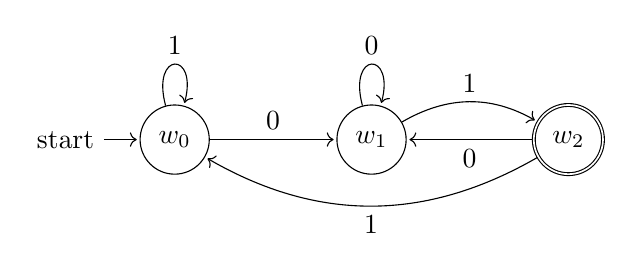
\begin{tikzpicture}[shorten >=1pt, node distance=2.5cm, on grid, auto] 
   \node[state, initial] (w0)   {$w_0$}; 
   \node[state, right of=w0] (w1) {$w_1$}; 
   \node[state, accepting, right of=w1] (w2) {$w_2$};

   \path[->] 
    (w0) edge [loop above] node {1} ()
         edge [left, above] node[above] {0} (w1)
    (w1) edge [loop above] node {0} ()
         edge [bend left, above] node {1} (w2)
    (w2) edge [bend left, below] node {1} (w0)
         edge [left, above] node[below] {0} (w1);
\end{tikzpicture}
}
\end{center}

In this DFA: 

\begin{enumerate}
    \item States: $W = \{w_0, w_1, w_2\}$
    \item Input Alphabet: $\Sigma = \{0, 1\}$
    \item Transition Function $V$:
    
    \[
    \begin{aligned}
        V(w_0, 0) &= w_1 \qquad & V(w_1, 1) &= w_2 \\
        V(w_0, 1) &= w_0 \qquad & V(w_2, 0) &= w_1 \\
        V(w_1, 0) &= w_1 \qquad & V(w_2, 1) &= w_0
    \end{aligned}
    \]

    \item Start State: $S = w_0$
    \item Accept State: $F = w_2$
\end{enumerate}

\subsection{Transition Table}

From that Transition Diagram we can construct a Transition Table as follow

\begin{center}
\begin{tabular}{c|cc} 
\textbf{W} & \textbf{0} & \textbf{1} \\ 
\hline $w_0$ & $w_1$ & $w_0$ 
\\ $w_1$ & $w_1$ & $w_2$ \\ 
$w_2$ & $w_1$ & $w_0$ \\ 
\end{tabular}
\end{center}

\subsection{Extended Transition Function}

The extended transition function $\hat{V}: W \times \Sigma^* \to W$ is defined by
\begin{enumerate}
    \item $\hat{V}(w,\varepsilon)=w,$ $\forall w\in W$.
    \item $\hat{V}(w,xy)=V\big(\hat{V}(w,x),y\big),$  $\forall w\in W$, $x\in\Sigma^*$, $y\in\Sigma$.
\end{enumerate}

Hence, from the above DFA we compute (starting from the start state $w_0$):

\begin{enumerate}[label={--}]
    \item $\hat{V}(w_0,\varepsilon) = w_0$
    \item $\hat{V}(w_0,0) = V(\hat{V}(w_0,\varepsilon),0) = w_1$
    \item $\hat{V}(w_0,1) = V(\hat{V}(w_0,\varepsilon),1) = w_0$
    \item $\hat{V}(w_0,01) = V(\hat{V}(w_0,0),1)  = w_2$
    \item $\hat{V}(w_0,101) = V(\hat{V}(w_0,10),1) = w_2$.
    \item $\hat{V}(w_0,1101) = V(\hat{V}(w_0,110),1) = w_2$.
    \item $\hat{V}(w_0,100) = V(\hat{V}(w_0,10),0) = w_1$.
\end{enumerate}

In general:

\[
\hat{V}(w_0, x) = F \;\Longleftrightarrow\; x \text{ ends with } xy,
\ \text{so} \
L(M) = \{\,x \in \{0,1\}^* \mid \hat{V}(w_0,x) \in F\,\}.
\]

\textbf{Example 1:}

Let

\[L(M_1) = \{0(0+1)^*\}\]

Hence

\begin{center}
\fbox{
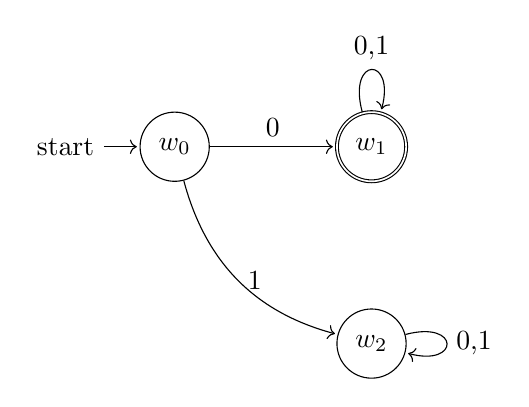
\begin{tikzpicture}[shorten >=1pt, node distance=2.5cm, on grid, auto] 
   
   \node[state, initial] (w0) {$w_0$}; 
   \node[state, accepting, right of=w0] (w1) {$w_1$}; 
   \node[state, below of=w1] (w2) {$w_2$};

   
   \path[->] 
      (w0) edge[above] node {0} (w1)
      (w0) edge[bend right] node[right] {1} (w2)
      (w1) edge[loop above] node {0,1} ()
      (w2) edge[loop right] node {0,1} ();
\end{tikzpicture}
}
\end{center}


Specifically, it only accept the input strings that start with 0. Oterwise, it goes to the dead state $w_2$. Formally,

\[
L(M_1)=
\begin{cases}
\{\,0x \mid x \in \{0,1\}^*\,\}, & \text{if the first symbol is } 0,\\[6pt]
\varnothing, & \text{otherwise}.
\end{cases}
\]


\newpage
\begin{enumerate}
    \item Transition Function $V$:
    
    \[
    \begin{aligned}
        V(w_0, 0) &= w_1 \qquad & V(w_1, 1) &= w_1 \\
        V(w_0, 1) &= w_2 \qquad & V(w_2, 0) &= w_2 \\
        V(w_1, 0) &= w_1 \qquad & V(w_2, 1) &= w_2
    \end{aligned}
    \]

    \item Transition Table:

    \begin{center}
    \begin{tabular}{c|cc}
    \textbf{W} & \textbf{0} & \textbf{1} \\
    \hline
    $w_0$ & $w_1$ & $w_2$ \\
    $w_1$ & $w_1$ & $w_1$ \\
    $w_2$ & $w_2$ & $w_2$ \\
    \end{tabular}
    \end{center}

\end{enumerate}



\section {Two-way Finite Automata (2DFA)}

Formally, $V: W \times (\Sigma \cup \{\triangleright,\#\}) \to W \times \{L, R\}$ is the \text{transition function}, where $\#$ is the end-of-tape marker and $\triangleright$ is the start-of-tape marker.

\begin{center}
\fbox{
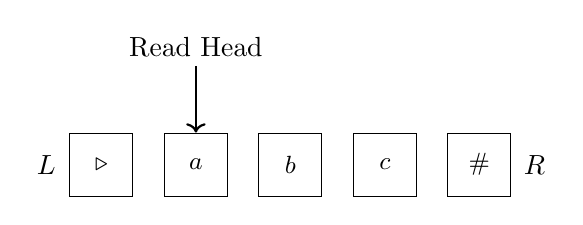
\begin{tikzpicture}[node distance=1.2cm]
    
    \node[draw, minimum size=0.8cm] (tape0) {\small $\triangleright$};
    \node[draw, minimum size=0.8cm, right of=tape0] (tape1) {\small $a$};
    \node[draw, minimum size=0.8cm, right of=tape1] (tape2) {\small $b$};
    \node[draw, minimum size=0.8cm, right of=tape2] (tape3) {\small $c$};
    \node[draw, minimum size=0.8cm, right of=tape3] (tape4) {\small $\#$};
    
    
    \node[above of=tape1, node distance=1.5cm] (head) {Read Head};
    \draw[->, thick] (head) -- (tape1);
    
    
    \node[left of=tape0, node distance=0.7cm] (left) {$L$};
    \node[right of=tape4, node distance=0.7cm] (right) {$R$};
\end{tikzpicture}
}
\end{center}

\textbf{In general:}

\[V(w_i, a) = (w_j, R)\]
This means that when the 2DFA is in state $w_i$ and reads the symbol $a$, it transitions to state $w_j$ and moves the read head one cell to the right (R).

\begin{center}
\fbox{
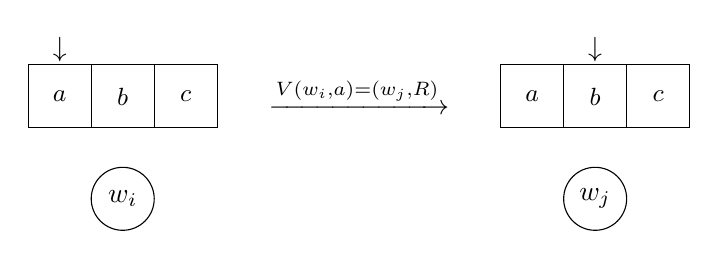
\begin{tikzpicture}[node distance=1.5cm]
    
    \node[draw, minimum size=0.8cm] (tape_b0) {\small $a$};
    \node[draw, minimum size=0.8cm, right of=tape_b0, node distance=0.8cm] (tape_b1) {\small $b$};
    \node[draw, minimum size=0.8cm, right of=tape_b1, node distance=0.8cm] (tape_b2) {\small $c$};
    
    \node[above of=tape_b0, node distance=0.6cm] (head_b) {$\downarrow$};
    
    \node[draw, circle, minimum size=0.8cm, below of=tape_b1, node distance=1.3cm] (state_b) {$w_i$};
    
    
    \node[right of=tape_b2, node distance=2.2cm] (arrow) {$\xrightarrow{V(w_i, a) = (w_j, R)}$};
    
    
    \node[draw, minimum size=0.8cm, right of=arrow, node distance=2.2cm] (tape_a0) {\small $a$};
    \node[draw, minimum size=0.8cm, right of=tape_a0, node distance=0.8cm] (tape_a1) {\small $b$};
    \node[draw, minimum size=0.8cm, right of=tape_a1, node distance=0.8cm] (tape_a2) {\small $c$};
    
    \node[above of=tape_a1, node distance=0.6cm] (head_a) {$\downarrow$};
    
    \node[draw, circle, minimum size=0.8cm, below of=tape_a1, node distance=1.3cm] (state_a) {$w_j$};
\end{tikzpicture}
}
\end{center}


Intuitively, a 2DFA operates like a standard DFA 

\begin{center}
\fbox{
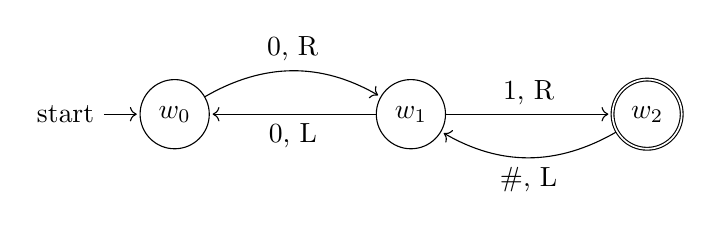
\begin{tikzpicture}[shorten >=1pt,node distance=3cm,on grid,auto]
    \node[state, initial] (w0) {$w_0$};
    \node[state] (w1) [right=of w0] {$w_1$};
    \node[state, accepting] (w2) [right=of w1] {$w_2$};

    \path[->]
    (w0) edge[bend left] node {0, R} (w1)
    (w1) edge[above] node {1, R} (w2)
    (w2) edge[bend left] node {\#, L} (w1)
    (w1) edge[below] node {0, L} (w0);
\end{tikzpicture}
}
\end{center}


\textbf{Example:} 

Let

\begin{center}
\fbox{
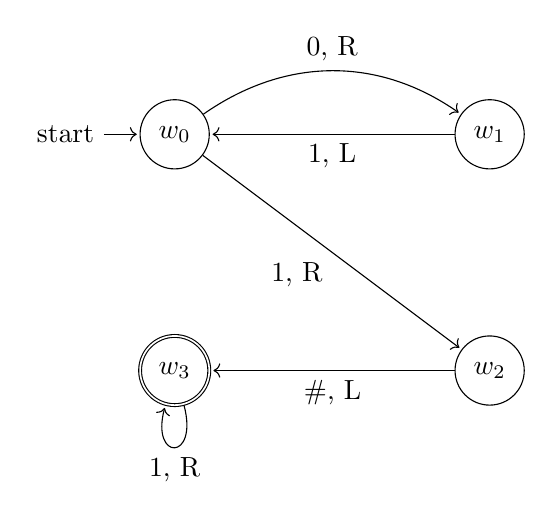
\begin{tikzpicture}[shorten >=1pt, on grid, auto]
    \node[state, initial] (w0) {$w_0$};
    \node[state] (w1) [right=4cm of w0] {$w_1$};
    \node[state] (w2) [below=3cm of w1] {$w_2$};
    \node[state, accepting] (w3) [left=4cm of w2] {$w_3$};

    \path[->]
    (w0) edge[bend left=35, above] node {0, R} (w1)
    (w1) edge[left=20, below] node {1, L} (w0)
    (w0) edge[below left] node {1, R} (w2)
    (w2) edge[below] node {\#, L} (w3)
    (w3) edge[loop below] node {1, R} ();
\end{tikzpicture}
}
\end{center}

This 2DFA accepts only the string $1$. The transition function is defined as:

\[
\begin{aligned}
    V(w_0, 0) &= (w_1, R) \qquad & V(w_2, \#) &= (w_3, L) \\
    V(w_0, 1) &= (w_2, R) \qquad & V(w_3, 1) &= (w_3, R) \\
    V(w_1, 1) &= (w_0, L)      &
\end{aligned}
\]

\begin{enumerate}

\item \textbf{Accepted:} Input $1$
\begin{enumerate}[label={--}]
\item Start: $w_0$, $\boxed{\underline{\mathtt{1}}}\boxed{\#}\boxed{\sqcup}\boxed{\sqcup}\boxed{\sqcup}\cdots$
\item Read $\mathtt{1}$, move R: $w_2$, $\boxed{\mathtt{1}}\boxed{\underline{\#}}\boxed{\sqcup}\boxed{\sqcup}\boxed{\sqcup}\cdots$
\item Read $\#$, move L: $w_3$, $\boxed{\underline{\mathtt{1}}}\boxed{\#}\boxed{\sqcup}\boxed{\sqcup}\boxed{\sqcup}\cdots$
\item Read $\mathtt{1}$, move R: $w_3$, $\boxed{\mathtt{1}}\boxed{\underline{\#}}\boxed{\sqcup}\boxed{\sqcup}\boxed{\sqcup}\cdots$
\item Accept (in state $w_3$ at end marker)
\end{enumerate}

\item \textbf{Rejected (crash):} Input $0$
\begin{enumerate}[label={--}]
\item Start: $w_0$, $\boxed{\underline{\mathtt{0}}}\boxed{\#}\boxed{\sqcup}\boxed{\sqcup}\boxed{\sqcup}\cdots$
\item Read $\mathtt{0}$, move R: $w_1$, $\boxed{\mathtt{0}}\boxed{\underline{\mathtt{1}}}\boxed{\#}\boxed{\sqcup}\boxed{\sqcup}\cdots$
\item Read $\mathtt{1}$: No transition for $(w_1, 1)$, Crash
\end{enumerate}

\item \textbf{Rejected (crash):} Input $11$
\begin{enumerate}[label={--}]
\item Start: $w_0$, $\boxed{\underline{\mathtt{1}}}\boxed{\mathtt{1}}\boxed{\#}\boxed{\sqcup}\boxed{\sqcup}\cdots$
\item Read $\mathtt{1}$, move R: $w_2$, $\boxed{\mathtt{1}}\boxed{\underline{\mathtt{1}}}\boxed{\#}\boxed{\sqcup}\boxed{\sqcup}\cdots$
\item Read $\mathtt{1}$: No transition for $(w_2, 1)$, Crash
\end{enumerate}

\item \textbf{Rejected (crash):} Input $10$
\begin{enumerate}[label={--}]
\item Start: $w_0$, $\boxed{\underline{\mathtt{1}}}\boxed{\mathtt{0}}\boxed{\#}\boxed{\sqcup}\boxed{\sqcup}\cdots$
\item Read $\mathtt{1}$, move R: $w_2$, $\boxed{\mathtt{1}}\boxed{\underline{\mathtt{0}}}\boxed{\#}\boxed{\sqcup}\boxed{\sqcup}\cdots$
\item Read $\mathtt{0}$: No transition for $(w_2, 0)$, Crash
\end{enumerate}

\item \textbf{Infinite loop:} Input $01$
\begin{enumerate}[label={--}]
\item Start: $w_0$, $\boxed{\underline{\mathtt{0}}}\boxed{\mathtt{1}}\boxed{\#}\boxed{\sqcup}\boxed{\sqcup}\cdots$
\item Read $\mathtt{0}$, move R: $w_1$, $\boxed{\mathtt{0}}\boxed{\underline{\mathtt{1}}}\boxed{\#}\boxed{\sqcup}\boxed{\sqcup}\cdots$
\item Read $\mathtt{1}$, move L: $w_0$, $\boxed{\underline{\mathtt{0}}}\boxed{\mathtt{1}}\boxed{\#}\boxed{\sqcup}\boxed{\sqcup}\cdots$
\item Read $\mathtt{0}$, move R: $w_1$, $\boxed{\mathtt{0}}\boxed{\underline{\mathtt{1}}}\boxed{\#}\boxed{\sqcup}\boxed{\sqcup}\cdots$
\item Read $\mathtt{1}$, move L: $w_0$, $\boxed{\underline{\mathtt{0}}}\boxed{\mathtt{1}}\boxed{\#}\boxed{\sqcup}\boxed{\sqcup}\cdots$
\item Cycles indefinitely between steps 3–5, Infinite loop
\end{enumerate}

\item \textbf{Infinite loop:} Input $010101$
\begin{enumerate}[label={--}]
\item Start: $w_0$, $\boxed{\underline{\mathtt{0}}}\boxed{\mathtt{1}}\boxed{\mathtt{0}}\boxed{\mathtt{1}}\boxed{\mathtt{0}}\boxed{\mathtt{1}}\boxed{\#}\cdots$
\item Read $\mathtt{0}$, move R: $w_1$, $\boxed{\mathtt{0}}\boxed{\underline{\mathtt{1}}}\boxed{\mathtt{0}}\boxed{\mathtt{1}}\boxed{\mathtt{0}}\boxed{\mathtt{1}}\boxed{\#}\cdots$
\item Read $\mathtt{1}$, move L: $w_0$, $\boxed{\underline{\mathtt{0}}}\boxed{\mathtt{1}}\boxed{\mathtt{0}}\boxed{\mathtt{1}}\boxed{\mathtt{0}}\boxed{\mathtt{1}}\boxed{\#}\cdots$
\item Cycles between positions 0 and 1, Infinite loop
\end{enumerate}

\end{enumerate}

\section{Non-deterministic Finite Automata (NFA)}

An NFA is similar like DFA, but a state can have zero, one, or many possible transitions for the same input symbol, and it may even move without consuming input ($\varepsilon$-Transition). 
It’s more flexible in structure, though it recognizes the same class of languages as a DFA. 
Formally, an NFA is defined as a 5-tuple $M = (W, \Sigma, V, S, F)$ where $V: W \times \Sigma \to 2^{|W|}$, and the language it recognizes is defined as: $L(M)= \{x \mid V(w, x) \cap F \neq \varnothing\}.$


\textbf{Example:} 

Let 

\[
L(M) = \{\, x \in \{0,1\}^* \mid x \text{ contains the substring } 010 \,\}
\]

\begin{center}
\fbox{
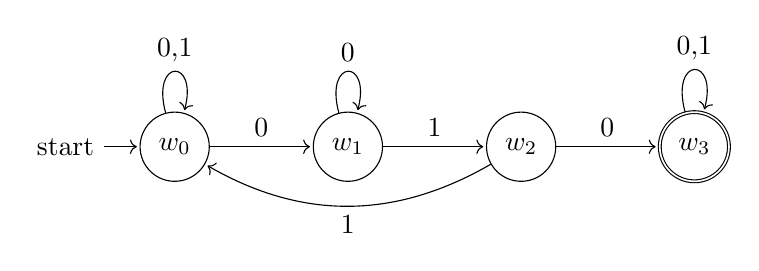
\begin{tikzpicture}[shorten >=1pt, node distance=2.2cm, on grid, auto]

  \node[state, initial] (w0) {$w_0$};
  \node[state] (w1) [right of=w0] {$w_1$};
  \node[state] (w2) [right of=w1] {$w_2$};
  \node[state, accepting] (w3) [right of=w2] {$w_3$};

  \path[->]
    (w0) edge[loop above] node {0,1} ()
    (w0) edge[left] node[above] {0} (w1)

    (w1) edge node {1} (w2)
    (w1) edge[loop above] node {0} ()

    (w2) edge node {0} (w3)
    (w2) edge[bend left] node[below] {1} (w0)

    (w3) edge[loop above] node {0,1} ();
\end{tikzpicture}
}
\end {center}

\newpage
In this NFA: 

\begin{enumerate}
    \item Transition Function $V$:
    
    \[
    \begin{aligned}
        V(w_0, 0) &= \{w_0, w_1\} \qquad & V(w_2, 0) &= \{w_3\} \\
        V(w_0, 1) &= \{w_0\}        \qquad & V(w_2, 1) &= \{w_0\} \\
        V(w_1, 0) &= \{w_1\}        \qquad & V(w_3, 0) &= \{w_3\} \\
        V(w_1, 1) &= \{w_2\}        \qquad & V(w_3, 1) &= \{w_3\}
    \end{aligned}
    \]



    \item Transition Table: 
    
    \begin{center}
    \begin{tabular}{c|cc}
    \textbf{W} & \textbf{0} & \textbf{1} \\
    \hline
    $w_0$ & $\{w_0, w_1\}$ & $\{w_0\}$ \\
    $w_1$ & $\{w_1\}$ & $\{w_2\}$ \\
    $w_2$ & $\{w_3\}$ & $\{w_0\}$ \\
    $w_3$ & $\{w_3\}$ & $\{w_3\}$ \\
    \end{tabular}
    \end{center}

\end{enumerate}

\subsection{$\varepsilon$-NFA}

An $\varepsilon$-NFA is an extension of the NFA that allows transitions without consuming any input symbols, known as $\varepsilon$-transitions.

\textbf{Example:}

Let 

\[
L(M) = \{\, x \in \{0,1\}^* \mid x \text{ can reach } w_2 \text{ using } \varepsilon\text{-transitions or by reading a } 1 \,\}
\]

\begin{center}
\fbox{
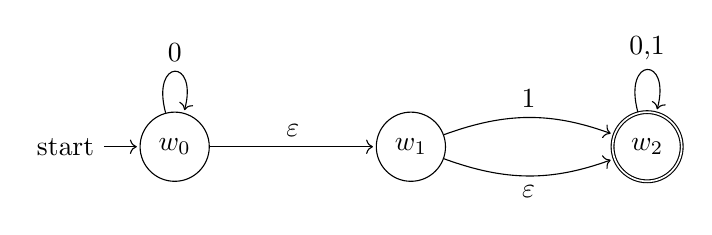
\begin{tikzpicture}[shorten >=1pt, node distance=3cm, on grid, auto]

  \node[state, initial] (w0) {$w_0$};
  \node[state] (w1) [right of=w0] {$w_1$};
  \node[state, accepting] (w2) [right of=w1] {$w_2$};

  
  \path[->]
    (w0) edge[loop above] node {0} ()
    (w0) edge node[above] {$\varepsilon$} (w1)

    (w1) edge[bend left=20] node[above] {1} (w2)
    (w1) edge[bend right=20] node[below] {$\varepsilon$} (w2)

    (w2) edge[loop above] node {0,1} ();

\end{tikzpicture}
}
\end{center}


In this $\varepsilon$-NFA:

\begin{enumerate}

    \item Transition Function $V$:
    
    
    \[
    \begin{aligned}
        V(w_0, \varepsilon) &= \{w_1\} \qquad & V(w_1, \varepsilon) &= \{w_2\} \\
        V(w_0, 0)           &= \{w_0\} \qquad & V(w_2, 0)           &= \{w_2\} \\
        V(w_1, 1)           &= \{w_2\} \qquad & V(w_2, 1)           &= \{w_2\}
    \end{aligned}
    \]


    \item Transition Table:

    \begin{center}
    \begin{tabular}{c|ccc}
    \textbf{W} & \textbf{0} & \textbf{1} & $\boldsymbol{\varepsilon}$\\
    \hline
    $w_0$ & $\{w_0\}$ & $\varnothing$ & $\{w_1\}$ \\
    $w_1$ & $\varnothing$ & $\{w_2\}$ & $\{w_2\}$ \\
    $w_2$ & $\{w_2\}$ & $\{w_2\}$ & $\varnothing$ \\
    \end{tabular}
    \end{center}

\end{enumerate}

\subsection{$\varepsilon$-Closure}

The $\varepsilon$-closure of a state $w$ is the set of all states reachable 
from $w$ using only $\varepsilon$-transitions, including $w$ itself. For the $\varepsilon$-NFA above:

\begin{enumerate}
    \item $\varepsilon(w_0) = \{ w_0, w_1, w_2 \}$ \ 
    (since $w_0 \xrightarrow{\varepsilon} w_1 \xrightarrow{\varepsilon} w_2$)

    \item $\varepsilon(w_1) = \{ w_1, w_2 \}$ \ 
    (since $w_1 \xrightarrow{\varepsilon} w_2$)

    \item $\varepsilon(w_2) = \{ w_2 \}$ \
    (no $\varepsilon$-transitions from $w_2$)
\end{enumerate}

Thus, the $\varepsilon$-closures can be summarized in the following table:

\begin{center}
\begin{tabular}{c|c}
\textbf{W} & \textbf{$\varepsilon$-Closure} \\
\hline
$w_0$ & $\{w_0, w_1, w_2\}$ \\
$w_1$ & $\{w_1, w_2\}$ \\
$w_2$ & $\{w_2\}$ \\
\end{tabular}
\end{center}

Moreover, the extended Transition Function for $\varepsilon$-NFA is defined as:

\begin{enumerate}[label={--}]
    \item $\hat{V}(w_0,\varepsilon)
      = \varepsilon(w_0)
      = \{w_0, w_1, w_2\}$

    \item $\hat{V}(w_0,0)
      = V(\varepsilon(w_0),0)
      = V(\{w_0,w_1,w_2\},0)
      = \{w_0,w_2\}$

    \item $\hat{V}(w_0,1)
      = V(\varepsilon(w_0),1)
      = V(\{w_0,w_1,w_2\},1)
      = \{w_2\}$
\end{enumerate}

\section{Conversion}

\subsection{NFA to DFA }

\begin{enumerate}
    \item Given an NFA  
    \[
    N = (W, \Sigma, V, S, F)
    \]
    \item the equivalent DFA  
    \[
    D = (W', \Sigma, V', S', F')
    \]
\end{enumerate}

where 

\[
\begin{aligned}
W' &= 2^{|W|} & V'(X, a) &= \varepsilon\text{-closure}\left(\bigcup_{w \in X} V(w, a)\right) \\
S' &= \varepsilon\text{-closure}(S) & F' &= \{\, X \in W' \mid X \cap F \neq \varnothing \,\}
\end{aligned}
\]

\newpage

\textbf{In general}

\begin{enumerate}
    
\item NFA

\begin{center}
\fbox{
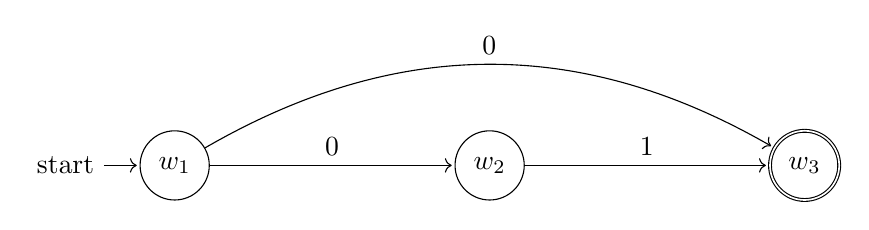
\begin{tikzpicture}[shorten >=1pt,node distance=4cm,on grid,auto]
   \node[state, initial] (w1) {$w_1$};
   \node[state] (w2) [right=of w1] {$w_2$};
   \node[state, accepting] (w3) [right=of w2] {$w_3$};

   \path[->]
   (w1) edge node {0} (w2)
   (w1) edge [bend left] node {0} (w3)
   (w2) edge node {1} (w3);
\end{tikzpicture}
}
\end{center}

\item Transition Table

\begin{center}
\begin{tabular}{c|cc}
\textbf{W} & \textbf{0} & \textbf{1} \\
\hline
$w_1$ & $\{w_2, w_3\}$ & $w_1$ \\
$w_2$ & $\varnothing$ & $w_3$ \\
$w_3$ & $\varnothing$ & $\varnothing$ \\
\end{tabular}
\end{center}

\item DFA 

\begin{center}
\fbox{
\begin{tikzpicture}[shorten >=1pt, node distance=4cm, on grid, auto]


\node[state, initial] (w1) {$w_1$};
\node[state, accepting] (w23) [right=of w1] {$w_2,w_3$};
\node[state, accepting] (w3) [right=of w23] {$w_3$};
\node[state] (empty) [right=of w3] {$\varnothing$};


\path[->]
(w1) edge node[above] {0} (w23)
(w1) edge[bend left=45] node[above] {1} (empty);


\path[->]
(w23) edge node[above] {1} (w3)
(w23) edge[bend right=25] node[below] {0} (empty);


\path[->]
(w3) edge[loop above] node {0,1} (w3);


\path[->]
(empty) edge[loop above] node {0,1} (empty);

\end{tikzpicture}
}
\end{center}

\item DFA Transition Table

\begin{center}
\begin{tabular}{c|cc}
\textbf{W} & \textbf{0} & \textbf{1} \\
\hline
$w_1$ & $\{w_2,w_3\}$ & $\varnothing$ \\
$\{w_2,w_3\}$ & $\varnothing$ & $\{w_3\}$ \\
$w_3$ & $w_3$ & $w_3$ \\
$\varnothing$ & $\varnothing$ & $\varnothing$ \\
\end{tabular}
\end{center}


\end{enumerate}


\begin{enumerate}

\item \textbf{Example 1:}

Consider the NFA, where

\[
W = \{w_1, w_2, w_3\}, \quad 
\Sigma = \{0,1\}, \quad
F = \{w_3\},
\]

and the transition function \(V\) is defined as:

\[
\begin{aligned}
V(w_1,0) &= \{w_2\},      &\qquad V(w_2,0) &= \{w_2\}, \\
V(w_1,1) &= \{w_2,w_3\}, &\qquad V(w_3,0) &= \{w_3\}, \\
V(w_2,1) &= \{w_3\},     &\qquad V(w_3,1) &= \{w_3\}. \\
\end{aligned}
\]

\begin{enumerate}

\item NFA

\begin{center}
\fbox{
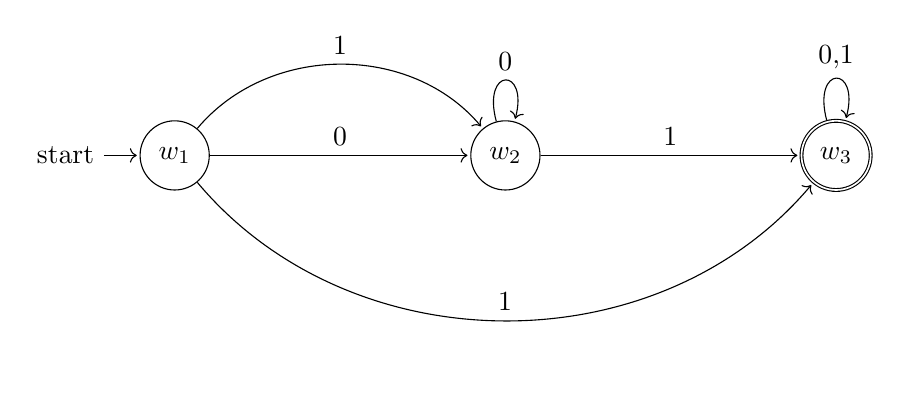
\begin{tikzpicture}[shorten >=1pt,node distance=4.2cm,on grid,auto]
   \node[state, initial] (w1) {$w_1$};
   \node[state] (w2) [right=of w1] {$w_2$};
   \node[state, accepting] (w3) [right=of w2] {$w_3$};

   \path[->]
   (w1) edge node {0} (w2)
   (w1) edge [bend left=50] node {1} (w2)
   (w1) edge [bend right=50] node {1} (w3)
   (w2) edge node {1} (w3)
   (w2) edge[loop above] node {0} (w2)
   (w3) edge[loop above] node {0,1} (w3);
\end{tikzpicture}
}
\end{center}

\item Transition Table

\begin{center}
\begin{tabular}{c|cc}
\textbf{W} & \textbf{0} & \textbf{1} \\
\hline
$w_1$ & $w_2$ & $\{w_2, w_3\}$ \\
$w_2$ & $w_2$ & $w_3$ \\
$w_3$ & $w_3$ & $w_3$ \\
\end{tabular}
\end{center}

\item DFA Construction

\[
W' = 2^{|W|}, \quad S' = \{w_1\}, \quad F' = \{\, X \subseteq W \mid X \cap \{w_3\} \neq \varnothing \,\}
\]

\noindent

\begin{center}
\fbox{
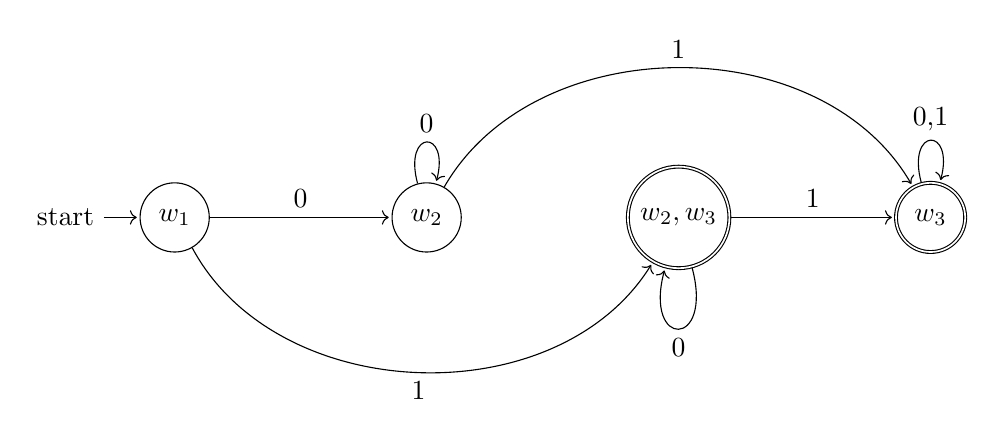
\begin{tikzpicture}[shorten >=1pt,node distance=3.2cm,on grid,auto]
    \node[state, initial] (w1) {$w_1$};
    \node[state] (w2) [right=of w1] {$w_2$};
    \node[state, accepting] (w23) [right=of w2] {$w_2,w_3$};
    \node[state, accepting] (w3) [right=of w23] {$w_3$};

    \path[->]
        (w1) edge node {0} (w2)
        (w1) edge[bend right=60] node[below] {1} (w23)
        (w2) edge[loop above] node {0} (w2)
        (w2) edge[bend left=60] node[above] {1} (w3)
        (w23) edge[loop below] node {0} (w23)
        (w23) edge node {1} (w3)
        (w3) edge[loop above] node {0,1} (w3);
\end{tikzpicture}
}
\end{center}

\item DFA Transition Table

\[
\begin{array}{c|c|c}
\textbf{W} & \textbf{0} & \textbf{1} \\ \hline
w_1     & w_2       & \{w_2,w_3\} \\
w_2     & w_2       & w_3     \\
w_3     & w_3       & w_3     \\
\{w_2,w_3\} & \{w_2,w_3\}   & w_3     \\
\end{array}
\]

\end{enumerate}

\item \textbf{Example 2:}

Consider the NFA:

\[
W = \{w_1,w_2,w_3\}, 
\qquad 
\Sigma = \{0,1\}, 
\qquad
F = \{w_3\},
\]

with transition function

\[
\begin{aligned}
V(w_1,0) &= \{w_1,w_2\}, &\qquad V(w_2,0) &= \{w_1\}, &\qquad V(w_3,0) &= \varnothing, \\[4pt]
V(w_1,1) &= \{w_3\},     &\qquad V(w_2,1) &= \{w_2\}, &\qquad V(w_3,1) &= \{w_1,w_2\}.
\end{aligned}
\]

\end{enumerate}

\begin{enumerate}

\item NFA

\begin{center}
\fbox{
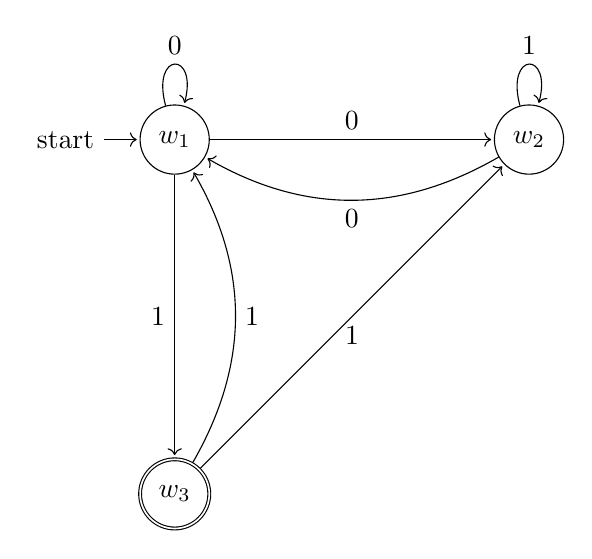
\begin{tikzpicture}[shorten >=1pt,node distance=4.5cm,on grid,auto]
   \node[state, initial] (w1) {$w_1$};
   \node[state] (w2) [right=of w1] {$w_2$};
   \node[state, accepting] (w3) [below=of w1] {$w_3$};

   \path[->]
   (w1) edge[loop above] node {$0$} (w1)
   (w1) edge node[above] {$0$} (w2)
   (w1) edge node[left] {$1$} (w3)

   (w2) edge[loop above] node {$1$} (w2)
   (w2) edge[bend left=30] node[below] {$0$} (w1)

   (w3) edge[bend right=30] node[right] {$1$} (w1)
   (w3) edge node[below] {$1$} (w2);
\end{tikzpicture}
}
\end{center}

\item DFA Transition Table

\[
\begin{array}{c|c|c}
\textbf{W} & \textbf{0} & \textbf{1} \\ \hline
w_1       & \{w_1,w_2\} & w_3       \\ 
\{w_1,w_2\}   & \{w_1,w_2\} & \{w_2,w_3\}   \\
w_3       & \varnothing & \{w_1,w_2\}   \\
\{w_2,w_3\}   & w_1     & \{w_1,w_2\}   \\
\end{array}
\]


\end{enumerate}


\subsection{NFA to $\varepsilon$-NFA}

Consider the NFA:
\[
W=\{w_1,w_2,w_3\},\quad F=\{w_3\}
\]

\begin{center}
\begin{tabular}{c|cc}
\textbf{W} & \textbf{0} & \textbf{1} \\
\hline
$w_1$ & $\{w_1,w_2\}$ & $\{w_2\}$ \\
$w_2$ & $\{w_3\}$ & $\{w_1\}$ \\
$w_3$ & $\varnothing$ & $\{w_3\}$ \\
\end{tabular}
\end{center}

Since an NFA is automatically an $\varepsilon$-NFA, then we can define the equivalent $\varepsilon$-NFA as:

\begin{center}
\begin{tabular}{c|ccc}
\textbf{W} & \textbf{$\varepsilon$} & \textbf{0} & \textbf{1} \\
\hline
$w_1$ & $\{w_2\}$ & $\{w_1,w_2\}$ & $\{w_2\}$ \\
$w_2$ & $\{w_3\}$ & $\{w_3\}$ & $\{w_1\}$ \\
$w_3$ & $\varnothing$ & $\varnothing$ & $\{w_3\}$ \\
\end{tabular}
\end{center}


\subsection{$\varepsilon$-NFA to NFA}

Let 

\[
W = \{w_1,w_2,w_3,w_4,w_5,w_6\}, \quad \Sigma = \{0,1\}, \quad F = \{w_4\}
\]

\begin{center}
\begin{tabular}{c|ccc}
\textbf{W} & \textbf{0} & \textbf{1} & \textbf{$\varepsilon$} \\
\hline
$w_1$ & $\{w_5\}$ & $\{w_2\}$ & $\varnothing$ \\
$w_2$ & $\varnothing$ & $\{w_3\}$ & $\{w_4\}$ \\ 
$w_3$ & $\varnothing$ & $\{w_4\}$ & $\varnothing$ \\
$w_4$ & $\varnothing$ & $\varnothing$ & $\varnothing$ \\
$w_5$ & $\{w_6\}$ & $\varnothing$ & $\{w_2,w_3\}$ \\
$w_6$ & $\{w_4\}$ & $\varnothing$ & $\varnothing$ \\
\end{tabular}
\end{center}

\[
\begin{aligned}
    \varepsilon(w_1) &= \{w_1\}, \qquad & \varepsilon(w_4) &= \{w_4\} \\
    \varepsilon(w_2) &= \{w_2,w_4\}, \qquad & \varepsilon(w_5) &= \{w_5,w_2,w_3,w_4\} \\
    \varepsilon(w_3) &= \{w_3\}, \qquad & \varepsilon(w_6) &= \{w_6\}
\end{aligned}
\]

\begin{center}
\begin{tabular}{c|cc}
\textbf{W} & \textbf{0} & \textbf{1} \\
\hline
$w_1$ & $\{w_5\}$ & $\{w_2\}$ \\
$w_2$ & $\varnothing$ & $\{w_3\}$ \\ 
$w_3$ & $\varnothing$ & $\{w_4\}$ \\
$w_4$ & $\varnothing$ & $\varnothing$ \\
$w_5$ & $\{w_6\}$ & $\{w_3,w_4\}$ \\
$w_6$ & $\{w_4\}$ & $\varnothing$ \\
\end{tabular}
\end{center}

The accept states of the NFA are

\[
F_N = \{w_2,w_4,w_5\}.
\]

\subsection{Finite Automata (FA) to Regular Expressions (RE)}

Given a DFA $M=(W,\Sigma,V,S,F)$, define the regular expression $R_{ij}^{(k)}$ as the set of all strings that take the DFA from state $w_i$ to state $w_j$ without passing through any intermediate states with an index greater than $k$.
\[
R_{ij}^{(k)} = R_{ij}^{(k-1)} + R_{ik}^{(k-1)} (R_{kk}^{(k-1)})^* R_{kj}^{(k-1)},
\qquad
R = \bigcup_{w_f\in F} R_{S,w_f}^{(|W|)}.
\]

\subsection*{Example}

Consider the DFA:
\[
W=\{w_0,w_1,w_2\},\quad
\Sigma=\{a,b\},\quad
S=w_0,\quad
F=\{w_2\}.
\]

Transition function:
\[
\begin{aligned}
V(w_0,a)=w_1,\; \qquad& V(w_0,b)=w_0,\\
V(w_1,a)=w_1,\;\qquad& V(w_1,b)=w_2,\\
V(w_2,a)=w_2,\;\qquad& V(w_2,b)=w_2.
\end{aligned}
\]

Base step

\[
\begin{array}{c|ccc}
& w_0 & w_1 & w_2 \\ \hline
w_0 & \varepsilon+b & a & \varnothing \\[2pt]
w_1 & \varnothing & \varepsilon+a & b \\[2pt]
w_2 & \varnothing & \varnothing & \varepsilon+a+b
\end{array}
\]


\begin{center}
\fbox{
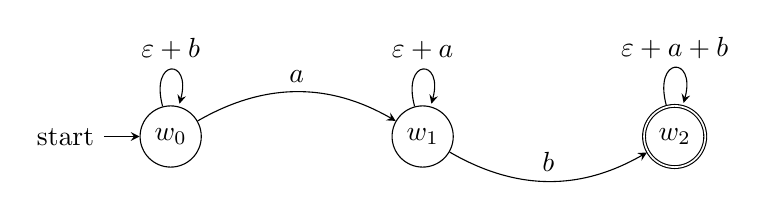
\begin{tikzpicture}[->,>=stealth,node distance=32mm]
\tikzstyle{every state}=[minimum size=18pt]

\node[state, initial] (w0) {$w_0$};
\node[state] (w1) [right of=w0] {$w_1$};
\node[state, accepting] (w2) [right of=w1] {$w_2$};

\path
(w0) edge[loop above] node{$\varepsilon+b$} ()
edge[bend left] node[above]{$a$} (w1)
(w1) edge[loop above] node{$\varepsilon+a$} ()
edge[bend right] node[above]{$b$} (w2)
(w2) edge[loop above] node{$\varepsilon+a+b$} ();
\end{tikzpicture}
}
\end{center}


\newpage

Eliminate $w_1$

\begin{align*}
   &\quad \underbrace{\text{from } w_i \text{ to } w_1}_{R_{i1}}
                             \;\;\underbrace{\text{loop inside } w_1}_{(R_{11})^*} 
                             \;\;\underbrace{\text{from } w_1 \text{ to } w_j}_{R_{1j}} \\[1mm]
\end{align*}

Combine both cases:

\[R'_{ij} = R_{ij} + R_{i1} (R_{11})^* R_{1j}\]

\begin{align*}
R'_{ij} &= R_{ij} + \underbrace{R_{i1}(R_{11})^*R_{1j}}_{\ } \\[2mm]
R'_{0,2} &= R_{0,2} + a(\varepsilon+a)^* b 
         = \varnothing + a(\varepsilon+a)^* b 
         = a a^* b \\[2mm]
R'_{0,0} &= R_{0,0} + a(\varepsilon+a)^* \varnothing
         = (\varepsilon + b) + a(\varepsilon+a)^*\varnothing
         = \varepsilon + b \\[2mm]
R'_{2,2} &= R_{2,2} + \varnothing(\varepsilon+a)^* b
         = (\varepsilon + a + b) + \varnothing(\varepsilon+a)^* b
         = \varepsilon + a + b
\end{align*}



\begin{center}
\fbox{
\begin{tikzpicture}[->,>=stealth,node distance=48mm]
  \tikzstyle{every state}=[minimum size=18pt]

  \node[state, initial] {$w_0$};
  \node[state, accepting] (w2) [right of=w0] {$w_2$};

  \path
    (w0) edge[loop above] node{$\varepsilon+b$} ()
    (w2) edge[loop above] node{$\varepsilon+a+b$} ()
    (w0) edge[bend left] node[above]{$a\,a^*\,b$} (w2);
\end{tikzpicture}
}
\end{center}

Hence

\[
R = (R'_{0,0})^*\, R'_{0,2}\, (R'_{2,2})^*
= (\varepsilon+b)^*\,(a a^* b)\,(\varepsilon+a+b)^*.
\]

\begin{center}
\fbox{
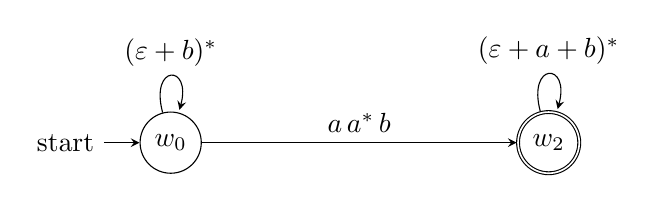
\begin{tikzpicture}[->,>=stealth,node distance=48mm]
  \tikzstyle{every state}=[minimum size=18pt]

  \node[state, initial] (w0) {$w_0$};
  \node[state, accepting] (w2) [right of=w0] {$w_2$};

  \path
    (w0) edge[loop above] node{$(\varepsilon+b)^*$} ()
    (w2) edge[loop above] node{$(\varepsilon+a+b)^*$} ()
    (w0) edge node[above]{$a\,a^*\,b$} (w2);
\end{tikzpicture}
}
\end{center}

\begin{align*}
R &= (\varepsilon+b)^* (a a^* b) (\varepsilon + a + b)^* \\[2mm]
  &= (b^*\, a a^* b\, (a+b)^*) \\[1mm]
  &= ((a+b)^* a b (a+b)^*) \\[1mm]
  &= (a \mid b)^* a b (a \mid b)^*
\end{align*}

Compactly as:

\[
\boxed{R = (a\mid b)^*\, a\, b\, (a\mid b)^* }.
\]

\section{Moore and Mealy Machine}

\subsection{Moore Machine}

Formally, a Moore machine is defined as a 6-tuple

\[M = (W, \Sigma, \Delta, V, \lambda, S)\]

where

\begin{enumerate}
    \item $\Delta$ is the output alphabet,
    \item $\lambda: W \to \Delta$ is the output function that maps each state to an output symbol.
\end{enumerate}

\textbf{Example:}

Let $W = \{w_0, w_1, w_2, w_3, w_4, w_5, w_6\}$, $\Sigma = \{0, 1\}$, $\Delta = \{g, e, n, s, i\}$, and $S = w_0$.

\begin{enumerate}
    \item Transition Function $V$ and Output Function $\lambda$:

        \begin{center}
            \begin{tabular}{c|cc}
            \textbf{W} & \textbf{0} & \textbf{1} \\
            \hline
            $w_0$ & $w_1$ & $w_0$ \\
            $w_1$ & $w_2$ & $w_1$ \\
            $w_2$ & $w_3$ & $w_2$ \\
            $w_3$ & $w_4$ & $w_3$ \\
            $w_4$ & $w_5$ & $w_4$ \\
            $w_5$ & $w_6$ & $w_5$ \\
            $w_6$ & $w_6$ & $w_6$ \\
            \end{tabular}
            \end{center}

\begin{center}
\fbox{
\begin{tikzpicture}[shorten >=1pt, node distance=4cm, on grid, auto]

    
    \node[state, initial] (w0) at (90:3.5) {$w_0 / g$};     
    \node[state]          (w1) at (30:3.5) {$w_1 / e$};     
    \node[state]          (w2) at (-30:3.5) {$w_2 / n$};    
    \node[state]          (w3) at (-90:3.5) {$w_3 / e$};    
    \node[state]          (w4) at (-150:3.5) {$w_4 / s$};   
    \node[state]          (w5) at (150:3.5) {$w_5 / i$};    

    
    \node[state] (w6) at (0,0) {$w_6 / s$};

   
    \path[->]
        (w0) edge node {0} (w1)
        (w1) edge node {0} (w2)
        (w2) edge node {0} (w3)
        (w3) edge node {0} (w4)
        (w4) edge node {0} (w5)
        (w5) edge node {0} (w6);

    
    \path[->]
        (w0) edge[loop above] node {1} ()
        (w1) edge[loop above] node {1} ()
        (w2) edge[loop right] node {1} ()
        (w3) edge[loop below] node {1} ()
        (w4) edge[loop left] node {1} ()
        (w5) edge[loop left] node {1} ();

   
    \path[->]
        (w6) edge[loop above] node {0,1} ();

\end{tikzpicture}
}
\end{center}


Operation on input string $000000$:

        \begin{center}
        \begin{tabular}{c|c|c}
        \textbf{Input} & \textbf{State} & \textbf{Output} \\
        \hline
        -- & $w_0$ & $g$ \\
        $0$ & $w_1$ & $e$ \\
        $0$ & $w_2$ & $n$ \\
        $0$ & $w_3$ & $e$ \\
        $0$ & $w_4$ & $s$ \\
        $0$ & $w_5$ & $i$ \\
        $0$ & $w_6$ & $s$ \\
        \end{tabular}
        \end{center}

        Hence, final output sequence: $\boxed{genesis}$

\end{enumerate}

\subsection{Mealy Machine}

Bassically, a Mealy machine is defined as a 6-tuple, just like the Moore machine:   
\[M = (W, \Sigma, \Delta, V, \lambda, S)\]

In this case, if Moore machine's output function maps states to outputs, Mealy machine's output function maps state-input pairs to outputs:
\begin{enumerate}
    \item $\Delta$ is the output alphabet,
    \item $\lambda: W \times \Sigma \to \Delta$ is the output function that maps each state-input pair to an output symbol,
    \item The output is determined by the transition: $\lambda(w, x) = y$, where $w \in W$, $x \in \Sigma$, and $y \in \Delta$.
\end{enumerate}

\textbf{Example:}

Let $W = \{w_0, w_1, w_2, w_3, w_4, w_5\}$, $\Sigma = \{0, 1\}$, $\Delta = \{e, x, o, d, u, s\}$, and $S = w_0$.

\begin{enumerate}
    \item Transition Function $V$ and Output Function $\lambda$:

        
        
            \[
            \begin{aligned}
            V(w_0, 0) = w_1, \qquad & \lambda(w_0, 0) = e, \\
            V(w_1, 0) = w_2, \qquad & \lambda(w_1, 0) = x, \\
            V(w_2, 0) = w_3, \qquad & \lambda(w_2, 0) = o, \\
            V(w_3, 0) = w_4, \qquad & \lambda(w_3, 0) = d, \\
            V(w_4, 0) = w_5, \qquad & \lambda(w_4, 0) = u, \\
            V(w_5, 0) = w_5, \qquad & \lambda(w_5, 0) = s.
            \end{aligned}
            \]

        
          
        \begin{center}
        \fbox{
        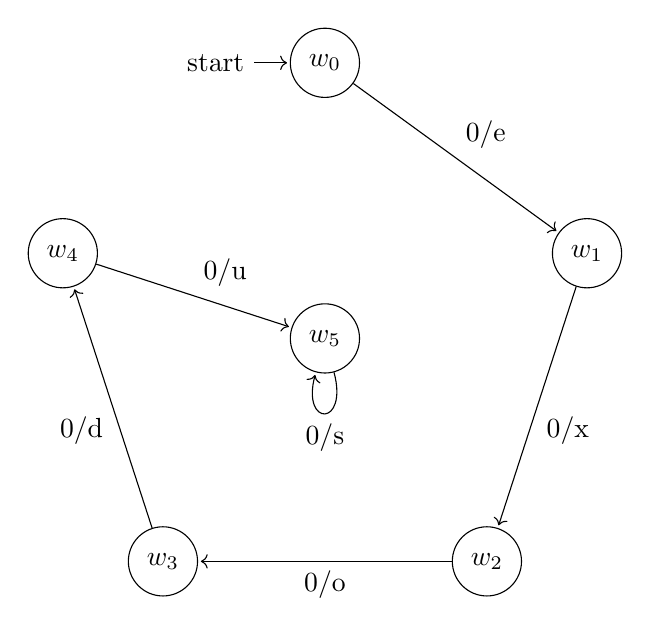
\begin{tikzpicture}[shorten >=1pt, node distance=4cm, on grid, auto]

            
            \node[state, initial] (w0) at (90:3.5) {$w_0$};
            \node[state]          (w1) at (18:3.5) {$w_1$};
            \node[state]          (w2) at (-54:3.5) {$w_2$};
            \node[state]          (w3) at (-126:3.5) {$w_3$};
            \node[state]          (w4) at (-198:3.5) {$w_4$};

            \node[state] (w5) at (0, 0) {$w_5$};

            \path[->]
                (w0) edge node {0/e} (w1)
                (w1) edge node {0/x} (w2)
                (w2) edge node {0/o} (w3)
                (w3) edge node {0/d} (w4)
                (w4) edge node {0/u} (w5)
                (w5) edge[loop below] node {0/s} ();

        \end{tikzpicture}
        }
        \end{center}


Operation on input string $000000$:

        \begin{center}
        \begin{tabular}{c|c|c|c}
        \textbf{Input} & \textbf{State} & \textbf{Output} & \textbf{Transition} \\
        \hline
        -- & $w_0$ & -- & -- \\
        $0$ & $w_1$ & $e$ & $V(w_0, 0) = w_1, \lambda(w_0, 0) = e$ \\
        $0$ & $w_2$ & $x$ & $V(w_1, 0) = w_2, \lambda(w_1, 0) = x$ \\
        $0$ & $w_3$ & $o$ & $V(w_2, 0) = w_3, \lambda(w_2, 0) = o$ \\
        $0$ & $w_4$ & $d$ & $V(w_3, 0) = w_4, \lambda(w_3, 0) = d$ \\
        $0$ & $w_5$ & $u$ & $V(w_4, 0) = w_5, \lambda(w_4, 0) = u$ \\
        $0$ & $w_5$ & $s$ & $V(w_5, 0) = w_5, \lambda(w_5, 0) = s$ \\
        \end{tabular}
        \end{center}

    Hence, final output sequence: $\boxed{exodus}$

\end{enumerate}

\newpage

\subsection{Moore to Mealy}

To convert a Moore machine to an equivalent Mealy machine, we adjust the
output function so that outputs are associated with transitions rather
than states.

Given a Moore machine defined as:

\[
M_{o} = (W, \Sigma, \Delta, V, \lambda, S),
\]

we construct an equivalent Mealy machine:

\[
M_{e} = (W, \Sigma, \Delta, V, \lambda', S),
\]

where the new output function $\lambda'$ is defined by:

\[
\lambda'(w, x) = \lambda(V(w, x))
\quad\forall\, w \in W,\ \forall\, x \in \Sigma.
\]

This ensures that the Mealy machine produces, during each transition,
the same output that the Moore machine produces upon entering the next state.


\textbf{Example:}

Let $W = \{w_0, w_1, w_2, w_3, w_4, w_5\}$, $\Sigma = \{0, 1\}$, $\Delta = \{u, t, o, p, i, a\}$, and $S = w_0$.

\begin{enumerate}
    \item \textbf{Moore Machine}
    
    Transition Function $V$ and Output Function $\lambda$:
    
    \begin{center}
    \begin{tabular}{c|cc|c}
    \textbf{W} & \textbf{0} & \textbf{1} & \textbf{Output} \\
    \hline
    $w_0$ & $w_1$ & $w_0$ & $u$ \\
    $w_1$ & $w_2$ & $w_1$ & $t$ \\
    $w_2$ & $w_3$ & $w_2$ & $o$ \\
    $w_3$ & $w_4$ & $w_3$ & $p$ \\
    $w_4$ & $w_5$ & $w_4$ & $i$ \\
    $w_5$ & $w_5$ & $w_5$ & $a$ \\
    \end{tabular}
    \end{center}
    
\begin{center}
\fbox{
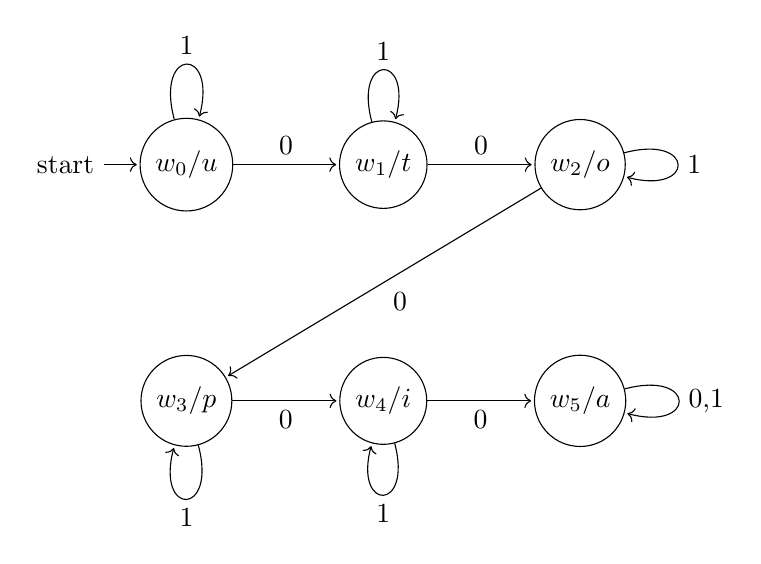
\begin{tikzpicture}[shorten >=1pt, node distance=2cm, on grid, auto]

    \node[state, initial] (w0) at (0, 3) {$w_0/u$};
    \node[state]          (w1) at (2.5, 3) {$w_1/t$};
    \node[state]          (w2) at (5, 3) {$w_2/o$};
    \node[state]          (w3) at (0, 0) {$w_3/p$};
    \node[state]          (w4) at (2.5, 0) {$w_4/i$};
    \node[state]          (w5) at (5, 0) {$w_5/a$};

    \path[->]
        (w0) edge node {0} (w1)
        (w0) edge[loop above] node {1} ()
        
        (w1) edge node {0} (w2)
        (w1) edge[loop above] node {1} ()
        
        (w2) edge node {0} (w3)
        (w2) edge[loop right] node {1} ()
        
        (w3) edge node[below] {0} (w4)
        (w3) edge[loop below] node {1} ()
        
        (w4) edge node[below] {0} (w5)
        (w4) edge[loop below] node {1} ()
        
        (w5) edge[loop right] node {0,1} ();

\end{tikzpicture}
}
\end{center}


    \item \textbf{Mealy Machine}
    
    Using $\lambda'(w, x) = \lambda(V(w, x))$, we compute:
    
    \begin{center}
    \begin{tabular}{c|cc}
    \textbf{W} & \textbf{0} & \textbf{1} \\
    \hline
    $w_0$ & $w_1/t$ & $w_0/u$ \\
    $w_1$ & $w_2/o$ & $w_1/t$ \\
    $w_2$ & $w_3/p$ & $w_2/o$ \\
    $w_3$ & $w_4/i$ & $w_3/p$ \\
    $w_4$ & $w_5/a$ & $w_4/i$ \\
    $w_5$ & $w_5/a$ & $w_5/a$ \\
    \end{tabular}
    \end{center}
        
\begin{center}
\fbox{
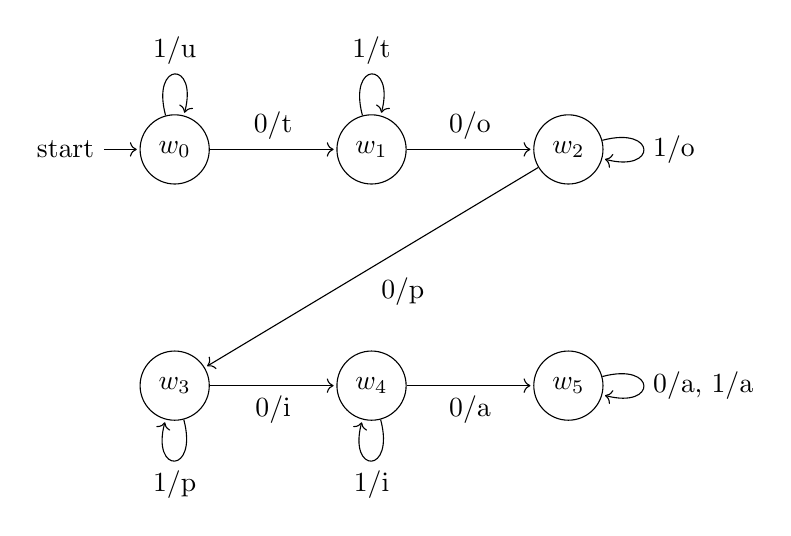
\begin{tikzpicture}[shorten >=1pt, node distance=2cm, on grid, auto]

    \node[state, initial] (w0) at (0, 3) {$w_0$};
    \node[state]          (w1) at (2.5, 3) {$w_1$};
    \node[state]          (w2) at (5, 3) {$w_2$};
    \node[state]          (w3) at (0, 0) {$w_3$};
    \node[state]          (w4) at (2.5, 0) {$w_4$};
    \node[state]          (w5) at (5, 0) {$w_5$};

    \path[->]
        (w0) edge node {0/t} (w1)
        (w0) edge[loop above] node {1/u} ()
        
        (w1) edge node {0/o} (w2)
        (w1) edge[loop above] node {1/t} ()
        
        (w2) edge node {0/p} (w3)
        (w2) edge[loop right] node {1/o} ()
        
        (w3) edge node[below] {0/i} (w4)
        (w3) edge[loop below] node {1/p} ()
        
        (w4) edge node[below] {0/a} (w5)
        (w4) edge[loop below] node {1/i} ()
        
        (w5) edge[loop right] node {0/a, 1/a} ();

\end{tikzpicture}
}
\end{center}

    
    \item \textbf{Comparison on input string } $00000$:
    
    \begin{center}
    \begin{tabular}{c|c|c|c}
    \textbf{Input} & \textbf{State} & \textbf{Moore Output} &  \textbf{Mealy Output} \\
    \hline
    -- & $w_0$ & $u$ &  -- \\
    $0$ & $w_1$ & $t$ &  $t$ \\
    $0$ & $w_2$ & $o$ &  $o$ \\
    $0$ & $w_3$ & $p$ &  $p$ \\
    $0$ & $w_4$ & $i$ & $i$ \\
    $0$ & $w_5$ & $a$ &  $a$ \\
    \end{tabular}
    \end{center}

    Hence, both machines produce the same output sequence: $\boxed{utopia}$

\end{enumerate}

\subsection{Mealy to Moore}


To convert a Mealy machine to an equivalent Moore machine, we must modify the
state space so that outputs are associated with states rather than transitions.

Let the Mealy machine be defined as
\[
M_{e} = (W, \Sigma, \Delta, V, \lambda, S),
\]
where \( \lambda : W \times \Sigma \to \Delta \).

We construct an equivalent Moore machine
\[
M_{o} = (W', \Sigma, \Delta, V', \lambda', S')
\]
as follows.

\begin{enumerate}
    \item State set

    \[
    W' = \{\, (w, y) \mid w \in W,\ y \in \Delta,\ \exists x \in \Sigma \text{ such that } \lambda(w,x) = y \,\}
    \]

    Each state \((w,y)\) represents being in Mealy state \(w\) with output \(y\).

    \item Initial state

    Since a Mealy machine produces output only after reading an input symbol,
    we introduce a new symbol \(s_\bot \notin W'\) to serve as the initial state.
    \[
    S' = s_\bot
    \]

    \item Output function

    \[
    \lambda'(s_\bot) = \varepsilon
    \]
    \[
    \lambda'((w,y)) = y \quad \forall (w,y) \in W'
    \]

    \item Transition function

    From the initial symbol:
    \[
    V'(s_\bot, x) = (V(S,x), \lambda(S,x)) \quad \forall x \in \Sigma
    \]

    For all other states:
    \[
    V'((w,y), x) = (V(w,x), \lambda(w,x)) \quad \forall (w,y) \in W',\ \forall x \in \Sigma
    \]
\end{enumerate}

The resulting Moore machine is equivalent to the original Mealy machine with
respect to input/output behavior. The construction may introduce unreachable
states; therefore, only states reachable from \(S'\) need to be retained to
obtain a minimal equivalent Moore machine.

\textbf{Example:}

\begin{enumerate}

\item \textbf{Mealy Machine}

\[
W = \{w_0, w_1, w_2\}, \quad 
\Sigma = \{0, 1\}, \quad 
\Delta = \{x,y\}, \quad 
S = w_0
\]

With this transition

\begin{center}
\begin{tabular}{c|cc}
W & 0 & 1 \\
\hline
$w_0$ & $w_1/x$ & $w_2/x$ \\
$w_1$ & $w_1/y$ & $w_2/x$ \\
$w_2$ & $w_1/x$ & $w_2/y$ \\
\end{tabular}
\end{center}

\begin{center}
\fbox{
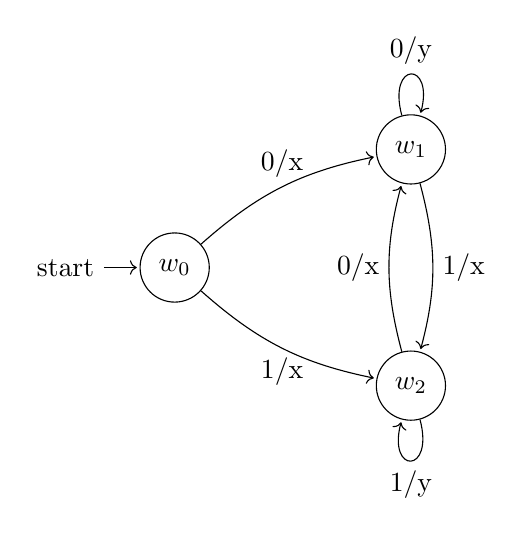
\begin{tikzpicture}[shorten >=1pt, node distance=3cm, on grid, auto]

    
    \node[state, initial] (w0) at (0,0) {$w_0$};
    \node[state] (w1) at (3,1.5) {$w_1$};
    \node[state] (w2) at (3,-1.5) {$w_2$};

    
    \path[->]
        
        (w0) edge[bend left=15] node[above] {0/x} (w1)
        (w0) edge[bend right=15] node[below] {1/x} (w2)

        
        (w1) edge[loop above] node {0/y} ()
        (w1) edge[bend left=15] node {1/x} (w2)

        
        (w2) edge[bend left=15] node {0/x} (w1)
        (w2) edge[loop below] node {1/y} ();

\end{tikzpicture}
}
\end{center}

\item \textbf{Moore Machine}

All reachable states:

\[
W' = \{ s_\bot \cup (w_1,x), (w_1,y), (w_2,x), (w_2,y) \} 
\]

With this transition

\begin{center}
\begin{tabular}{c|cc}
$W'$ &   0 & 1 \\
\hline
$s_\bot$ &  $w_1,x$ & $w_2,x$ \\
$w_1,x$ & $w_1,y$ & $w_2,x$ \\
$w_1,y$ &  $w_1,y$ & $w_2,x$ \\
$w_2,x$ &  $w_1,x$ & $w_2,y$ \\
$w_2,y$ &  $w_1,x$ & $w_2,y$ \\
\end{tabular}
\end{center}


\begin{center}
\fbox{
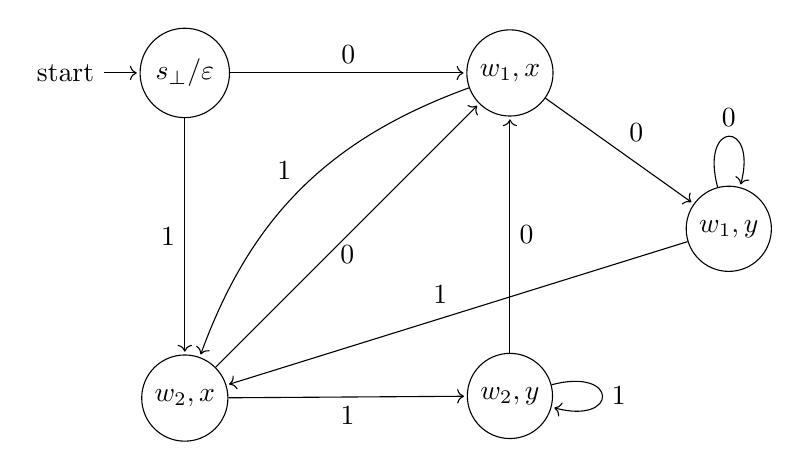
\begin{tikzpicture}[shorten >=1pt, node distance=3cm]
    
    \node[state, initial] (sb) {$s_\bot/\varepsilon$};
    \node[state] (w1x) [right=of sb] {$w_1,x$};
    \node[state] (w1y) [below right=1.2cm and 2cm of w1x] {$w_1,y$};
    \node[state] (w2x) [below=of sb] {$w_2,x$};
    \node[state] (w2y) [below=of w1x] {$w_2,y$};

    \path[->]
        (sb) edge node[above] {0} (w1x)
        (sb) edge node[left] {1} (w2x)
        
        (w1x) edge node[above right] {0} (w1y)
        (w1x) edge [bend right=25] node[above left] {1} (w2x)

        (w1y) edge[loop above] node {0} (w1y)
        (w1y) edge[left=160] node[above left] {1} (w2x)

        (w2x) edge node[below] {0} (w1x)
        (w2x) edge node[below] {1} (w2y)

        (w2y) edge[right=15] node[right] {0} (w1x)
        (w2y) edge[loop right] node {1} (w2y);
\end{tikzpicture}
}
\end{center}

\end{enumerate}



\section{Property of Regular Languages}
 
\subsection{Decision Algorithms}

A language is regular if there exists a finite automaton that recognizes it. The following decision problems can be solved for regular languages:

\subsubsection{Emptiness}

\[L(M) = \varnothing \leftrightarrow \forall f \in F, \ f \text{ is not reachable from } S\]

A DFA $M$ has an \textbf{empty language} if no accepting state can be reached from the initial state.

\textbf{Example:} 

Let $M = (W,\Sigma,V,S,F)$ where

\[
W = \{q_0,q_1,q_2\},\quad
\Sigma = \{0,1\},\quad
S = q_0,\quad
F = \{q_2\}.
\]

\begin{center}
\fbox{
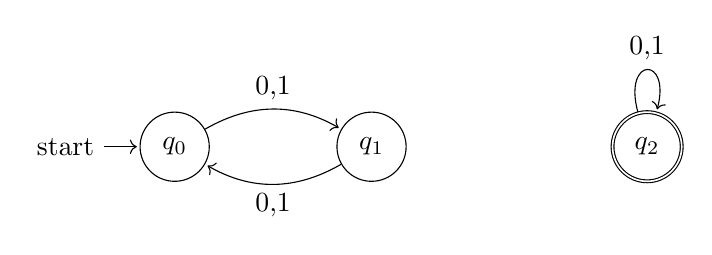
\begin{tikzpicture}[shorten >=1pt, node distance=2.5cm, on grid, auto]

    \node[state, initial] (q0) at (0, 0) {$q_0$};
    \node[state]          (q1) at (2.5, 0) {$q_1$};
    \node[state, accepting] (q2) at (6, 0) {$q_2$};

    \path[->]
        (q0) edge[bend left] node {0,1} (q1)
        (q1) edge[bend left] node {0,1} (q0)
        (q2) edge[loop above] node {0,1} ();
\end{tikzpicture}
}
\end{center}

The accepting state $q_2$ is isolated and unreachable from the initial state $q_0$. Since there is no path from $q_0$ to $q_2$, no string can be accepted. Hence:
\[
L(M) = \varnothing.
\]


\subsubsection{Finiteness}

A language $L(M)$ is \textbf{finite} if it contains a finite number of strings, and \textbf{infinite} otherwise.

\begin{enumerate}

\item \textbf{Finite Language} 

\[L(M) \text{ is finite} \leftrightarrow \nexists w' \in W : S \xrightarrow{*} w' \xrightarrow{+} w' \xrightarrow{*} f, \ f \in F\]

A language is finite if there is no cycle on any path from the initial state to an accepting state.

\textbf{Example:}

DFA $M_1$ accepts $L = \{a, ab, abb\}$. Since $|L| = 3 < \infty$, the language is finite. 

Let $M_1 = (W, \Sigma, V, S, F)$ where:

\[
W = \{q_0, q_1, q_2, q_3, q_4\},\quad
\Sigma = \{a,b\},\quad
S = q_0,\quad
F = \{q_1, q_2, q_3\}.
\]

\begin{center}
\fbox{
\begin{tikzpicture}[shorten >=1pt, node distance=3cm, on grid, auto]

    \node[state, initial] (q0) at (0, 0) {$q_0$};
    \node[state, accepting] (q1) at (3, 0) {$q_1$};
    \node[state, accepting] (q2) at (6, 0) {$q_2$};
    \node[state, accepting] (q3) at (9, 0) {$q_3$};
    \node[state] (q4) at (6, -2.5) {$q_4$};

    \path[->]
        (q0) edge node[above] {$a$} (q1)
        (q1) edge node[above] {$b$} (q2)
        (q2) edge node[above] {$b$} (q3)
        (q3) edge[left=20] node[right] {$a,b$} (q4)
        (q4) edge[loop below] node {$a,b$} ()
        (q0) edge[loop above] node {$b$} ()
        (q1) edge[left=30] node[left] {$a$} (q4);
\end{tikzpicture}
}
\end{center}

The language is finite because there are no cycles on any path from $S$ to accepting states $\{q_1, q_2, q_3\}$.

\item \textbf{Infinite Language}

\[L(M) \text{ is infinite} \leftrightarrow \exists w' \in W : S \xrightarrow{*} w' \xrightarrow{+} w' \xrightarrow{*} f, \ f \in F\]

A language is infinite if there exists a cycle on some path from the initial state to an accepting state.

\textbf{Example:}

DFA $M_2$ accepts $L = \{a^n \mid n \geq 1\}$, which is infinite. 

Let $M_2 = (W, \Sigma, V, S, F)$ where:

\[
W = \{q_0, q_1\},\quad
\Sigma = \{a,b\},\quad
S = q_0,\quad
F = \{q_1\}.
\]

\begin{center}
\fbox{
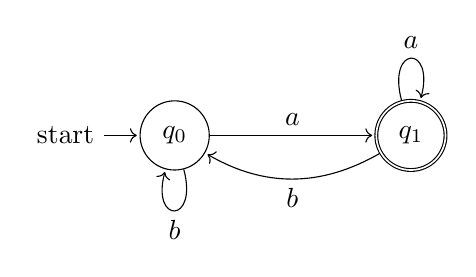
\begin{tikzpicture}[shorten >=1pt, node distance=3cm, on grid, auto]

    \node[state, initial] (q0) at (0, 0) {$q_0$};
    \node[state, accepting] (q1) at (3, 0) {$q_1$};

    \path[->]
        (q0) edge node[above] {$a$} (q1)
        (q1) edge[loop above] node {$a$} ()
        (q0) edge[loop below] node {$b$} ()
        (q1) edge[bend left] node[below] {$b$} (q0);
\end{tikzpicture}
}
\end{center}

The language is infinite because state $q_1$ has a self-loop (cycle), is reachable from $S$, and is an accepting state, satisfying $S \xrightarrow{*} q_1 \xrightarrow{+} q_1$.

\end{enumerate}

\subsubsection{Membership}


\[x \in L(M) \leftrightarrow V^*(S, x) \in F\]

where $V^*$ is the extended transition function that processes the entire string $x$ from the start state $S$.

\textbf{Example:} 
    
Given DFA $M = (W, \Sigma, V, S, F)$ with $L(M) = \{w \in \{0,1\}^* \mid w \text{ ends in } 01\}$ where:

\[
W = \{q_0, q_1, q_2\},\quad
\Sigma = \{0,1\},\quad
S = q_0,\quad
F = \{q_2\}.
\]

Transition table:

\begin{center}
\begin{tabular}{c|cc}
$V$ & $0$ & $1$ \\
\hline
$q_0$ & $q_1$ & $q_0$ \\
$q_1$ & $q_1$ & $q_2$ \\
$q_2$ & $q_1$ & $q_0$ \\
\end{tabular}
\end{center}

\begin{center}
\fbox{
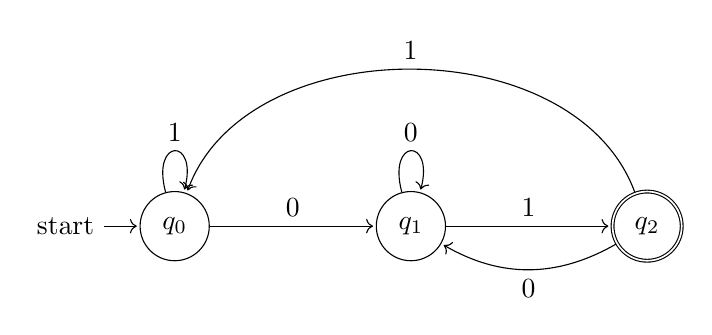
\begin{tikzpicture}[shorten >=1pt, node distance=2.5cm, on grid, auto]

    \node[state, initial] (q0) at (0, 0) {$q_0$};
    \node[state] (q1) at (3, 0) {$q_1$};
    \node[state, accepting] (q2) at (6, 0) {$q_2$};

    \path[->]
        (q0) edge[loop above] node {$1$} (q0)
        (q0) edge node {$0$} (q1)
        (q1) edge[loop above] node {$0$} (q1)
        (q1) edge node {$1$} (q2)
        (q2) edge[bend left] node[below] {$0$} (q1)
        (q2) edge[bend right=70] node[above] {$1$} (q0);
\end{tikzpicture}
}
\end{center}

Testing membership: Does $x = 1001 \in L(M)$?

We trace the computation step by step:

\begin{align*}
V(q_0, 1) &= q_0 \\
V(q_0, 0) &= q_1 \\
V(q_1, 0) &= q_1 \\
V(q_1, 1) &= q_2
\end{align*}

Since $V^*(q_0, 1001) = q_2 \in F$, the string $x = 1001$ is accepted. Therefore, $ x \in L(M)$. 

The string $1001$ ends in $01$, confirming membership in the language.

\subsubsection{Equivalence}

\[M_1 \equiv M_2 \leftrightarrow L(M_1) = L(M_2)\]

Two DFAs $M_1$ and $M_2$ are equivalent if and only if they accept exactly the same language, i.e., for all strings $x \in \Sigma^*$:
\[x \in L(M_1) \leftrightarrow x \in L(M_2)\]

\textbf{Example:} 

Consider two DFAs that both accept strings with an even number of $0$'s over $\Sigma = \{0,1\}$.

\textbf{DFA $M_1$}:

$M_1 = (W_1, \Sigma, V_1, S_1, F_1)$ where:

\[
W_1 = \{q_0, q_1\},\quad
\Sigma = \{0,1\},\quad
S_1 = q_0,\quad
F_1 = \{q_0\}.
\]

\begin{center}
\begin{tabular}{c|cc}
State & $0$ & $1$ \\
\hline
$q_0$ & $q_1$ & $q_0$ \\
$q_1$ & $q_0$ & $q_1$ \\
\end{tabular}
\end{center}

\begin{center}
\fbox{
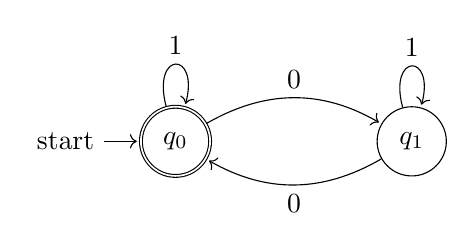
\begin{tikzpicture}[shorten >=1pt, node distance=3cm, on grid, auto]
    \node[state, initial, accepting] (q0) at (0, 0) {$q_0$};
    \node[state] (q1) at (3, 0) {$q_1$};

    \path[->]
        (q0) edge[loop above] node {$1$} (q0)
        (q0) edge[bend left] node[above] {$0$} (q1)
        (q1) edge[loop above] node {$1$} (q1)
        (q1) edge[bend left] node[below] {$0$} (q0);
\end{tikzpicture}
}
\end{center}

\textbf{DFA $M_2$}:

$M_2 = (W_2, \Sigma, V_2, S_2, F_2)$ where:

\[
W_2 = \{p_0, p_1, p_2, p_3\},\quad
\Sigma = \{0,1\},\quad
S_2 = p_0,\quad
F_2 = \{p_0, p_2\}.
\]

\begin{center}
\begin{tabular}{c|cc}
State & $0$ & $1$ \\
\hline
$p_0$ & $p_1$ & $p_2$ \\
$p_1$ & $p_0$ & $p_3$ \\
$p_2$ & $p_3$ & $p_0$ \\
$p_3$ & $p_2$ & $p_1$ \\
\end{tabular}
\end{center}

\begin{center}
\fbox{
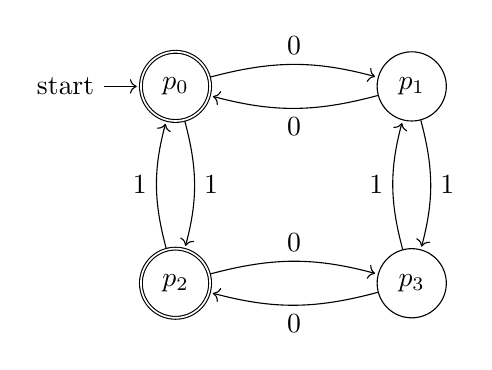
\begin{tikzpicture}[shorten >=1pt, node distance=3cm, on grid, auto]
    \node[state, initial, accepting] (p0) at (0, 0) {$p_0$};
    \node[state] (p1) at (3, 0) {$p_1$};
    \node[state, accepting] (p2) at (0, -2.5) {$p_2$};
    \node[state] (p3) at (3, -2.5) {$p_3$};

    \path[->]
        (p0) edge[bend left=15] node[above] {$0$} (p1)
        (p0) edge[bend left=15] node[right] {$1$} (p2)

        (p1) edge[bend left=15] node[below] {$0$} (p0)
        (p1) edge[bend left=15] node[right] {$1$} (p3)

        (p2) edge[bend left=15] node[above] {$0$} (p3)
        (p2) edge[bend left=15] node[left] {$1$} (p0)

        (p3) edge[bend left=15] node[below] {$0$} (p2)
        (p3) edge[bend left=15] node[left] {$1$} (p1);
\end{tikzpicture}
}
\end{center}

Let's test several strings to verify both DFAs accept the same language:

\begin{enumerate}
    \item $x = \varepsilon$: $M_1$ ends at $q_0$, $M_2$ ends at $p_0$  (0 zeros, even)
    \item $x = 00$: $M_1$ ends at $q_0$, $M_2$ ends at $p_0$  (2 zeros, even)
    \item $x = 101$: $M_1$ ends at $q_1$, $M_2$ ends at $p_3$  (1 zero, odd)
    \item $x = 0110$: $M_1$ ends at $q_0$, $M_2$ ends at $p_2$  (2 zeros, even)
\end{enumerate}

Both DFAs accept exactly the same language:

$$L(M_1) = L(M_2) = \{w \in \{0,1\}^* \mid \text{number of } 0\text{'s in } w \text{ is even}\}$$

Despite having different numbers of states and different structures, they recognize the same language. Therefore, $M_1 \equiv M_2$.

$M_2$ tracks both the parity of $0$'s (even/odd) and whether the last symbol was $0$ or $1$, making it non-minimal. States $p_0$ and $p_2$ are both accepting because they both represent an even number of $0$'s.

\subsubsection{Minimization}

A minimal DFA $M'$ for a language $L$ is a DFA such that
\[
L(M') = L \;\land\; \nexists \text{ DFA } M'' \text{ with } L(M'') = L \text{ and } |W''| < |W'|.
\]

For any DFA $M$ with $L(M) = L$, the minimization process produces such an automaton $M'$ by merging equivalent states, where $w \sim w'$ denotes that the states $w$ and $w'$ are equivalent.

\textbf{Example 1:}

Let $M = (W, \Sigma, V, S, F)$, where
\[
W = \{w_0,w_1,w_2,w_3,w_4\}, \quad \Sigma = \{0,1\}, \quad S = w_0, \quad F = \{w_4\}.
\]

The transition function is given by:

\[
\begin{tabular}{c|c|c}
$W$ & $0$ & $1$ \\
\hline
$w_0$ & $w_1$ & $w_2$ \\
$w_1$ & $w_1$ & $w_3$ \\
$w_2$ & $w_1$ & $w_2$ \\
$w_3$ & $w_1$ & $w_4$ \\
$w_4$ & $w_1$ & $w_2$
\end{tabular}
\]

\begin{center}
\fbox{
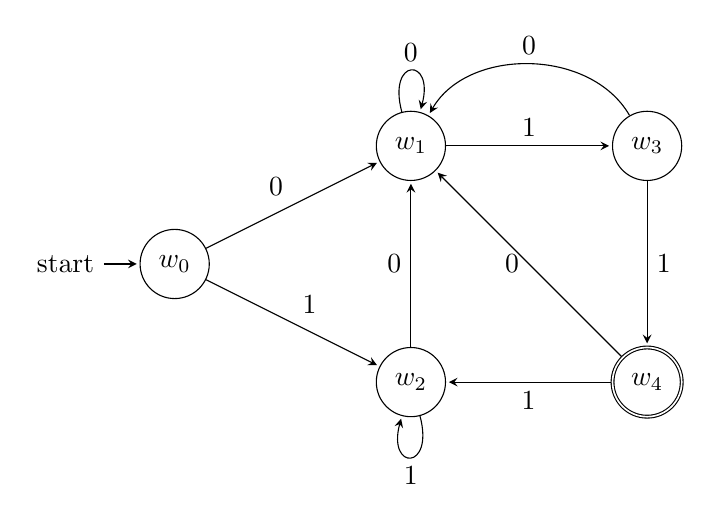
\begin{tikzpicture}[>=stealth,shorten >=1pt,auto]


\node[state, initial] (w0) at (0,0) {$w_0$};
\node[state] (w1) at (3,1.5) {$w_1$};
\node[state] (w2) at (3,-1.5) {$w_2$};
\node[state] (w3) at (6,1.5) {$w_3$};
\node[state, accepting] (w4) at (6,-1.5) {$w_4$};


\draw[->] (w0) -- node {0} (w1);
\draw[->] (w0) -- node {1} (w2);


\draw[->] (w1) edge[loop above] node {0} ();
\draw[->] (w1) -- node {1} (w3);


\draw[->] (w2) -- node[left] {0} (w1);
\draw[->] (w2) edge[loop below] node {1} ();


\draw[->, bend right=60] (w3) to node[above] {0} (w1);
\draw[->] (w3) -- node[right] {1} (w4);


\draw[->] (w4) -- node[left] {0} (w1);
\draw[->] (w4) -- node[below] {1} (w2);

\end{tikzpicture}
}
\end{center}

\begin{enumerate}
    \item For a DFA $M$, the $n$-equivalence relation $\equiv_n$ on states is defined inductively as follows:
    \[
    w \equiv_0 w' \;\Longleftrightarrow\; (w \in F \leftrightarrow w' \in F).
    \]
    \[
    w \equiv_{n+1} w' \;\Longleftrightarrow\;
    \bigl(w \equiv_0 w' \;\land\; \forall a \in \Sigma,\; V(w,a) \equiv_n V(w',a)\bigr).
    \]

    \item The equivalence relation used in DFA minimization is obtained when this sequence stabilizes:
    \[
    \exists k \in \mathbb{N} \text{ such that } \equiv_k = \equiv_{k+1}.
    \]

    \item The resulting equivalence relation can be characterized as:
    \[
    w \sim w' \;\Longleftrightarrow\;
    \forall x \in \Sigma^*,\;
    \bigl(V^*(w,x) \in F \leftrightarrow V^*(w',x) \in F\bigr).
    \]
\end{enumerate}

From the transition structure, we compute the successive partitions:

\begin{enumerate}
    \item \textbf{0-Equivalence:} Partition states by acceptance.
    \[
    \phi_0 = \bigl\{\{w_0,w_1,w_2,w_3\}, \{w_4\}\bigr\}
    \]

    \item \textbf{1-Equivalence:} Refine partitions based on transitions.

    For $\{w_0,w_1,w_2,w_3\}$:
    \begin{enumerate}
        \item $w_0$: $0 \to w_1$, $1 \to w_2$
        \item $w_1$: $0 \to w_1$, $1 \to w_3$
        \item $w_2$: $0 \to w_1$, $1 \to w_2$
        \item $w_3$: $0 \to w_1$, $1 \to w_4$
    \end{enumerate}

    Since $w_3$ transitions to an accepting state on input $1$, we split:
    \[
    \phi_1 = \bigl\{\{w_0,w_1,w_2\}, \{w_3\}, \{w_4\}\bigr\}
    \]

    \item \textbf{2-Equivalence:} Refine $\{w_0,w_1,w_2\}$.

    \begin{enumerate}
        \item $w_0$: $1 \to w_2 \in \{w_0,w_2\}$
        \item $w_1$: $1 \to w_3 \in \{w_3\}$
        \item $w_2$: $1 \to w_2 \in \{w_0,w_2\}$
    \end{enumerate}

    Thus,
    \[
    \phi_2 = \bigl\{\{w_0,w_2\}, \{w_1\}, \{w_3\}, \{w_4\}\bigr\}
    \]

    \item \textbf{3-Equivalence:} The block $\{w_0,w_2\}$ cannot be further refined, so
    \[
    \phi_3 = \phi_2.
    \]
\end{enumerate}

Hence, the minimal DFA merges $w_0$ and $w_2$ into a single state.  
The minimized DFA has states $\{\{w_0,w_2\}, w_1, w_3, w_4\}$.

\begin{center}
\fbox{
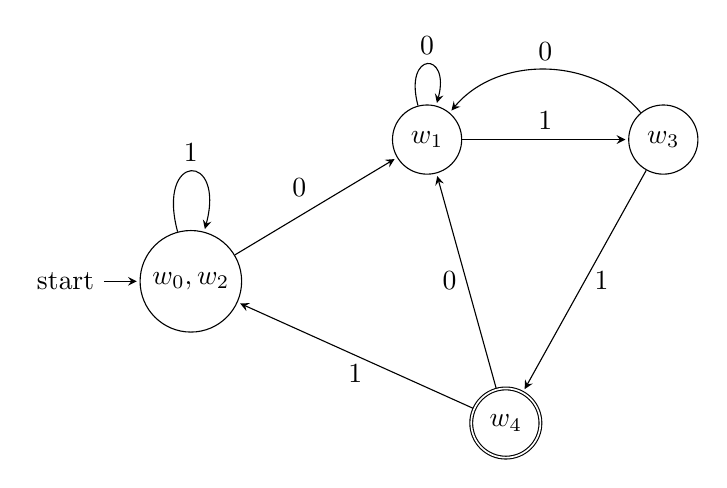
\begin{tikzpicture}[>=stealth,shorten >=1pt,auto]


\node[state, initial] (w02) at (0,0) {$w_0,w_2$};
\node[state] (w1) at (3,1.8) {$w_1$};
\node[state] (w3) at (6,1.8) {$w_3$};
\node[state, accepting] (w4) at (4,-1.8) {$w_4$};


\draw[->] (w02) -- node {0} (w1);
\draw[->] (w02) edge[loop above] node {1} ();

\draw[->] (w1) edge[loop above] node {0} ();
\draw[->] (w1) -- node {1} (w3);

\draw[->, bend right=50] (w3) to node[above] {0} (w1);
\draw[->] (w3) -- node[right] {1} (w4);

\draw[->] (w4) -- node[left] {0} (w1);
\draw[->] (w4) -- node[below] {1} (w02);

\end{tikzpicture}
}
\end{center}

\textbf{Example 2:}


Let

\[
M = (W, \Sigma, V, S, F)
\]

where

\[
W = \{w_0,w_1,w_2,w_3,w_4,w_5,w_6,w_7\}, \quad
\Sigma = \{0,1\}, \quad
S = w_0, \quad
F = \{w_2\}.
\]

The transition function is:

\[
\begin{array}{c|cc}
W & 0 & 1 \\ \hline
w_0 & w_1 & w_5 \\
w_1 & w_6 & w_2 \\
w_2 & w_0 & w_2 \\
w_3 & w_2 & w_6 \\
w_4 & w_7 & w_5 \\
w_5 & w_2 & w_6 \\
w_6 & w_6 & w_4 \\
w_7 & w_6 & w_2
\end{array}
\]


\begin{enumerate}



\item \textbf{0-Equivalence}

Partition states by acceptance:

\[
f_0 =
\bigl\{
\{w_2\},
\{w_0,w_1,w_3,w_4,w_5,w_6,w_7\}
\bigr\}
\]


\item \textbf{1-Equivalence}

Refine the non-accepting block by transitions:

\[
\begin{array}{c|cc}
W & 0 & 1 \\ \hline
w_0 & w_1 & w_5 \\
w_1 & w_6 & w_2 \\
w_3 & w_2 & w_6 \\
w_4 & w_7 & w_5 \\
w_5 & w_2 & w_6 \\
w_6 & w_6 & w_4 \\
w_7 & w_6 & w_2
\end{array}
\]

States transitioning to the accepting state \(w_2\) are separated:

\[
f_1 =
\bigl\{
\{w_2\},
\{w_1,w_3,w_5,w_7\},
\{w_0,w_4,w_6\}
\bigr\}
\]



\item \textbf{2-Equivalence}

Refine each block further. For \(\{w_1,w_3,w_5,w_7\}\):

\[
\begin{array}{c|cc}
W & 0 & 1 \\ \hline
w_1 & w_6 & w_2 \\
w_3 & w_2 & w_6 \\
w_5 & w_2 & w_6 \\
w_7 & w_6 & w_2
\end{array}
\]

This splits into:

\[
\{w_1,w_7\}, \quad \{w_3,w_5\}
\]

For \(\{w_0,w_4,w_6\}\):

\[
\begin{array}{c|cc}
W & 0 & 1 \\ \hline
w_0 & w_1 & w_5 \\
w_4 & w_7 & w_5 \\
w_6 & w_6 & w_4
\end{array}
\]

This splits into:

\[
\{w_0,w_4\}, \quad \{w_6\}
\]

Thus:
\[
f_2 =
\bigl\{
\{w_2\},
\{w_1,w_7\},
\{w_3,w_5\},
\{w_0,w_4\},
\{w_6\}
\bigr\}
\]


\item \textbf{3-Equivalence}

All blocks are stable under further refinement:

\[
f_3 = f_2
\]


The equivalence classes of the minimized DFA are:

\[
\{w_2\},\;
\{w_1,w_7\},\;
\{w_3,w_5\},\;
\{w_0,w_4\},\;
\{w_6\}
\]

Hence, the minimal DFA has 5 states

\end{enumerate}

\subsubsection{Myhill-Nerode Theorem}

We can also minimize DFA with Myhill-Nerode Theorem by following these steps

\textbf{Example:}

Suppose we have a DFA $M$ as below:

\begin {center}
\fbox{
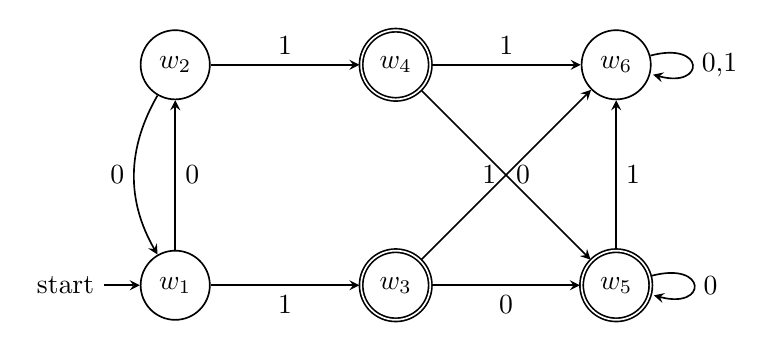
\begin{tikzpicture}[->, >=stealth, node distance=2.8cm, semithick]

  
  \node[state, initial] (w1) {$w_1$};
  \node[state, above of=w1] (w2) {$w_2$};

  \node[state, accepting, right of=w1] (w3) {$w_3$};
  \node[state, accepting, right of=w2] (w4) {$w_4$};

  \node[state, accepting, right of=w3] (w5) {$w_5$};
  \node[state, right of=w4] (w6) {$w_6$};

  
  \path
    (w1) edge[left] node[right]{0} (w2)
    (w2) edge[bend right] node[left]{0} (w1);

  \path
    (w1) edge node[below]{1} (w3)
    (w2) edge node[above]{1} (w4);
 
  \path
    (w3) edge node[below]{0} (w5)
    (w3) edge node[left]{1} (w6);

  \path
    (w4) edge node[right]{0} (w5)
    (w4) edge node[above]{1} (w6);

  \path
    (w5) edge node[right]{1} (w6);
  
  \path
    (w6) edge[loop right] node{0,1} (w6)
    (w5) edge[loop right] node{0} (w5);

\end{tikzpicture}
}
\end {center}


\begin{enumerate}
    \item Step 1: Draw a table of all pair of statess (X,Y).

    
    \begin{center}
    \begin{tabular}{c|cccccc}
        & $w_1$ & $w_2$ & $w_3$ & $w_4$ & $w_5$ & $w_6$ \\ \hline
    $w_1$ & --    &       & \checkmark & \checkmark & \checkmark &       \\
    $w_2$ &       & --    & \checkmark & \checkmark & \checkmark &       \\
    $w_3$ &       &       & --          &            &            & \checkmark \\
    $w_4$ &       &       &             & --          &            & \checkmark \\
    $w_5$ &       &       &             &             & --          & \checkmark \\
    $w_6$ &       &       &             &             &             & --
    \end{tabular}
    \end{center}

    \item step 2: Mark all pairs where $(X \in F \land Y \notin F) \lor (X \notin F \land Y \in F)$
    

    \[
    \begin{array}{l}

    (w_1,w_2)\;
    \left\{
    \begin{array}{l}
    V(w_1,0)=w_2,\quad V(w_2,0)=w_1, \\[4pt]
    V(w_1,1)=w_3,\quad V(w_2,1)=w_4
    \end{array}
    \right.
    \\[12pt]
    \\
    (w_3,w_4)\;
    \left\{
    \begin{array}{l}
    V(w_3,0)=w_5,\quad V(w_4,0)=w_5, \\[4pt]
    V(w_3,1)=w_6,\quad V(w_4,1)=w_6
    \end{array}
    \right.
    \\[12pt]
    \\
    (w_3,w_5)\;
    \left\{
    \begin{array}{l}
    V(w_3,0)=w_5,\quad V(w_5,0)=w_5, \\[4pt]
    V(w_3,1)=w_6,\quad V(w_5,1)=w_6
    \end{array}
    \right.
    \\[12pt]
    \\
    (w_4,w_5)\;
    \left\{
    \begin{array}{l}
    V(w_4,0)=w_5,\quad V(w_5,0)=w_5, \\[4pt]
    V(w_4,1)=w_6,\quad V(w_5,1)=w_6
    \end{array}
    \right.
    \\[12pt]
    \\
    (w_1,w_6)\;
    \left\{
    \begin{array}{l}
    V(w_1,0)=w_2,\quad V(w_6,0)=w_6, \\[4pt]
    V(w_1,1)=w_3,\quad V(w_6,1)=w_6
    \end{array}
    \right.
    \\[12pt]
    \\
    (w_2,w_6)\;
    \left\{
    \begin{array}{l}
    V(w_2,0)=w_1,\quad V(w_6,0)=w_6, \\[4pt]
    V(w_2,1)=w_4,\quad V(w_6,1)=w_6
    \end{array}
    \right.

    \end{array}
    \]

    \item step 3: Iteratively mark pairs where transitions lead to already marked pairs until no new pairs can be marked.
    
    \[\begin{array}{l}
    (w_1,w_2)\;
    \left\{
    \begin{array}{l}
    V(w_1,0)=w_2,\quad V(w_2,0)=w_1, \\[4pt]
    V(w_1,1)=w_3,\quad V(w_2,1)=w_4
    \end{array}
    \right.
    \\[12pt]
    \\
    (w_3,w_4)\;
    \left\{
    \begin{array}{l}
    V(w_3,0)=w_5,\quad V(w_4,0)=w_5, \\[4pt]
    V(w_3,1)=w_6,\quad V(w_4,1)=w_6
    \end{array}
    \right.
    \\[12pt]
    \\
    (w_3,w_5)\;
    \left\{
    \begin{array}{l}
    V(w_3,0)=w_5,\quad V(w_5,0)=w_5, \\[4pt]
    V(w_3,1)=w_6,\quad V(w_5,1)=w_6
    \end{array}
    \right.
    \\[12pt]
    \\
    (w_4,w_5)\;
    \left\{
    \begin{array}{l}
    V(w_4,0)=w_5,\quad V(w_5,0)=w_5, \\[4pt]
    V(w_4,1)=w_6,\quad V(w_5,1)=w_6
    \end{array}
    \right.
    
  \end{array}
    \]

  \item step 4: Combine all the unmarked pairs into equivalence classes.
  
    \[\{w_1,w_2\},\;\{w_3,w_4,w_5\},\;\{w_6\}\]

    Hence the final diagram is:

    \begin{center}
    \fbox{
    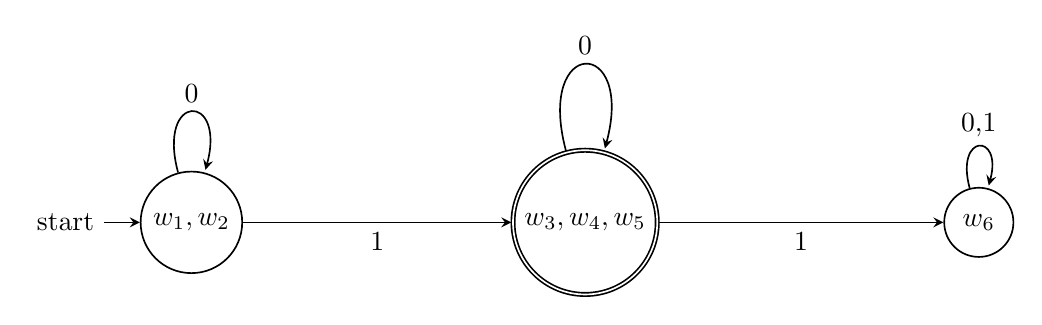
\begin{tikzpicture}[->, >=stealth, node distance=5cm, semithick]

    
    \node[state, initial] (A) {$w_1,w_2$};
    \node[state, accepting, right of=A] (B) {$w_3,w_4,w_5$};
    \node[state, right of=B] (C) {$w_6$};

    \path
        (A) edge[loop above] node{0} (A)
        (A) edge node[below]{1} (B)
        (B) edge[loop above] node{0} (B)
        (B) edge node[below]{1} (C)
        (C) edge[loop above] node{0,1} (C);

    \end{tikzpicture}
    }
    \end{center}


\end{enumerate}


\subsubsection{Subset}


\[L(M_1) \subseteq L(M_2) \leftrightarrow \forall x \in \Sigma^*, \ x \in L(M_1) \to x \in L(M_2)\]

\textbf{Example:}

Let
\[
L(M_1) = \{0^n1^m \mid n \ge 1,\; m \ge 1\}, \qquad
L(M_2) = \{0^n1^m \mid n \ge 0,\; m \ge 0\}.
\]

Since every string accepted by $M_1$ is also accepted by $M_2$, we have
\[
L(M_1) \subseteq L(M_2).
\]

\[
M_1 = (W_1,\Sigma,V_1,S_1,F_1)
\]

where
\[
W_1 = \{w_0,w_1,w_2,w_3\},\quad
\Sigma = \{0,1\},\quad
S_1 = w_0,\quad
F_1 = \{w_2\}.
\]

\begin{center}
\fbox{
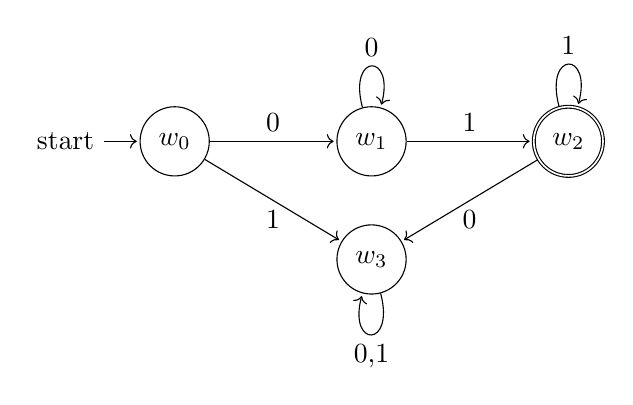
\begin{tikzpicture}[shorten >=1pt, node distance=2.5cm, on grid, auto]

    \node[state, initial] (w0) {$w_0$};
    \node[state] (w1) [right=of w0] {$w_1$};
    \node[state, accepting] (w2) [right=of w1] {$w_2$};
    \node[state] (w3) [below=1.5cm of w1] {$w_3$};

    \path[->]
        (w0) edge node {0} (w1)
        (w1) edge[loop above] node {0} ()
        (w1) edge node {1} (w2)
        (w2) edge[loop above] node {1} ()
        (w0) edge node[below] {1} (w3)
        (w2) edge[below] node {0} (w3)
        (w3) edge[loop below] node {0,1} ();

\end{tikzpicture}
}
\end{center}

\[
M_2 = (W_2,\Sigma,V_2,S_2,F_2)
\]

where
\[
W_2 = \{w_0,w_1,w_2,w_3\},\quad
\Sigma = \{0,1\},\quad
S_2 = w_0,\quad
F_2 = \{w_0,w_1,w_2\}.
\]

\begin{center}
\fbox{
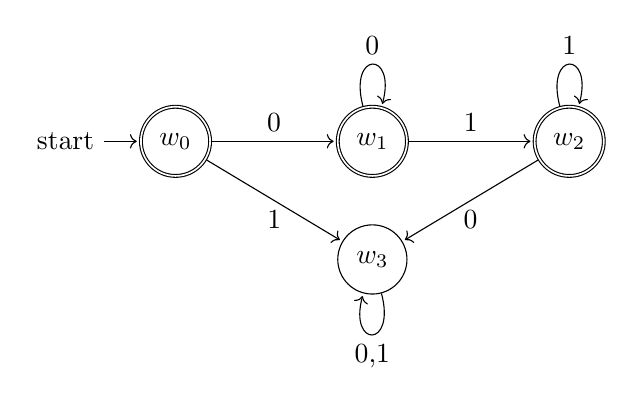
\begin{tikzpicture}[shorten >=1pt, node distance=2.5cm, on grid, auto]

    \node[state, initial, accepting] (w0) {$w_0$};
    \node[state, accepting] (w1) [right=of w0] {$w_1$};
    \node[state, accepting] (w2) [right=of w1] {$w_2$};
    \node[state] (w3) [below=1.5cm of w1] {$w_3$};

    \path[->]
        (w0) edge node {0} (w1)
        (w1) edge[loop above] node {0} ()
        (w1) edge node {1} (w2)
        (w2) edge[loop above] node {1} ()
        (w0) edge node[below] {1} (w3)
        (w2) edge[below] node {0} (w3)
        (w3) edge[loop below] node {0,1} ();

\end{tikzpicture}
}
\end{center}


\subsubsection{Universality}


\[L(M) = \Sigma^* \leftrightarrow \forall x \in \Sigma^*, \ x \in L(M)\]

A DFA $M$ is \textbf{universal} if it accepts all possible strings over the alphabet $\Sigma$.

\textbf{Example:}


Let $ M = (W,\Sigma,V,S,F)$ where


\[
W = \{q_0\},\quad
\Sigma = \{0,1\},\quad
S = q_0,\quad
F = \{q_0\}.
\]

\begin{center}
\fbox{
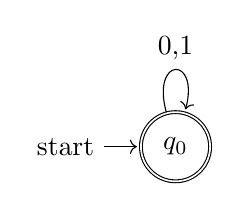
\begin{tikzpicture}[shorten >=1pt, node distance=2.5cm, on grid, auto]

    \node[state, initial, accepting] (q0) {$q_0$};

    \path[->]
        (q0) edge[loop above] node {0,1} ();

\end{tikzpicture}
}
\end{center}

Since $q_0$ is both the initial and only accepting state, and all transitions (on both 0 and 1) loop back to $q_0$, every string over $\{0,1\}$ is accepted. Hence:
\[
L(M) = \Sigma^* = \{\varepsilon, 0, 1, 00, 01, 10, 11, 000, \ldots\}.
\]

\subsection{Closure Properties}

\subsubsection{Union}


\[L(M_1) \cup L(M_2) = \{x \in \Sigma^* \mid x \in L(M_1) \lor x \in L(M_2)\}\]

Given $M_1 = (W_1, \Sigma, V_1, S_1, F_1)$ and $M_2 = (W_2, \Sigma, V_2, S_2, F_2)$, the union is constructed as:
\[M = (W_1 \times W_2, \Sigma, V, (S_1, S_2), F)\]
where
\[F = \{(w_1, w_2) \mid w_1 \in F_1 \lor w_2 \in F_2\}\]
and
\[V((w_1, w_2), a) = (V_1(w_1, a), V_2(w_2, a))\]

\textbf{Example:}

Let $L(M_1)$ be the set of strings over $\{a,b\}$ containing at least one $a$,  
and let $L(M_2)$ be the set of strings containing at least one $b$.

The union language is:
\[
L(M_1) \cup L(M_2) = \{ w \in \{a,b\}^* \mid w \text{ contains at least one } a \text{ or one } b \}.
\]


\begin{enumerate}

\item Component DFA $M_1$: Accepts strings with at least one $a$.

$M_1 = (W_1,\Sigma,V_1,S_1,F_1)$ where

\[
W_1 = \{q_0,q_1\}, \quad
\Sigma = \{a,b\}, \quad
S_1 = q_0, \quad
F_1 = \{q_1\}.
\]

\begin{center}
\fbox{
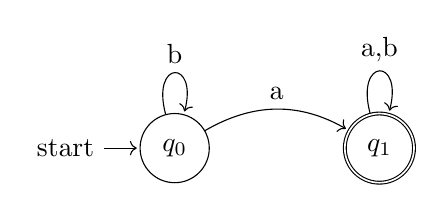
\begin{tikzpicture}[shorten >=1pt, node distance=2.6cm, on grid, auto]

    \node[state, initial] (q0) {$q_0$};
    \node[state, accepting] (q1) [right=of q0] {$q_1$};

    \path[->]
        (q0) edge[bend left] node {a} (q1)
        (q0) edge[loop above] node {b} ()
        (q1) edge[loop above] node {a,b} ();

\end{tikzpicture}
}
\end{center}


\item Component DFA $M_2$: Accepts strings with at least one $b$.

$M_2 = (W_2,\Sigma,V_2,S_2,F_2)$ where

\[
W_2 = \{p_0,p_1\}, \quad
\Sigma = \{a,b\}, \quad
S_2 = p_0, \quad
F_2 = \{p_1\}.
\]

\begin{center}
\fbox{
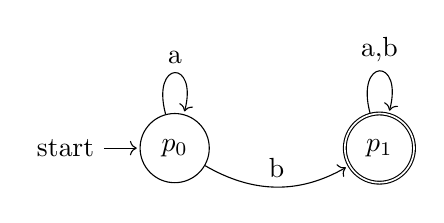
\begin{tikzpicture}[shorten >=1pt, node distance=2.6cm, on grid, auto]

    \node[state, initial] (p0) {$p_0$};
    \node[state, accepting] (p1) [right=of p0] {$p_1$};

    \path[->]
        (p0) edge[bend right] node {b} (p1)
        (p0) edge[loop above] node {a} ()
        (p1) edge[loop above] node {a,b} ();

\end{tikzpicture}
}
\end{center}


Union Construction: 

\[
M = M_1 \cup M_2 = (W_1 \times W_2,\ \Sigma,\ V,\ (q_0,p_0),\ F)
\]
where
\[
W = \{(q_0,p_0), (q_0,p_1), (q_1,p_0), (q_1,p_1)\}
\]
and
\[
F = \{(x,y) \mid x \in F_1 \lor y \in F_2\} = \{(q_1,p_0), (q_0,p_1), (q_1,p_1)\}.
\]

\begin{center}
\fbox{
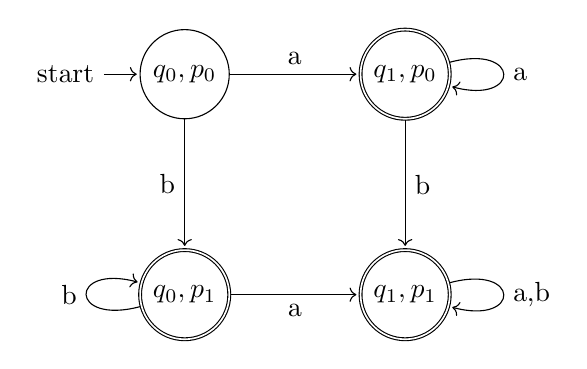
\begin{tikzpicture}[shorten >=1pt, node distance=2.8cm, on grid, auto]

    \node[state, initial] (00) {$q_0,p_0$};
    \node[state, accepting] (10) [right=of 00] {$q_1,p_0$};
    \node[state, accepting] (01) [below=of 00] {$q_0,p_1$};
    \node[state, accepting] (11) [right=of 01] {$q_1,p_1$};

    \path[->]
        (00) edge node[above] {a} (10)
        (00) edge node[left] {b} (01)

        (10) edge node[right] {b} (11)
        (10) edge[loop right] node {a} ()
        
        (01) edge node[below] {a} (11)
        (01) edge[loop left] node {b} ()
        
        (11) edge[loop right] node {a,b} ();

\end{tikzpicture}
}
\end{center}

The product state $(q_i, p_j)$ represents ``$M_1$ in state $q_i$ and $M_2$ in state $p_j$". A state is accepting if \emph{either} component is in an accepting state (union semantics).

Thus,
\[
L(M_1) \cup L(M_2) = L(M) = \{w \in \{a,b\}^* \mid w \neq \varepsilon\}.
\]

Verification:

\begin{enumerate}
    \item $\varepsilon$: Neither $M_1$ nor $M_2$ accepts $\to$ rejected 
    \item $a$: $M_1$ accepts $\to$ accepted 
    \item $b$: $M_2$ accepts $\to$ accepted 
    \item $ab$: Both accept $\to$ accepted 
\end{enumerate}

\end{enumerate}

\subsubsection{Intersection}

\[L(M_1) \cap L(M_2) = \{x \in \Sigma^* \mid x \in L(M_1) \land x \in L(M_2)\}\]

Given $M_1 = (W_1, \Sigma, V_1, S_1, F_1)$ and $M_2 = (W_2, \Sigma, V_2, S_2, F_2)$, the intersection is constructed as:
\[M = (W_1 \times W_2, \Sigma, V, (S_1, S_2), F)\]
where
\[F = \{(w_1, w_2) \mid w_1 \in F_1 \land w_2 \in F_2\}\]
and
\[V((w_1, w_2), a) = (V_1(w_1, a), V_2(w_2, a))\]

\textbf{Example:}

Let $L(M_1)$ be the set of strings over $\{a,b\}$ containing at least one $a$,  
and let $L(M_2)$ be the set of strings containing at least one $b$.

The intersection language is:
\[
L(M_1) \cap L(M_2) = \{ w \in \{a,b\}^* \mid w \text{ contains at least one } a \text{ and at least one } b \}.
\]


\begin{enumerate}

\item Component DFA $M_1$: Accepts strings with at least one $a$.

$M_1 = (W_1,\Sigma,V_1,S_1,F_1)$ where

\[
W_1 = \{q_0,q_1\}, \quad
\Sigma = \{a,b\}, \quad
S_1 = q_0, \quad
F_1 = \{q_1\}.
\]

\begin{center}
\fbox{
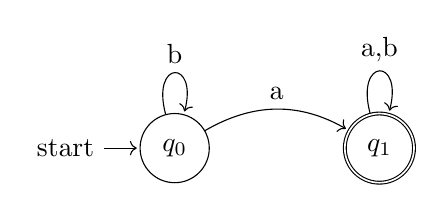
\begin{tikzpicture}[shorten >=1pt, node distance=2.6cm, on grid, auto]

    \node[state, initial] (q0) {$q_0$};
    \node[state, accepting] (q1) [right=of q0] {$q_1$};

    \path[->]
        (q0) edge[bend left] node {a} (q1)
        (q0) edge[loop above] node {b} ()
        (q1) edge[loop above] node {a,b} ();

\end{tikzpicture}
}
\end{center}


\item Component DFA $M_2$: Accepts strings with at least one $b$.

$M_2 = (W_2,\Sigma,V_2,S_2,F_2)$ where

\[
W_2 = \{p_0,p_1\}, \quad
\Sigma = \{a,b\}, \quad
S_2 = p_0, \quad
F_2 = \{p_1\}.
\]

\begin{center}
\fbox{
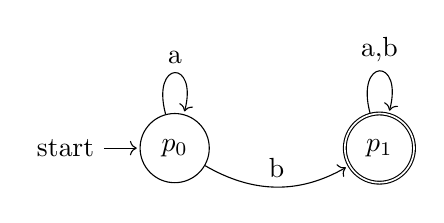
\begin{tikzpicture}[shorten >=1pt, node distance=2.6cm, on grid, auto]

    \node[state, initial] (p0) {$p_0$};
    \node[state, accepting] (p1) [right=of p0] {$p_1$};

    \path[->]
        (p0) edge[bend right] node {b} (p1)
        (p0) edge[loop above] node {a} ()
        (p1) edge[loop above] node {a,b} ();

\end{tikzpicture}
}
\end{center}


Intersection construction:

\[
M = M_1 \cap M_2 = (W_1 \times W_2,\ \Sigma,\ V,\ (q_0,p_0),\ F)
\]
where
\[
W = \{(q_0,p_0), (q_0,p_1), (q_1,p_0), (q_1,p_1)\}
\]
and
\[
F = \{(x,y) \mid x \in F_1 \land y \in F_2\} = \{(q_1,p_1)\}.
\]

\begin{center}
\fbox{
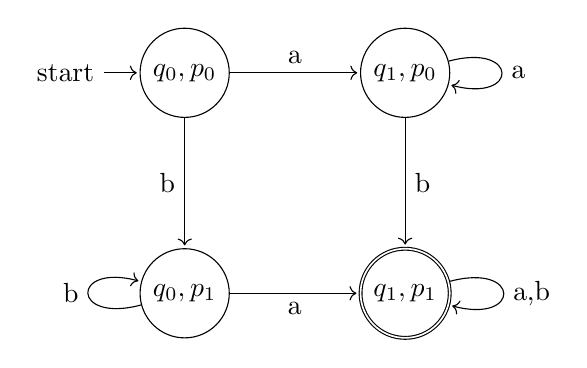
\begin{tikzpicture}[shorten >=1pt, node distance=2.8cm, on grid, auto]

    \node[state, initial] (00) {$q_0,p_0$};
    \node[state] (10) [right=of 00] {$q_1,p_0$};
    \node[state] (01) [below=of 00] {$q_0,p_1$};
    \node[state, accepting] (11) [right=of 01] {$q_1,p_1$};

    \path[->]
        (00) edge node[above] {a} (10)
        (00) edge node[left] {b} (01)

        (10) edge node[right] {b} (11)
        (10) edge[loop right] node {a} ()

        (01) edge node[below] {a} (11)
        (01) edge[loop left] node {b} ()

        (11) edge[loop right] node {a,b} ();

\end{tikzpicture}
}
\end{center}

The product state $(q_i, p_j)$ represents ``$M_1$ in state $q_i$ and $M_2$ in state $p_j$". A state is accepting if \emph{both} components are in accepting states (intersection semantics).

Thus,
\[
L(M_1) \cap L(M_2) = L(M) = \{w \in \{a,b\}^* \mid w \text{ contains both } a \text{ and } b\}.
\]

Verification:

\begin{enumerate}
    \item $\varepsilon$: Neither contains $a$ nor $b$ $\to$ rejected 
    \item $a$: Contains $a$ but not $b$ $\to$ rejected 
    \item $b$: Contains $b$ but not $a$ $\to$ rejected 
    \item $ab$: Contains both $a$ and $b$ $\to$ accepted 
    \item $ba$: Contains both $a$ and $b$ $\to$ accepted 
    \item $aabb$: Contains both $a$ and $b$ $\to$ accepted 
\end{enumerate}

\end{enumerate}

\subsubsection{Complement}

\[L(M)^c = \Sigma^* \setminus L(M) = \{x \in \Sigma^* \mid x \notin L(M)\}\]

Given $M = (W, \Sigma, V, S, F)$, the complement is constructed as:
\[M^c = (W, \Sigma, V, S, F^c)\]
where
\[F^c = W \setminus F\]

The complement DFA has the same structure but with accepting and non-accepting states swapped.

\textbf{Example:}

Let $L(M_1)$ be the set of strings over $\{a,b\}$ that contain at least one $a$.
The complement language is:

\[
L(M_1)^c = \{ w \in \{a,b\}^* \mid w \text{ contains no } a \}
        = b^*.
\]



Original DFA $M_1$: Accepts strings with at least one $a$.

$M_1 = (W,\Sigma,V,S,F)$ where

\[
W = \{q_0,q_1\}, \quad
\Sigma = \{a,b\}, \quad
S = q_0, \quad
F = \{q_1\}.
\]

\begin{center}
\fbox{
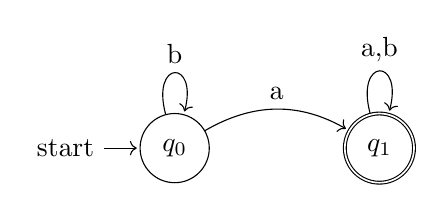
\begin{tikzpicture}[shorten >=1pt, node distance=2.6cm, on grid, auto]

    \node[state, initial] (q0) {$q_0$};
    \node[state, accepting] (q1) [right=of q0] {$q_1$};

    \path[->]
        (q0) edge[bend left] node {a} (q1)
        (q0) edge[loop above] node {b} ()
        (q1) edge[loop above] node {a,b} ();

\end{tikzpicture}
}
\end{center}


Complement Construction:

\[
M_1^c = (W,\Sigma,V,S,F^c)
\]
where
\[
F^c = W \setminus F = \{q_0,q_1\} \setminus \{q_1\} = \{q_0\}.
\]

\begin{center}
\fbox{
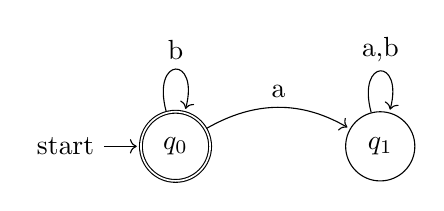
\begin{tikzpicture}[shorten >=1pt, node distance=2.6cm, on grid, auto]

    \node[state, initial, accepting] (q0c) {$q_0$};
    \node[state] (q1c) [right=of q0c] {$q_1$};

    \path[->]
        (q0c) edge[bend left] node {a} (q1c)
        (q0c) edge[loop above] node {b} ()
        (q1c) edge[loop above] node {a,b} ();

\end{tikzpicture}
}
\end{center}

The complement DFA accepts all strings that the original rejects, and vice versa. State $q_0$ (previously non-accepting) is now accepting, while state $q_1$ (previously accepting) is now non-accepting.

Thus,
\[
L(M_1)^c = L(M_1^c) = b^* = \{\varepsilon, b, bb, bbb, \ldots\}.
\]

Verification:

\begin{enumerate}
    \item $\varepsilon$: No $a$ $\to$ accepted 
    \item $b$: No $a$ $\to$ accepted 
    \item $a$: Contains $a$ $\to$ rejected 
    \item $ab$: Contains $a$ $\to$ rejected 
    \item $bbb$: No $a$ $\to$ accepted 
\end{enumerate}

\subsubsection{Difference}

\[L(M_1) - L(M_2) = \{x \in \Sigma^* \mid x \in L(M_1) \land x \notin L(M_2)\}\]

The difference is constructed using intersection with complement:
\[L(M_1) - L(M_2) = L(M_1) \cap L(M_2)^c\]

Given $M_1 = (W_1, \Sigma, V_1, S_1, F_1)$ and $M_2 = (W_2, \Sigma, V_2, S_2, F_2)$:
\begin{enumerate}
    \item First, construct $M_2^c = (W_2, \Sigma, V_2, S_2, F_2^c)$ where $F_2^c = W_2 \setminus F_2$
    \item Then, construct the product: $M = (W_1 \times W_2, \Sigma, V, (S_1, S_2), F)$ where
    \[F = \{(w_1, w_2) \mid w_1 \in F_1 \land w_2 \in F_2^c\}\]
\end{enumerate}

\textbf{Example:}

Let $L(M_1)$ be the set of strings over $\{a,b\}$ that contain at least one $a$,  
and let $L(M_2)$ be the set of strings that contain at least one $b$.

The difference language is:
\[
L(M_1) - L(M_2)
  = \{ w \in \{a,b\}^* \mid w \text{ contains at least one } a \text{ and contains no } b \}
  = a^+.
\]



\begin{enumerate}

\item Component DFA $M_1$: Accepts strings with at least one $a$.

$M_1 = (W_1,\Sigma,V_1,S_1,F_1)$ where

\[
W_1 = \{q_0,q_1\}, \quad
\Sigma = \{a,b\}, \quad
S_1 = q_0, \quad
F_1 = \{q_1\}.
\]

\begin{center}
\fbox{
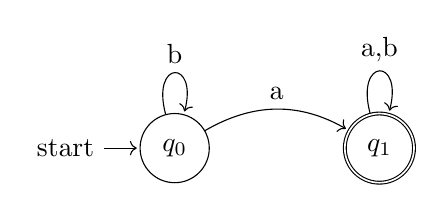
\begin{tikzpicture}[shorten >=1pt, node distance=2.6cm, on grid, auto]

    \node[state, initial] (q0) {$q_0$};
    \node[state, accepting] (q1) [right=of q0] {$q_1$};

    \path[->]
        (q0) edge[bend left] node {a} (q1)
        (q0) edge[loop above] node {b} ()
        (q1) edge[loop above] node {a,b} ();

\end{tikzpicture}
}
\end{center}


\item Component DFA $M_2$: Accepts strings with at least one $b$.

$M_2 = (W_2,\Sigma,V_2,S_2,F_2)$ where

\[
W_2 = \{p_0,p_1\}, \quad
\Sigma = \{a,b\}, \quad
S_2 = p_0, \quad
F_2 = \{p_1\}.
\]

\begin{center}
\fbox{
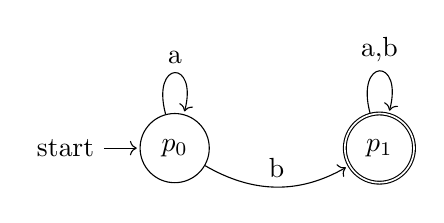
\begin{tikzpicture}[shorten >=1pt, node distance=2.6cm, on grid, auto]

    \node[state, initial] (p0) {$p_0$};
    \node[state, accepting] (p1) [right=of p0] {$p_1$};

    \path[->]
        (p0) edge[bend right] node {b} (p1)
        (p0) edge[loop above] node {a} ()
        (p1) edge[loop above] node {a,b} ();

\end{tikzpicture}
}
\end{center}


Difference Construction:

First, construct the complement of $M_2$:
\[
M_2^c = (W_2,\Sigma,V_2,S_2,F_2^c)
\quad\text{where}\quad
F_2^c = W_2 \setminus F_2 = \{p_0,p_1\} \setminus \{p_1\} = \{p_0\}.
\]

Then construct the product automaton:

\[
M = M_1 - M_2 = (W_1 \times W_2,\ \Sigma,\ V,\ (q_0,p_0),\ F)
\]
where
\[
W = \{(q_0,p_0), (q_0,p_1), (q_1,p_0), (q_1,p_1)\}
\]
and
\[
F = \{(x,y) \mid x \in F_1 \land y \in F_2^c\} = \{(q_1,p_0)\}.
\]

\begin{center}
\fbox{
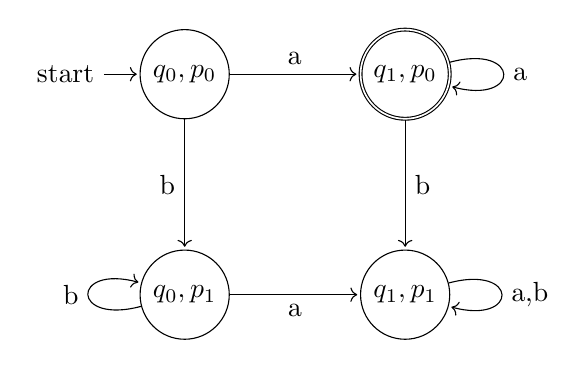
\begin{tikzpicture}[shorten >=1pt, node distance=2.8cm, on grid, auto]

    \node[state, initial] (00) {$q_0,p_0$};
    \node[state, accepting] (10) [right=of 00] {$q_1,p_0$};
    \node[state] (01) [below=of 00] {$q_0,p_1$};
    \node[state] (11) [right=of 01] {$q_1,p_1$};

    \path[->]
        (00) edge node[above] {a} (10)
        (00) edge node[left] {b} (01)

        (10) edge[loop right] node {a} ()
        (10) edge node[right] {b} (11)

        (01) edge node[below] {a} (11)
        (01) edge[loop left] node {b} ()

        (11) edge[loop right] node {a,b} ();

\end{tikzpicture}
}
\end{center}

The product state $(q_i, p_j)$ represents ``$M_1$ in state $q_i$ and $M_2^c$ in state $p_j$". Only state $(q_1, p_0)$ is accepting because it represents strings where $M_1$ accepts (contains $a$) AND $M_2^c$ accepts (contains no $b$).

Thus,
\[
L(M_1) - L(M_2) = L(M) = a^+ = \{a, aa, aaa, \ldots\}.
\]

Verification:

\begin{enumerate}
    \item $\varepsilon$: No $a$ $\to$ rejected 
    \item $a$: Contains $a$, no $b$ $\to$ accepted 
    \item $b$: Contains $b$ $\to$ rejected 
    \item $ab$: Contains $b$ $\to$ rejected 
    \item $aaa$: Contains $a$, no $b$ $\to$ accepted 
\end{enumerate}

\end{enumerate}

\subsubsection{Concatenation}

\[L(M_1) \cdot L(M_2) = \{xy \mid x \in L(M_1) \land y \in L(M_2)\}\]

Given DFAs $M_1 = (W_1, \Sigma, V_1, S_1, F_1)$ and $M_2 = (W_2, \Sigma, V_2, S_2, F_2)$, concatenation requires constructing an NFA (with $\varepsilon$-transitions):

\[M = M_1 \cdot M_2 = (W_1 \cup W_2,\ \Sigma,\ V,\ S_1,\ F_2)\]

where the transition function $\delta$ includes:
\begin{enumerate}
    \item All transitions from $M_1$: $\delta(q, a) = V_1(q, a)$ for $q \in W_1$
    \item All transitions from $M_2$: $\delta(q, a) = V_2(q, a)$ for $q \in W_2$
    \item $\varepsilon$-transitions from every accepting state of $M_1$ to the start state of $M_2$:
    \[V(f, \varepsilon) = S_2 \text{ for all } f \in F_1\]
\end{enumerate}

\textbf{Example:}

Let $L(M_1)$ be the set of strings over $\{x,y\}$ that contain at least one $x$,  
and let $L(M_2)$ be the set of strings over $\{x,y\}$ that contain at least one $y$.

The concatenation language is:
\[
L(M_1) \cdot L(M_2)
 = \{ uv \mid u \in L(M_1),\ v \in L(M_2) \}
\]

This represents all strings that can be split into two parts: the first part contains at least one $x$, and the second part contains at least one $y$.



\begin{enumerate}

\item Component DFA $M_1$: Accepts strings with at least one $x$.

$M_1 = (W_1,\Sigma,V_1,S_1,F_1)$ where

\[
W_1 = \{q_0,q_1\}, \quad
\Sigma = \{x,y\}, \quad
S_1 = q_0, \quad
F_1 = \{q_1\}.
\]

\begin{center}
\fbox{
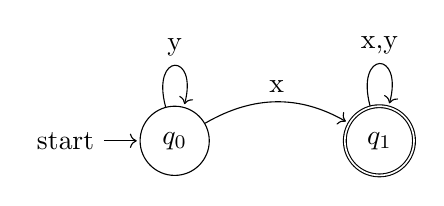
\begin{tikzpicture}[shorten >=1pt, node distance=2.6cm, on grid, auto]

    \node[state, initial] (q0) {$q_0$};
    \node[state, accepting] (q1) [right=of q0] {$q_1$};

    \path[->]
        (q0) edge[bend left] node {x} (q1)
        (q0) edge[loop above] node {y} ()
        (q1) edge[loop above] node {x,y} ();

\end{tikzpicture}
}
\end{center}



\item Component DFA $M_2$: Accepts strings with at least one $y$.

$M_2 = (W_2,\Sigma,V_2,S_2,F_2)$ where

\[
W_2 = \{p_0,p_1\}, \quad
\Sigma = \{x,y\}, \quad
S_2 = p_0, \quad
F_2 = \{p_1\}.
\]

\begin{center}
\fbox{
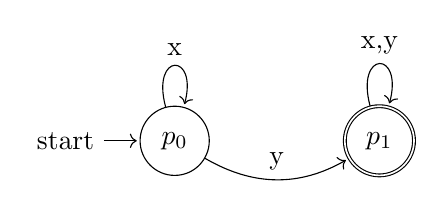
\begin{tikzpicture}[shorten >=1pt, node distance=2.6cm, on grid, auto]

    \node[state, initial] (p0) {$p_0$};
    \node[state, accepting] (p1) [right=of p0] {$p_1$};

    \path[->]
        (p0) edge[bend right] node {y} (p1)
        (p0) edge[loop above] node {x} ()
        (p1) edge[loop above] node {x,y} ();

\end{tikzpicture}
}
\end{center}



Concatenation Construction (NFA):

\[
M = M_1 \cdot M_2 = (W_1 \cup W_2,\ \Sigma,\ V,\ q_0,\ F_2)
\]

where $W = \{q_0, q_1, p_0, p_1\}$, start state is $q_0$, accepting states are $F = \{p_1\}$, and the $\varepsilon$-transition is:
\[
q_1 \xrightarrow{\varepsilon} p_0
\]

\begin{center}
\fbox{
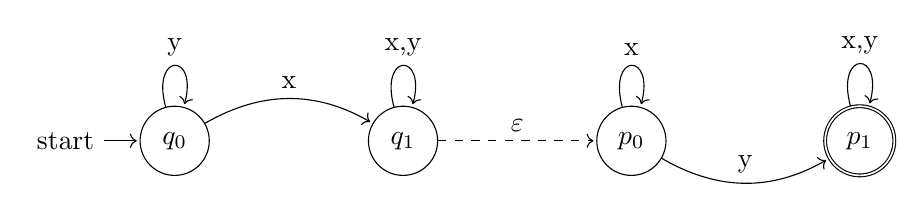
\begin{tikzpicture}[shorten >=1pt, node distance=2.9cm, on grid, auto]

    
    \node[state, initial] (q0) {$q_0$};
    \node[state] (q1) [right=of q0] {$q_1$};

    
    \node[state] (p0) [right=of q1] {$p_0$};
    \node[state, accepting] (p1) [right=of p0] {$p_1$};

    
    \path[->]
        (q0) edge[bend left] node {x} (q1)
        (q0) edge[loop above] node {y} ()
        (q1) edge[loop above] node {x,y} ();

    
    \path[->]
        (q1) edge[dashed] node {$\varepsilon$} (p0);

    
    \path[->]
        (p0) edge[bend right] node {y} (p1)
        (p0) edge[loop above] node {x} ()
        (p1) edge[loop above] node {x,y} ();

\end{tikzpicture}
}
\end{center}

The $\varepsilon$-transition allows the NFA to non-deterministically ``jump" from the accepting state of $M_1$ to the start state of $M_2$, effectively concatenating the two languages.

Thus,
\[
L(M_1 \cdot M_2) = L(M_1)L(M_2).
\]

Verification:

\begin{enumerate}
    \item $xy$: First part $x \in L(M_1)$, second part $y \in L(M_2)$ $\to$ accepted 
    \item $xxy$: First part $xx \in L(M_1)$, second part $y \in L(M_2)$ $\to$ accepted 
    \item $xyy$: First part $x \in L(M_1)$, second part $yy \in L(M_2)$ $\to$ accepted 
    \item $xxyy$: Multiple valid splits $\to$ accepted 
    \item $x$: No part with $y$ $\to$ rejected 
    \item $y$: No part with $x$ $\to$ rejected 
\end{enumerate}

Unlike the previous closure properties (union, intersection, complement, difference), concatenation requires an NFA with $\varepsilon$-transitions. DFAs alone cannot directly construct concatenation, though the resulting NFA can be converted to a DFA using standard NFA-to-DFA conversion.

\end{enumerate}

\subsubsection{Kleene Star}

\textbf{Example:}

Let $L(M_1)$ be the set of strings over $\{p,q\}$ that contain at least one $p$.

The Kleene star language is:
\[
L(M_1)^* = \{ w_1 w_2 \cdots w_k \mid k \ge 0,\ \forall i,\ w_i \in L(M_1) \}.
\]

Since each $w_i$ must contain at least one $p$, any string in $L(M_1)^*$ is a concatenation of blocks each containing a $p$.

\[
L(M_1)^* = \{p,q\}^* \setminus \{q^n \mid n \ge 1\}.
\]


\begin{enumerate}

\item $M_1 = (W_1,\Sigma,V_1,S_1,F_1)$

\[
W_1 = \{w_0,w_1\}, \quad
\Sigma = \{p,q\}, \quad
S_1 = w_0, \quad
F_1 = \{w_1\}.
\]

\begin{center}
\fbox{
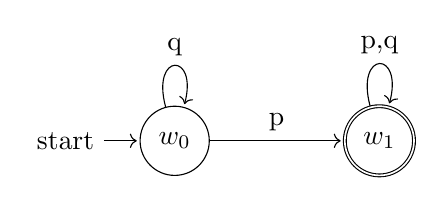
\begin{tikzpicture}[shorten >=1pt, node distance=2.6cm, on grid, auto]

    \node[state, initial] (w0) {$w_0$};
    \node[state, accepting] (w1) [right=of w0] {$w_1$};

    \path[->]
        (w0) edge[left] node [above]{p} (w1)
        (w0) edge[loop above] node {q} ()
        (w1) edge[loop above] node {p,q} ();

\end{tikzpicture}
}
\end{center}



To build $M_1^*$, we create a new start/accepting state $s$ and add:

\[
s \xrightarrow{\varepsilon} S_1,\qquad
F_1 \xrightarrow{\varepsilon} S_1.
\]

So the NFA is:
\[
M_1^* = (W_1 \cup \{s\},\ \Sigma,\ V,\ s,\ F_1 \cup \{s\}).
\]

\begin{center}
\fbox{
\begin{tikzpicture}[shorten >=1pt, node distance=2.4cm, on grid, auto]

    
    \node[state, initial, accepting] (s) {$s$};

    
    \node[state] (w0c) [right=of s] {$w_0$};
    \node[state, accepting] (w1c) [right=of w0c] {$w_1$};

    
    \path[->]
        (w0c) edge[bend left] node {p} (w1c)
        (w0c) edge[loop above] node {q} ()
        (w1c) edge[loop above] node {p,q} ();

    
    \path[->]
        (s) edge node {$\varepsilon$} (w0c)
        (w1c) edge[bend left] node {$\varepsilon$} (w0c);

\end{tikzpicture}
}
\end{center}

Thus,

\[
L(M_1)^* = L(M_1^*).
\]

\end{enumerate}

\subsubsection{Reversal}

\textbf{Example:}

Let $L(M_1)$ be the set of strings over $\{s,a\}$ that end with symbol $a$.

The reversal language is:
\[
L(M_1)^R = \{ w^R \mid w \in L(M_1) \}.
\]
Since $w$ ends with $a$, the reversed string $w^R$ must begin with $a$.

Thus,

\[
L(M_1)^R = \{a\{s,a\}^*\}.
\]



\begin{enumerate}

\item $M_1 = (W_1,\Sigma,V_1,S_1,F_1)$

\[
W_1 = \{w_0,w_1,w_2\}, \quad
\Sigma = \{s,a\}, \quad
S_1 = w_0, \quad
F_1 = \{w_2\}.
\]

\begin{center}
\fbox{
\begin{tikzpicture}[shorten >=1pt, on grid, auto]

    
    \node[state, initial]         (w0) at (0,0)   {$w_0$};
    \node[state]                  (w1) at (3,0)   {$w_1$};
    \node[state, accepting]       (w2) at (6,0)   {$w_2$};

    \path[->]
        (w0) edge node {s} (w1)
        (w0) edge[bend right=30] node[below] {a} (w2)

        (w1) edge[left=15] node[above] {a} (w2)
        (w1) edge[loop above] node {s} ()

        (w2) edge[loop above] node {s,a} ();

\end{tikzpicture}
}
\end{center}



To construct $M_1^R$:

\begin{enumerate}
    \item Reverse all transitions.
    \item Make original final states into the new start states.
    \item Make the original start state the only accepting state.
    \item Because multiple $\varepsilon$-entries may arise, the construction yields an NFA.
\end{enumerate}

Hence,

\[
M_1^R = (W_1,\ \Sigma,\ V^R,\ F_1,\ \{S_1\}).
\]

Where $V^R$ is the reverse of $V_1$.

\begin{center}
\fbox{
\begin{tikzpicture}[shorten >=1pt, on grid, auto]

    
    \node[state, accepting]  (r0) at (0,0)   {$w_0$};
    \node[state]             (r1) at (3,1.5) {$w_1$};
    \node[state, initial right]    (r2) at (6,0)   {$w_2$};

    \path[->]
        
        (r2) edge[left=15] node [above]{a} (r1)
        (r2) edge[bend left=30] node[below] {a} (r0)
        (r2) edge[loop above] node {s,a} ()

        
        (r1) edge[left=15] node [above]{s} (r0)
        (r1) edge[loop above] node {s} ();

\end{tikzpicture}
}
\end{center}


Therefore,

\[
L(M_1)^R = L(M_1^R).
\]

\end{enumerate}

\subsubsection{Homomorphism}

\textbf{Example:}

Let $L(M_1)$ be the set of strings over $\{0,1\}$ that contain at least one $1$:

\[ L(M_1) = \{ w \in \{0,1\}^* \mid w \text{ contains at least one } 1 \}. \]

Define a homomorphism $h$:

\[ h(0) = 01, \quad h(1) = 1. \]

Then the homomorphic image of $L(M_1)$ is:

\[ h(L(M_1)) = \{ h(w) \mid w \in L(M_1) \}. \]


Let

$M_1 = (W_1, \Sigma, V_1, S_1, F_1)$
\[ W_1 = \{w_0,w_1\}, \quad \Sigma = \{0,1\}, \quad S_1 = w_0, \quad F_1 = \{w_1\}. \]

\begin{center}
\fbox{
\begin{tikzpicture}[shorten >=1pt, node distance=2.6cm, on grid, auto]
\node[state, initial] (w0) {$w_0$}; 
\node[state, accepting] (w1) [right=of w0] {$w_1$};
\path[->] 
    (w0) edge[left] node[above] {1} (w1) 
    (w0) edge[loop above] node {0} () 
    (w1) edge[loop above] node {0,1} ();
\end{tikzpicture}
}
\end{center}


The homomorphism $h$ transforms each $0$ into $01$, and each $1$ into $1$. For example:
\[ w = 0101 \in L(M_1) \to h(w) = 01\cdot 01\cdot 1\cdot 1 = 010111 \in h(L(M_1)). \]

Hence,

\[ h(L(M_1)) \text{ is regular.} \]

\subsubsection{Inverse Homomorphism}

\textbf{Example:}

Let $L(M_2)$ be the set of strings over $\{0,1\}$ that start with $1$:

\[ L(M_2) = \{ w \in \{0,1\}^* \mid w \text{ starts with } 1 \}. \]

Define a homomorphism $h$:

\[ h(0) = 01, \quad h(1) = 1. \]

The inverse homomorphic image of $L(M_2)$ is:

\[ h^{-1}(L(M_2)) = \{ w \in \{0,1\}^* \mid h(w) \in L(M_2) \}. \]


Let

$M_2 = (W_2, \Sigma, V_2, S_2, F_2)$
\[ W_2 = \{q_0,q_1\}, \quad \Sigma = \{0,1\}, \quad S_2 = q_0, \quad F_2 = \{q_1\}. \]

\begin{center}
\fbox{
\begin{tikzpicture}[shorten >=1pt, node distance=2.6cm, on grid, auto]
\node[state, initial] (q0) {$q_0$}; 
\node[state, accepting] (q1) [right=of q0] {$q_1$};
\path[->] 
    (q0) edge[left] node [above]{1} (q1) 
    (q0) edge[loop above] node {0} () 
    (q1) edge[loop above] node {0,1} ();
\end{tikzpicture}
}
\end{center}


The inverse homomorphism $h^{-1}$ gives the set of strings $w$ such that $h(w)$ starts with $1$. For instance:

\[ w = 0 \to h(0) = 01 \notin L(M_2) \to 0 \notin h^{-1}(L(M_2)), \]
\[ w = 1 \to h(1) = 1 \in L(M_2) \to 1 \in h^{-1}(L(M_2)). \]

Thus,

\[ h^{-1}(L(M_2)) \text{ is regular.} \]

\subsubsection{Substitution}

\textbf{Example:}

Let $L(M_3)$ be the set of strings over $\{0,1\}$ that contain exactly one $1$:

\[ L(M_3) = \{ w \in \{0,1\}^* \mid w \text{ contains exactly one } 1 \}. \]

Define a substitution $\phi$:

\[ \phi(0) = \{0,00\}, \quad \phi(1) = \{1,11\}. \]

The substitution of $L(M_3)$ is:

\[ \phi(L(M_3)) = \bigcup_{w \in L(M_3)} \phi(w), \]

where $\phi(w)$ replaces each symbol $x$ in $w$ by a string from $\phi(x)$.


Let

$M_3 = (W_3, \Sigma, V_3, S_3, F_3)$

\[ W_3 = \{p_0,p_1,p_2\}, \quad \Sigma = \{0,1\}, \quad S_3 = p_0, \quad F_3 = \{p_2\}. \]

\begin{center}
\fbox{
\begin{tikzpicture}[shorten >=1pt, node distance=2.6cm, on grid, auto]
\node[state, initial] (p0) {$p_0$}; 
\node[state] (p1) [right=of p0] {$p_1$}; 
\node[state, accepting] (p2) [right=of p1] {$p_2$};
\path[->] 
    (p0) edge node {1} (p1) 
    (p0) edge[loop above] node {0} () 
    (p1) edge node {0} (p2) 
    (p2) edge[loop above] node {0,1} ();
\end{tikzpicture}
}
\end{center}


The substitution allows each $0$ to be replaced by $0$ or $00$, and each $1$ by $1$ or $11$, producing a regular language:
\[ \phi(L(M_3)) \text{ is regular.} \]

\section{Pumping Lemma}

For any regular language $L$, there exists a constant $p \geq 1$ (called the pumping length) such that for any string $w \in L$ with $|w| \geq p$, there exists a decomposition $w = xyz$ satisfying:

\[|y| > 0, \ |xy| \leq p, \ \forall i \geq 0, \ xy^iz \in L\]


\textbf{Example:}

Let 

\[A = \{a^n b^n \mid n \geq 0\} \ \text{is not regular}\]

\textit{Proof}

Assume $A$ is regular. Let $p$ be the pumping length. 
Consider $w = a^p b^p \in A$ with $|w| = 2p \geq p$. 
By the Pumping Lemma, $w = xyz$ where $|y| > 0$, $|xy| \leq p$, and $\forall i \geq 0, xy^iz \in A$. 
Since $|xy| \leq p$, both $x$ and $y$ consist only of $a$'s. Let $y = a^k$ where $k > 0$. 
Pump with $i = 2$: $xy^2z = a^{p+k}b^p$. Since $k > 0$, we have $p + k > p$, so $xy^2z \notin A$. Contradiction. Therefore, $A$ is not regular. \qed

\textbf{Intuitively:}

Suppose $p = 7$. Consider $w = a^7b^7$ where $|xy| \leq 7$. There are three cases for where $y$ can be located:

\begin{enumerate}
    \item $y$ is in the $a$ part.
    
    Let $w = \underbrace{aa}_x \underbrace{aaaa}_y \underbrace{ab^7}_z$.

    Pumping with $i = 2$: $xy^2z = a^{11}b^7 \notin A$ since $11 \neq 7$. 
    
    
    \item $y$ is in the $b$ part.
    
    Let $w = \underbrace{a^7}_x \underbrace{bb}_y \underbrace{b^5}_z$.
    
    Pumping with $i = 2$: $xy^2z = a^7b^{9} \notin A$ since $7 \neq 9$. 
    
    
    \item $y$ spans both $a$ and $b$ parts.
    
    Let $w = \underbrace{aaaa}_x \underbrace{aaab}_y \underbrace{b^6}_z$.
    
    Pumping with $i = 2$: $xy^2z = aaaaaaabaabb^6 \notin A$ (wrong pattern for $a^nb^n$). 
\end{enumerate}

Since $|xy| \leq p = 7$, all cases lead to contradiction. Therefore, $A$ is not regular.

\section{Regular Grammar}

Formally

\[
G = (V, T, S, P)
\]

where:

\begin{enumerate}
    \item $V$ = a finite set of variables (nonterminal symbols),
    \item $T$ = a finite set of terminal symbols,
    \item $S$ = the start symbol $(S \in V)$,
    \item $P$ = the set of production rules for terminals and nonterminals.
\end{enumerate}


\textbf{In general:}

Let 

\[
G = (\{f, g, h\},\ \{0,1\},\ f,\ \{f \to gh,\ g \to 0,\ h \to 1\})
\]

where

\begin{align*}
V &= \{f, g, h\} \qquad & T &= \{0, 1\},\\
S &= f               \qquad & P &= \{\,f \to gh,\ g \to 0,\ h \to 1\,\}.
\end{align*}


From this we can derive 

\[
\begin{aligned}
f &\to gh \\
  &\to 0h \\
  &\to 01
\end{aligned}
\]

Hence, we can coclude, \[\fbox{L(G) = \{10\}}\]

\section{Context-Free Grammar and Language}

Formally, a context-free grammar is \(G=(V,\Sigma,R,S)\) where

\begin{enumerate}
    \item $V$ is the set of nonterminals.
    \item $\Sigma$ is the set of terminals.
    \item $S \in V$ is the start symbol.
    \item $R \subseteq V \times (V \cup \Sigma)^*$ is the set of productions, each of the form
    $A \to \alpha$ with $A \in V$ and $\alpha \in (V \cup \Sigma)^*$.
\end{enumerate}

To produce strings, a CFG uses the operations of concatenation and union.

\begin{enumerate}
    \item \textbf{Concatenation:} If $A \to \alpha$ and $B \to \beta$, then writing $\alpha\beta$
    denotes placing the two strings next to each other.

    \item \textbf{Union:} A production such as $A \to xA \mid x$ means 
    $A$ may produce either $xA$ or $x$.
\end{enumerate}


\textbf{Example:}

Consider the grammar
\[
G = ( \{f,g,h\}, \{x,y\}, f,\ 
   \{ f \to gh,\ g \to xg \mid x,\ h \to yh \mid y \} ).
\]

This grammar generates strings consisting of one or more $x$'s followed by 
one or more $y$'s. 

\noindent
\begin{minipage}[t]{0.48\textwidth}
\[
\begin{aligned}
f &\to \underline{g}h & [f \to gh] \\
              &\to xh               & [g \to x] \\
              &\to xy               & [h \to y]
\end{aligned}
\]

\[
\begin{aligned}
f &\to \underline{g}h  & [f \to gh] \\
              &\to x\underline{g}h & [g \to xg] \\
              &\to xxh             & [g \to x] \\
              &\to xxy             & [h \to y]
\end{aligned}
\]
\end{minipage}
\hfill
\begin{minipage}[t]{0.48\textwidth}
\[
\begin{aligned}
f &\to g\underline{h}  & [f \to gh] \\
              &\to gy\underline{h} & [h \to yh] \\ 
              &\to gyy             & [h \to y] \\
              &\to xyy             & [g \to x]
\end{aligned}
\]

\[
\begin{aligned}
f &\to \underline{g}h   & [f \to gh] \\
              &\to x\underline{g}h  & [g \to xg] \\
              &\to xx\underline{h}  & [g \to x] \\
              &\to xxy\underline{h} & [h \to yh] \\
              &\to xxyy             & [h \to y]
\end{aligned}
\]
\end{minipage}

Therefore,
\[
\fbox{$L(G) = \{ xy, x^2y, xy^2, x^2y^2, \dots \}$}
\]

More compactly,

\[
\fbox{$L(G) = \{ x^m y^n \mid m \ge 1,\ n \ge 1 \}$}.
\]


\subsection{Recursive}

Formally, a nonterminal $A \in V$ is called \emph{recursive} if there exists a derivation
\[
A \to^{+} \alpha A \beta
\]
for some $\alpha, \beta \in (V \cup \Sigma)^*$.

\begin{enumerate}
    

\item \textbf{Example 1:}

Let the grammar
\[
G = (\{f\},\ \{0,1\},\ f,\ R)
\]
with productions
\[
R = \{\, f \to 01,\quad f \to 0f1 \,\}.
\]

We can derive:

\[
\begin{aligned}
f &\to 0\underline{f}1 & [f \to 0f1] \\
              &\to 0011            & [f \to 01]
\end{aligned}
\]

\[
\begin{aligned}
f &\to 0\underline{f}1 & [f \to 0f1] \\
              &\to 00\underline{f}11 & [f \to 0f1] \\
              &\to 000111            & [f \to 01]
\end{aligned}
\]

Thus the language is

\[\boxed{L(G) = \{\, 0^n 1^n \mid n \ge 1 \,\}}\]


\item  \textbf{Example 2:}

Let
\[
G=(\{f,g\},\ \{0,1\},\ f,\ R)
\]
with productions
\[
R=\{\, f\to 0g1,\quad g\to 0g1,\quad g\to\varepsilon \,\}.
\]

Then we can derive:

\noindent
\begin{minipage}[t]{0.48\textwidth}
\[
\begin{aligned}
f &\to 0\underline{g}1 & [\text{by } f\to 0g1] \\
              &\to 0\underline{0g1}1 & [\text{by } g\to 0g1] \\
              &\to 00\underline{0g1}11 & [\text{by } g\to 0g1] \\
              &\to 000\underline{g}111 & [\text{by } g\to\varepsilon] \\
              &= 000111
\end{aligned}
\]
\end{minipage}
\hfill
\begin{minipage}[t]{0.48\textwidth}
\[
\begin{aligned}
f &\to 0\underline{g}1 & [\text{by } f\to 0g1] \\
              &\to 01 & [\text{by } g\to\varepsilon] \\
              &= 01
\end{aligned}
\]
\end{minipage}

\vspace{1em}

\noindent
\begin{minipage}[t]{0.48\textwidth}
\[
\begin{aligned}
f &\to 0\underline{g}1 & [\text{by } f\to 0g1] \\
              &\to 0\underline{0g1}1 & [\text{by } g\to 0g1] \\
              &\to 00\underline{g}11 & [\text{by } g\to\varepsilon] \\
              &= 0011
\end{aligned}
\]
\end{minipage}
\hfill
\begin{minipage}[t]{0.48\textwidth}
\[
\begin{aligned}
f &\to 0\underline{g}1 & [\text{by } f\to 0g1] \\
              &\to 0\underline{0g1}1 & [\text{by } g\to 0g1] \\
              &\to 00\underline{0g1}11 & [\text{by } g\to 0g1] \\
              &\to 0000\underline{g}1111 & [\text{by } g\to\varepsilon] \\
              &= 00001111
\end{aligned}
\]
\end{minipage}

This grammar generates

\[
\boxed{L(G)=\{0^n 1^n \mid n\ge 1\}}.
\]

Note that the grammar defines how to produce strings; the language is the complete set of strings producible from that grammar.

\item \textbf{Example 3:}


Let
\[
G = (\{f\},\ \{(,)\},\ f,\ R)
\]
with productions
\[
R = \{\, f \to (f),\quad f \to ff,\quad f \to \varepsilon \,\}.
\]

A sample derivation of \(()\):

\[
\begin{aligned}
f &\to (\underline{f})     & [f \to (f)] \\
              &\to ((\underline{f}))   & [f \to (f)] \\
              &\to (((\underline{f}))) & [f \to (f)] \\
              &\to ((()))              & [f \to \varepsilon]
\end{aligned}
\]

A sample derivation of \(()()\):

\[
\begin{aligned}
f &\to \underline{f}f         & [f \to ff] \\
              &\to (\underline{f})f       & [f \to (f)] \\
              &\to ()f                    & [f \to \varepsilon] \\
              &\to ()(\underline{f})      & [f \to (f)] \\
              &\to ()()                   & [f \to \varepsilon]
\end{aligned}
\]

A sample derivation of \(((()()))\):

\[
\begin{aligned}
f &\to (\underline{f})          & [f \to (f)] \\
              &\to ((\underline{f}))        & [f \to (f)] \\
              &\to ((\underline{f}f))       & [f \to ff] \\
              &\to ((()\underline{f}))      & [f \to (f)] \\
              &\to ((()()) )                & [f \to (f), \ \text{then} \ f \to \varepsilon] \\
              &\to ((()()))                 & [f \to \varepsilon]
\end{aligned}
\]

Therefore,

\[
\boxed{L(G)=\text{all balanced parentheses strings}}.
\]

\item \textbf{Example 4:}

Let
\[
G = (\{g\},\ \{+,*,(,),a\},\ g,\ R)
\]
with productions
\[
R = \{\, g \to g + g,\quad g \to g * g,\quad g \to (g),\quad g \to a \,\}.
\]

\noindent
A sample derivation of \((a+a)*a\):

\[
\begin{aligned}
g &\to \underline{g} * g        & [g \to g * g] \\
              &\to (\underline{g}) * g      & [g \to (g)] \\
              &\to (\underline{g} + g) * g  & [g \to g + g] \\
              &\to (a + \underline{g}) * g  & [g \to a] \\
              &\to (a + a) * \underline{g}  & [g \to a] \\
              &\to (a + a) * a              & [g \to a]
\end{aligned}
\]

Hence,

\[
\boxed{L(G)=\text{the set of all well-formed arithmetic expressions over } a}
\]

(with operations \(+,*,()\)).

\end{enumerate}

\subsection{Right and Left Linear Grammar}

\begin{enumerate}


\item Right Linear (nonterminal on the right):

\[
g \to 1h \quad \text{(produces strings like } 111\ldots \text{ from left to right)}
\]

\textbf{Example:}

Let
\[
G_R = (\{f, g\},\ \{1,0\},\ f,\ R_R)
\]
with productions
\[
R_R = \{\, f \to 1g,\ g \to 1g,\ g \to 0 \,\}.
\]

This generates strings such as

\[
f \to 1g \to 11g \to 111g \to 1110.
\]

\item Left Linear (nonterminal on the left):

\[
g \to h1 \quad \text{(produces strings like } \ldots 111 \text{ from right to left)}
\]

\end{enumerate}

\textbf{Example:}

Let
\[
G_L = (\{f, g\},\ \{1,0\},\ f,\ R_L)
\]
with productions
\[
R_L = \{\, f \to g1,\ g \to g1,\ g \to 0 \,\}.
\]

This generates the same language, but the steps look reversed:

\[
f \to g1 \to g11 \to g111 \to 0111.
\]

\subsection{Pumping Lemma for Contex-Free Languages}

For any context-free language $L$, there exists a constant $p \geq 1$ such that for any string $w \in L$ with $|w| \geq p$, there exists a decomposition $w = uvxyz$ satisfying:

\[|vy| > 0, \ |vxy| \leq p, \ \forall i \geq 0, \ uv^ixy^iz \in L\]


\textbf{Example:}
Let 

\[A = \{f^n g^n h^n \mid n \geq 0\} \ \text{is not context-free}\]

\textit{Proof}

Assume $A$ is context-free. Let $p$ be the pumping length. 
Consider $w = f^p g^p h^p \in A$ with $|w| = 3p \geq p$. 
By the Pumping Lemma, $w = uvxyz$ where $|vy| > 0$, $|vxy| \leq p$, and $\forall i \geq 0, \ uv^ixy^iz \in A$. 
Since $|vxy| \leq p$ and $w$ contains $p$ copies each of $f$, $g$, and $h$, the substring $vxy$ can contain at most two distinct symbols. Therefore, $v$ and $y$ together can only pump at most two of the three symbols $f$, $g$, $h$. 
Pump with $i = 2$: $uv^2xy^2z$ will have unequal counts of $f$'s, $g$'s, and $h$'s. Thus $uv^2xy^2z \notin A$. Contradiction. Therefore, $A$ is not context-free. \qed

\textbf{Intuitively:}

Suppose $p = 4$. Consider $w = f^4g^4h^4$ where $|vxy| \leq 4$. There are several cases for where $vxy$ can be located:

\begin{enumerate}
    \item $vxy$ is in the $f$ part only.
    
    Let $w = \underbrace{}_u \underbrace{f}_v \underbrace{ff}_x \underbrace{f}_y \underbrace{g^4h^4}_z$.

    Pumping with $i = 2$: $uv^2xy^2z = f^{6}g^4h^4 \notin A$ since $6 \neq 4 \neq 4$. 
    
    
    \item $vxy$ spans the $f$ and $g$ parts.
    
    Let $w = \underbrace{ff}_u \underbrace{f}_v \underbrace{fg}_x \underbrace{g}_y \underbrace{g^2h^4}_z$.
    
    Pumping with $i = 2$: $uv^2xy^2z = f^{5}g^{5}h^4 \notin A$ since $5 \neq 4$. 
    
    
    \item $vxy$ is in the $g$ part only.
    
    Let $w = \underbrace{f^4}_u \underbrace{g}_v \underbrace{gg}_x \underbrace{g}_y \underbrace{h^4}_z$.
    
    Pumping with $i = 2$: $uv^2xy^2z = f^4g^{6}h^4 \notin A$ since $4 \neq 6 \neq 4$. 
    
    \item $vxy$ spans the $g$ and $h$ parts.
    
    Let $w = \underbrace{f^4g^2}_u \underbrace{g}_v \underbrace{gh}_x \underbrace{h}_y \underbrace{h^2}_z$.
    
    Pumping with $i = 2$: $uv^2xy^2z = f^4g^{5}h^{5} \notin A$ since $4 \neq 5$. 
    
    \item $vxy$ is in the $h$ part only.
    
    Let $w = \underbrace{f^4g^4}_u \underbrace{h}_v \underbrace{hh}_x \underbrace{h}_y \underbrace{}_z$.
    
    Pumping with $i = 2$: $uv^2xy^2z = f^4g^4h^{6} \notin A$ since $4 \neq 6$. 
\end{enumerate}

Since $|vxy| \leq p = 4$, the substring $vxy$ can span at most two of the three symbol types. In all cases, pumping causes unequal counts. Therefore, $A$ is not context-free.

\newpage

\section{Derivation Tree}

A Derivation Tree or Parse Tree is an ordered rooted tree that graphically represents
the semantic information of strings derived from a Context-free Grammar. 

\textbf{Example:}

Given the grammar:
\[G_T = \{f \to 0h, g \to 1gg \mid \varepsilon, h \to 0gg\}\]

Derivation tree for the string ``010":

\begin{center}
\fbox{
\begin{tikzpicture}[level distance=1.5cm,
  level 1/.style={sibling distance=4cm},
  level 2/.style={sibling distance=2cm},
  level 3/.style={sibling distance=1cm},
]
  \node {f}
    child {node {0}}
    child {node {h}
      child {node {0}}
      child {node {g}
        child {node {1}}
        child {node {g}
          child {node {$\varepsilon$}}
        }
        child {node {g}
          child {node {$\varepsilon$}}
        }
      }
      child {node {g}
        child {node {$\varepsilon$}}
      }
    };
\end{tikzpicture}
}
\end{center}

\subsection{Right and Left Derivation}

\textbf{Example:}

Given the grammar:

\[G_T = \{f \to 1gf \mid 1ff \mid \varepsilon , g \to f0g \mid 01\}\]

Generate the string ``11011":


\begin{enumerate}

    \item Left derivation
    
    \begin{center}
    \fbox{
    \begin{tikzpicture}[
      level distance=1.3cm,
      level 1/.style={sibling distance=3cm},
      level 2/.style={sibling distance=2cm},
      level 3/.style={sibling distance=1.2cm},
      ]
      \node {f}
        child {node[red] {1}}
        child {node {f}
          child {node[red] {1}}
          child {node {g}
            child {node[red] {0}}
            child {node[red] {1}}
          }
          child {node {f}
            child {node[red] {1}}
          }
        }
        child {node {f}
          child {node {$\varepsilon$}}
        };
    \end{tikzpicture}
    }
    \end{center}

    \item Right derivation:
    
    \begin{center}
    \fbox{
    \begin{tikzpicture}[
      level distance=1.3cm,
      level 1/.style={sibling distance=2cm},
      level 2/.style={sibling distance=2.5cm},
      level 3/.style={sibling distance=1cm},
      level 4/.style={sibling distance=0.8cm},
      ]
      \node {f}
        child {node[red] {1}}
        child {node {f}
        }
        child {node {f}
          child {node[red] {1}}
          child {node {g}
            child {node[red] {0}}
            child {node[red] {1}}
          }
          child {node {f}
            child {node[red] {1}}
            child {node {f}
              child {node {$\varepsilon$}}
            }
            child {node {f}
              child {node {$\varepsilon$}}
            }
          }
        };
    \end{tikzpicture}
    }
    \end{center}

\end{enumerate}

\subsection{Ambiguous Grammar}

A grammar is said to be ambiguous if there exist two or more derivation tree for a string

\textbf{Example:}

Let 
\[G = (\{f\}, \{1,0, +, *\}, f, \{f \to f + f \mid f*f \mid 1 \mid 0\})\]

This grammar is ambiguous because we can derive the string $1 + (1 * 0)$ in two different ways:
\begin{enumerate}

\item Derivation 1 (Addition at root)
\[
\begin{aligned}
f &\to f + f \\
  &\to 1 + f \\
  &\to 1 + f * f \\
  &\to 1 + 1 * f \\
  &\to 1 + 1 * 0
\end{aligned}
\]

This corresponds to the parse tree: $1 + (1 * 0)$ where multiplication has higher precedence.

\begin{center}
\fbox{
\begin{tikzpicture}[
  level distance=1.5cm,
  level 1/.style={sibling distance=3cm},
  level 2/.style={sibling distance=1.5cm},
  level 3/.style={sibling distance=1cm}
]
\node {f}
  child {node {f}
    child {node {1}}
  }
  child {node {+}}
  child {node {f}
    child {node {f}
      child {node {1}}
    }
    child {node {*}}
    child {node {f}
      child {node {0}}
    }
  };
\end{tikzpicture}
}
\end{center}


\item Derivation 2 (Multiplication at root)
\[
\begin{aligned}
f &\to f * f \\
  &\to f + f * f \\
  &\to 1 + f * f \\
  &\to 1 + 1 * f \\
  &\to 1 + 1 * 0
\end{aligned}
\]

This corresponds to the parse tree: $(1 + 1) * 0$ where addition has higher precedence.

\begin{center}
\fbox{
\begin{tikzpicture}[
  level distance=1.5cm,
  level 1/.style={sibling distance=3cm},
  level 2/.style={sibling distance=1.5cm},
  level 3/.style={sibling distance=1cm}
]
\node {f}
  child {node {f}
    child {node {f}
      child {node {1}}
    }
    child {node {+}}
    child {node {f}
      child {node {1}}
    }
  }
  child {node {*}}
  child {node {f}
    child {node {0}}
  };
\end{tikzpicture}
}
\end{center}

\end{enumerate}

Since the same string $1 + (1 * 0)$ can be derived with two different parse trees (different structural interpretations), the grammar is ambiguous.
This ambiguity arises because the grammar doesn't specify operator precedence or associativity rules.

\section{Simplification of CFG}

\subsection{Reduction of CFG}

A symbol $X \in (V \cup T)$ is useful if:

\begin{enumerate}
    \item $X$ is generating: $X \to^* w$ where $w \in T^*$
    \item $X$ is reachable: $S \to^* \alpha X \beta$ where $\alpha, \beta \in (V \cup T)^*$
\end{enumerate}

Algorithm:

\begin{enumerate}
    \item Eliminate non-generating symbols
    \item Eliminate unreachable symbols
\end{enumerate}

\newpage

\textbf{Example:}

Given

\[P = \{ S \to AC \mid B, A \to a, C \to c \mid BC, E \to aA \mid e\}\]


\begin{enumerate}

\item Step 1: Eliminate non-generating symbols

\begin{enumerate}
    \item Generating symbols:\[S \to AC, A \to a, C \to c, E \to e, E \to aA\]
    \item $B$ is non-generating (no production for $B$)
    \item Remove productions with \[B: P_1 = \{ S \to AC, A \to a, C \to c, E \to aA \mid e\}\]
\end{enumerate}

\item Step 2: Eliminate unreachable symbols

\begin{enumerate}
    \item From $S \to AC$: reachable symbols are $S, A, C$
    \item $E$ is unreachable from $S$
    \item Remove unreachable symbols: \[P_2 = \{ S \to AC, A \to a, C \to c\}\]
\end{enumerate}

\end{enumerate}

Hence, the reduced grammar is: \[G' = (\{S, A, C\}, \{a, c\},  S, \{S \to AC, A \to a, C \to c\})\]

\subsection{Removal Unit of Production}

A production $A \to B$ is a unit production if $A, B \in V$ (both are variables).

Algorithm:
\begin{enumerate}
    \item Find all unit productions
    \item For each unit production $A \to B$, replace it with $A \to \alpha$ for all non-unit productions $B \to \alpha$
    \item Remove all unit productions
\end{enumerate}

\textbf{Example:}

Given

\[P = \{S \to XY, X \to a, Y \to Z \mid b, Z \to M, M \to N, N \to a\}\]

\begin{enumerate}

\item Step 1: Identify unit productions

\[Y \to Z, \quad Z \to M, \quad M \to N\]

\item Step 2: Find unit closure for each variable

\begin{enumerate}
    \item Since $N \to a$, we add $M \to a$
    \item Since $M \to a$, we add $Z \to a$
    \item Since $Z \to a$, we add $Y \to a$
\end{enumerate}

Then \[P = \{S \to XY, X \to a, Y \to a \mid b, Z \to a, M \to a, N \to a\}\]

Furthermore, we remove the unreachable symbols, that is $M$, $N$, and $Z$. 

\end{enumerate}

Therefore, the reduced grammar is: \[G' = (\{S, X, Y\}, \{a, b\}, \{S \to XY, X \to a, Y \to a \mid b\}, S)\]

\subsection{Removal of Null Productions}

A production $A \to \varepsilon$ is a null production (or $\varepsilon$-production).

Algorithm:

\begin{enumerate}
    \item Find all nullable variables (variables that can derive $\varepsilon$)
    \item For each production, generate new productions by removing nullable variables in all possible combinations
    \item Remove all null productions
\end{enumerate}

\textbf{Example:}

\[P = \{S \to ABAC, A \to aA \mid \varepsilon, B \to bB \mid \varepsilon, C \to c\}\]

\begin{enumerate}

\item Step 1: Identify nullable variables

\begin{enumerate}
    \item $A \to \varepsilon$, so $A$ is nullable
    \item $B \to \varepsilon$, so $B$ is nullable
\end{enumerate}

Thus, nullable variables: $\{A, B\}$

\item Step 2: Generate new productions by removing nullable variables

\begin{enumerate}
    \item To Eliminate $A \to \varepsilon$ 
    
\noindent
\begin{minipage}[t]{0.48\textwidth}
\[
\begin{aligned}
S &\to ABAC \\
  &\to ABC \\
  &\to BAC \\
  &\to BC \\
  &= S \to ABAC \mid ABC \mid BAC \mid BC
\end{aligned}
\]
\end{minipage}
\hfill
\begin{minipage}[t]{0.48\textwidth}
\[
\begin{aligned}
A &\to aA \\
A &\to a \\
  &= A \to aA \mid a
\end{aligned}
\]
\end{minipage}
Then, the new production: 
\[
\begin{aligned}
P_1 = \{&S \to ABAC \mid ABC \mid BAC \mid BC, \\
        &A \to aA \mid a, B \to bB \mid \varepsilon, C \to c\}
\end{aligned}
\]

\item To Eliminate $B \to \varepsilon$ 

\[
\begin{aligned}
S &\to AAC \mid AC \mid C \\
B &\to b
\end{aligned}
\]

Hence, the new production: 
\[
\begin{aligned}
P_2 = \{&S \to ABAC \mid ABC \mid BAC \mid BC \mid AAC \mid AC \mid C, \\
        &A \to aA \mid a, B \to bB \mid b, C \to c\}
\end{aligned}
\]

\end{enumerate}

\end{enumerate}

\section{Chomsky Normal Form (CNF)}

A CFG is in CNF if every production rule has one of these forms:

\begin{enumerate}
    \item $A \to BC$, where $A, B, C \in V$ (non-terminals)
    \item $A \to a$, where $A \in V$ and $a \in \Sigma$ (terminal)
    \item $S \to \varepsilon$, where $S$ is the start symbol and $S$ does not appear on the right-hand side of any production
\end{enumerate}

\textbf{Example:}

Consider the following grammar in CNF:

$$G = (V, \Sigma, R, S)$$

where:

\[V = \{S, A, B, C\}, \quad  \Sigma = \{a, b\} \]


Production Rules:

\begin{align*}
    S &\to AB,  &\text{(Rule 1: two non-terminals)} \\
    S &\to BC,  &\text{(Rule 1: two non-terminals)} \\
    A &\to a,  &\text{(Rule 2: single terminal)} \\
    B &\to b, &\text{(Rule 2: single terminal)} \\
    C &\to SA, &\text{(Rule 1: two non-terminals)} \\
    C &\to a, &\text{(Rule 2: single terminal)}
\end{align*}


\subsection{CFG to CNF}

There are 5 steps involved in the conversion of CFG to Chomsky Normal Form:

\begin{enumerate}
    \item If the start symbol $\phi$ occurs on the right-hand side of any production rule, create a new start symbol $\phi'$ and add a new production rule $\phi' \to \phi$.
    
    \item Remove null productions (productions of the form $\chi \to \varepsilon$).
    
    \item Remove unit productions (productions of the form $\chi \to \eta$ where $\chi, \eta \in V$).
    
    \item Replace each production $\chi \to \eta_1 \eta_2 \ldots \eta_n$ where $n > 2$ with:
    \begin{align*}
        \chi &\to \eta_1 L_1 \\
        L_1 &\to \eta_2 L_2 \\
        L_2 &\to \eta_3 L_3 \\
        &\vdots \\
        L_{n-2} &\to \eta_{n-1} \eta_n
    \end{align*}
    where $L_1, L_2, \ldots, L_{n-2}$ are new non-terminals.
    
    \item Replace each production $\chi \to \alpha$ where $\alpha$ contains terminals mixed with non-terminals with:
    \begin{enumerate}
        \item For each terminal $a$ in $\alpha$, create a new non-terminal $T_a$ and production $T_a \to a$
        \item Replace $a$ with $T_a$ in the original production
    \end{enumerate}
\end{enumerate}

\textbf{Example: }

Given \[
P = \{f \to \chi f \chi \mid 1\eta,\; \chi \to \eta \mid f,\; \eta \to 0 \mid \varepsilon \}
\]

\begin{enumerate}
    \item Step 1: Since $f$ appears in RHS, we add a new start symbol $f'$, and add $f' \to f$
    
    Hence,
    \[
    P = \{f' \to f,\; f \to \chi f \chi \mid 1\eta,\; \chi \to \eta \mid f,\; \eta \to 0 \mid \varepsilon \}
    \]

    \item Step 2: Remove the null productions, that is $\eta \to \varepsilon$

    First, identify all nullable symbols:

    \begin{enumerate}
        \item $\eta$ is nullable (has production $\eta \to \varepsilon$)
        \item $\chi$ is nullable (has production $\chi \to \eta$, and $\eta$ is nullable)
    \end{enumerate}

    \begin{enumerate}
        \item After removing $\eta \to \varepsilon$
        
        \[
        f' \to f,\;
        f \to \chi f \chi \mid 1\eta \mid 1 \mid \chi f \mid f\chi \mid f,\;
        \chi \to \eta \mid f \mid \varepsilon,\;
        \eta \to 0
        \]

        \item After removing $\chi \to \varepsilon$
        
        \[
        f' \to f,\;
        f \to \chi f \chi \mid f\chi \mid \chi f \mid f \mid 1\eta \mid 1,\;
        \chi \to \eta \mid f,\;
        \eta \to 0
        \]

    \end{enumerate}

    \item Step 3: Remove unit productions: $f' \to f$, $f \to f$, $\chi \to \eta$, and $\chi \to f$
        
    \begin{enumerate}
        \item For $f' \to f$: Replace with what $f$ produces:
        \[
        f' \to \chi f\chi \mid f\chi \mid \chi f \mid 1\eta \mid 1
        \]

        \item For $f \to f$: Remove it 
        \[
        f \to \chi f\chi \mid f\chi \mid \chi f \mid 1\eta \mid 1
        \]

        \item For $\chi \to \eta$: Replace with what $\eta$ produces:
        \[
        \chi \to 0 \mid f
        \]

        \item For $\chi \to f$: Replace with what $f$ produces:
        \[
        \chi \to \chi f\chi \mid f\chi \mid \chi f \mid 1\eta \mid 1
        \]

    \end{enumerate}
    
    After removing all unit productions:
    \[
    \begin{aligned}
        f' &\to \chi f\chi \mid f\chi \mid \chi f \mid 1\eta \mid 1 \\
        f  &\to \chi f\chi \mid f\chi \mid \chi f \mid 1\eta \mid 1 \\
        \chi  &\to 0 \mid \chi f\chi \mid f\chi \mid \chi f \mid 1\eta \mid 1 \\
        \eta  &\to 0
    \end{aligned}
    \]

    \item Step 4: Replace productions with more than 2 non-terminals
    
    For $f' \to \chi f\chi$, $f \to \chi f\chi$, and $\chi \to \chi f\chi$: introduce $L_1$, so:
    \[
    \begin{aligned}
        f' &\to \chi L_1 \\
        f  &\to \chi L_1 \\
        \chi  &\to \chi L_1 \\
        L_1   &\to f\chi
    \end{aligned}
    \]
    
    After replacing all such productions:
    \[
    \begin{aligned}
        f' &\to \chi L_1 \mid f\chi \mid \chi f \mid 1\eta \mid 1 \\
        f  &\to \chi L_1 \mid f\chi \mid \chi f \mid 1\eta \mid 1 \\
        \chi  &\to 0 \mid \chi L_1 \mid f\chi \mid \chi f \mid 1\eta \mid 1 \\
        \eta  &\to 0 \\
        L_1   &\to f\chi
    \end{aligned}
    \]

    \item Step 5: Replace terminals in productions with non-terminals
    
    For productions like $f \to 1\eta$ and $f \to 1$, introduce $T_1 \to 1$:
    
    Final CNF:
    \[
    \begin{aligned}
        f' &\to \chi L_1 \mid f\chi \mid \chi f \mid T_1 \eta \mid 1 \\
        f  &\to \chi L_1 \mid f\chi \mid \chi f \mid T_1 \eta \mid 1 \\
        \chi  &\to 0 \mid \chi L_1 \mid f\chi \mid \chi f \mid T_1 \eta \mid 1 \\
        \eta  &\to 0 \\
        L_1   &\to f\chi \\
        T_1   &\to 1
    \end{aligned}
    \]
\end{enumerate}

\newpage

\section{Greibach Normal Form (GNF)}

A CFG is in GNF if the productions are in the following forms:
\begin{align*}
A &\to b \\
A &\to bf_1f_2 \ldots f_n
\end{align*}
where:
\begin{enumerate}
    \item $A, f_1, f_2, \ldots, f_n$ are non-terminal symbols
    \item $b$ is a terminal symbol
    \item $n \geq 1$ (one or more non-terminals may follow the terminal)
\end{enumerate}

Additionally, the start symbol $S$ may have the production $S \to \varepsilon$ if $\varepsilon$ is in the language.

\textbf{In General:}

Consider the following CFG:
\begin{align*}
S &\to AB \mid a \\
A &\to aA \mid b \\
B &\to b
\end{align*}

This grammar is not in GNF because:

\begin{enumerate}
    \item $S \to AB$ starts with a non-terminal (not a terminal)
    \item $B \to b$ is acceptable (starts with terminal $b$)
\end{enumerate}

The same language can be represented in GNF as:
\begin{align*}
S &\to aAB \mid aB \mid bB \mid a \\
A &\to aA \mid a \mid b \\
B &\to b
\end{align*}

\subsection{CFG to GNF}

There are 3 major steps involved in the conversion of CFG to Greibach Normal Form:

\begin{enumerate}
    \item \textbf{Remove Unit and Null Productions:}
    
    Check if the given CFG has any Unit Productions or Null Productions and remove them if there are any (using the Unit \& Null Productions removal techniques).
    
    \textbf{Formally:}
    \begin{enumerate}
        \item Remove $A \to \varepsilon$ (Null productions)
        \item Remove $A \to B$ where $A, B \in V$ (Unit productions)
    \end{enumerate}
    
    \item \textbf{Convert to Chomsky Normal Form (CNF):}
    
    Check whether the CFG is already in Chomsky Normal Form and if not, then convert it to CNF.
    
    \textbf{Formally:} Ensure all productions are of the form:
    \[
    A \to BC \quad \text{or} \quad A \to a
    \]
    where $A, B, C \in V$ (non-terminals) and $a \in \Sigma$ (terminal).
    
    \item \textbf{Convert CNF to GNF:}
    
    \begin{enumerate}[label=\alph*)]
        \item \textbf{Rename non-terminals:}
        
        Change the names of the non-terminal symbols to $A_1, A_2, \ldots, A_n$ in ascending order.
        
        \textbf{Formally:} Let $V = \{A_1, A_2, \ldots, A_n\}$ where $A_1$ is the start symbol.
        
        \item \textbf{Order the productions:}
        
        Alter the rules so that the non-terminals are in ascending order. For any production of the form:
        \[
        A_i \to A_j\alpha
        \]
        where $\alpha \in (V \cup \Sigma)^*$, we must ensure that:
        \[
        i < j
        \]
        
        \textbf{If $i \geq j$:} Replace $A_j$ with its production rules to eliminate the violation.
        
        \textbf{Formally:} If $A_j \to \beta_1 \mid \beta_2 \mid \cdots \mid \beta_k$, then substitute:
        \[
        A_i \to \beta_1\alpha \mid \beta_2\alpha \mid \cdots \mid \beta_k\alpha
        \]
        
        \item \textbf{Remove left recursion:}
        
        If after substitution, we have direct left recursion of the form:

        \[
        A_i \to A_i\alpha_1 \mid A_i\alpha_2 \mid \cdots \mid A_i\alpha_r \mid \beta_1 \mid \beta_2 \mid \cdots \mid \beta_s
        \]
        
        where $\beta_j$ does not start with $A_i$, then eliminate it using:
        
        \[
        \begin{aligned}
        A_i &\to \beta_1 \mid \beta_2 \mid \cdots \mid \beta_s \mid \beta_1A_{n+1} \mid \beta_2A_{n+1} \mid \cdots \mid \beta_sA_{n+1} \\
        A_{n+1} &\to \alpha_1 \mid \alpha_2 \mid \cdots \mid \alpha_r \mid \alpha_1A_{n+1} \mid \alpha_2A_{n+1} \mid \cdots \mid \alpha_rA_{n+1}
        \end{aligned}
        \]
        
        where $A_{n+1}$ is a new non-terminal.
        
        \item \textbf{Convert to terminal-leading form:}
        
        For each production $A_i \to A_j\alpha$ where $i < j$, substitute $A_j$ with its productions until all productions are of the form:
        \[
        A_i \to a\gamma
        \]
        where $a \in \Sigma$ (terminal) and $\gamma \in V^*$ (string of non-terminals).
    \end{enumerate}
\end{enumerate}

\textbf{Example:} 

Given

\begin{align*}
S &\to CA \mid BB \\
B &\to 0 \mid SB \\
C &\to 0\\
A &\to 1
\end{align*}

\begin{enumerate}
    \item Step 1: Rename non-terminals to $f_i$ form
    
    We change the non-terminals into a numbered sequence: $S \to f_1$, $C \to f_2$, $A \to f_3$, $B \to f_4$

    \begin{align*}
    f_1 &\to f_2f_3 \mid f_4f_4 \\
    f_2 &\to 0 \\
    f_3 &\to 1\\
    f_4 &\to 0 \mid f_1f_4 
    \end{align*}

    \item Step 2: Check ordering rule ($i < j$)
    
    Analyze each production $f_i \to f_j\alpha$:

    \begin{enumerate}
        \item $f_1 \to f_2f_3$: $1 < 2$ 
        \item $f_1 \to f_4f_4$: $1 < 4$ 
        \item $f_4 \to f_1f_4$: $4 \not< 1$ (violates rule)
    \end{enumerate}
    
    The production $f_4 \to f_1f_4$ violates the ordering rule because $i = 4 \geq j = 1$.

    \item Step 3: Substitute $f_1$ into $f_4$ to fix violation
    
    Since $f_1 \to f_2f_3 \mid f_4f_4$, substitute into $f_4 \to f_1f_4$:

    \begin{align*}
    f_4 &\to 0 \mid \underline{f_1}f_4 \\
    &\to 0 \mid \underline{f_2f_3}f_4 \mid \underline{f_4f_4}f_4 \\
    &\to 0 \mid f_2f_3f_4 \mid f_4f_4f_4
    \end{align*}
    
    Now, since $f_2 \to 0$, replace $f_2$ by $0$ where it appears:

    Thus

    \begin{align*}
    f_4 &\to 0 \mid 0f_3f_4 \mid f_4f_4f_4
    \end{align*}

    \item Step 4: Remove left recursion from $f_4$
    
    The production $f_4 \to f_4f_4f_4$ has direct left recursion. Using the formula:

    \[
    A \to A\alpha \mid \beta \quad \to \quad A \to \beta \mid \beta A', \quad A' \to \alpha \mid \alpha A'
    \]
    
    Here: $\alpha = f_4f_4$ and $\beta = 0 \mid 0f_3f_4$
    
    Introduce new variable $\Delta$:

    \begin{align*}
    \Delta &\to f_4f_4 \mid f_4f_4\Delta \\
    f_4 &\to 0 \mid 0f_3f_4 \mid 0\Delta \mid 0f_3f_4\Delta
    \end{align*}

    \item Step 5: Convert all productions to GNF
    
    Current grammar:

    \begin{align*}
    f_1 &\to f_2f_3 \mid f_4f_4 \\
    f_2 &\to 0 \\
    f_3 &\to 1 \\
    f_4 &\to 0 \mid 0f_3f_4 \mid 0\Delta \mid 0f_3f_4\Delta \\
    \Delta &\to f_4f_4 \mid f_4f_4\Delta
    \end{align*}
    
    Substitute $f_2 \to 0$ only in $f_1$ :
    
    \begin{align*}
    f_1 &\to 0f_3 \mid f_4f_4
    \end{align*}
    
    Substitute $f_4$ into $f_1 \to f_4f_4$. Since $f_4 \to 0 \mid 0f_3f_4 \mid 0\Delta \mid 0f_3f_4\Delta$:

    \begin{align*}
    f_1 &\to 0f_3 \mid 0f_4 \mid 0f_3f_4f_4 \mid 0\Delta f_4 \mid 0f_3f_4\Delta f_4
    \end{align*}
    
    Substitute $f_4$ into $\Delta$:

    \begin{align*}
    \Delta &\to 0f_4 \mid 0f_3f_4f_4 \mid 0\Delta f_4 \mid 0f_3f_4\Delta f_4 \\
    &\quad \mid 0f_4\Delta \mid 0f_3f_4f_4\Delta \mid 0\Delta f_4\Delta \mid 0f_3f_4\Delta f_4\Delta
    \end{align*}

    \item Step 6: Final Grammar in GNF
    
    \begin{align*}
    f_1 &\to 0f_3 \mid 0f_4 \mid 0f_3f_4f_4 \mid 0\Delta f_4 \mid 0f_3f_4\Delta f_4 \\
    f_2 &\to 0 \\
    f_3 &\to 1 \\
    f_4 &\to 0 \mid 0f_3f_4 \mid 0\Delta \mid 0f_3f_4\Delta \\
    \Delta &\to 0f_4 \mid 0f_3f_4f_4 \mid 0\Delta f_4 \mid 0f_3f_4\Delta f_4 \\
    &\quad \mid 0f_4\Delta \mid 0f_3f_4f_4\Delta \mid 0\Delta f_4\Delta \mid 0f_3f_4\Delta f_4\Delta
    \end{align*}
    
    Hence, all productions start with a terminal symbol ($0$ or $1$) followed by zero or more non-terminals.
    
\end{enumerate}

\section{Pushdown Automata (PDA)}

A Pushdown Automaton (PDA) is formally defined as a 7-tuple:

\[
M = (W, \Sigma, \Gamma, V, S, \Delta, F)
\]

where:

\begin{enumerate}
    \item $W$ is a finite set of states
    \item $\Sigma$ is a finite input alphabet
    \item $\Gamma$ is a finite stack alphabet
    \item $V: W \times (\Sigma \cup \{\varepsilon\}) \times \Gamma \to \mathcal{P}(W \times \Gamma^*)$ is the transition function
    \item $S \in W$ is the initial state
    \item $\Delta \in \Gamma$ is the initial stack symbol
    \item $F \subseteq W$ is the set of accepting/final states
\end{enumerate}

\subsection{Transition Function}

The transition function $V(w, a, X)$ returns a set of pairs $(w', \gamma)$ where:
\begin{enumerate}
    \item $w$ is the current state
    \item $a \in \Sigma \cup \{\varepsilon\}$ is the input symbol (or $\varepsilon$ for no input)
    \item $X \in \Gamma$ is the top symbol of the stack
    \item $w'$ is the next state
    \item $\gamma \in \Gamma^*$ is the string to replace $X$ on the stack
\end{enumerate}

\textbf{Example:} 

Given 

\[L = \{0^n1^n \mid n \geq 0\}\]

We design a PDA that accepts strings with equal numbers of 0's followed by 1's.

\begin{enumerate}

\item PDA Specification

\begin{align*}
W &= \{s_0, s_1, s_2, s_3\} & S &= s_0 \\
\Sigma &= \{0, 1\} & Z_0 &= Z_0 \\
\Gamma &= \{Z_0, 0\} & F &= \{s_3\} 
\end{align*}

\item Transition Rules

\begin{align*}
V(s_0, \varepsilon, \varepsilon) &= \{(s_1, Z_0)\} && \text{Initialize stack with $Z_0$} \\
V(s_1, 0, \varepsilon) &= \{(s_1, 0)\} && \text{Push 0 for each 0} \\
V(s_1, 1, 0) &= \{(s_2, \varepsilon)\} && \text{Pop 0 for first 1} \\
V(s_2, 1, 0) &= \{(s_2, \varepsilon)\} && \text{Pop 0 for each 1} \\
V(s_2, \varepsilon, Z_0) &= \{(s_3, \varepsilon)\} && \text{Accept if all 0s matched}
\end{align*}\\


\begin{center}
\begin{tikzpicture}[shorten >=1pt, node distance=3cm, on grid, auto]
   \node[state, initial] (s0) {$s_0$};
   \node[state, right=of s0] (s1) {$s_1$};
   \node[state, right=of s1] (s2) {$s_2$};
   \node[state, accepting, right=of s2] (s3) {$s_3$};
   
   \path[->]
   (s0) edge node {$\varepsilon, \varepsilon \to Z_0$} (s1)
   (s1) edge [loop above] node {$0, \varepsilon \to 0$} ()
   (s1) edge node {$1, 0 \to \varepsilon$} (s2)
   (s2) edge [loop above] node {$1, 0 \to \varepsilon$} ()
   (s2) edge node {$\varepsilon, Z_0 \to \varepsilon$} (s3);
\end{tikzpicture}
\end{center}

Execution for $0011$

\begin{table}[h]
\centering
\begin{tabular}{|c|c|c|c|l|}
\hline
\textbf{Step} & \textbf{State} & \textbf{Input Symbol Read} & \textbf{Stack} & \textbf{Action} \\
\hline
0 & $s_0$ & - & $Z_0$ & Initial configuration \\
\hline
1 & $s_1$ & $\varepsilon$ & $Z_0$ & $\varepsilon$-transition, push $Z_0$ \\
\hline
2 & $s_1$ & 0 & $0Z_0$ & Read 0, push $0$ \\
\hline
3 & $s_1$ & 0 & $00Z_0$ & Read 0, push $0$ \\
\hline
4 & $s_2$ & 1 & $0Z_0$ & Read 1, pop $0$ \\
\hline
5 & $s_2$ & 1 & $Z_0$ & Read 1, pop $0$ \\
\hline
6 & $s_3$ & $\varepsilon$ & $\varepsilon$ & $\varepsilon$-transition, accept \\
\hline
\end{tabular}
\end{table}


\begin{center}
\begin{tikzpicture}[scale=0.8]
    
    \node at (0, 2) {\textbf{Step 0}};
    \draw (0,0) rectangle (1,0.5);
    \node at (0.5, 0.25) {$Z_0$};
    \node at (0.5, -0.7) {-};
    
    
    \node at (3, 2) {\textbf{Step 1}};
    \draw (2.5,0) rectangle (3.5,0.5);
    \node at (3, 0.25) {$Z_0$};
    \node at (3, -0.7) {$\varepsilon$};
    
    
    \node at (6, 2) {\textbf{Step 2}};
    \draw (5.5,0) rectangle (6.5,0.5);
    \draw (5.5,0.5) rectangle (6.5,1);
    \node at (6, 0.25) {$Z_0$};
    \node at (6, 0.75) {$0$};
    \node at (6, -0.7) {0};
    
    
    \node at (9, 2) {\textbf{Step 3}};
    \draw (8.5,0) rectangle (9.5,0.5);
    \draw (8.5,0.5) rectangle (9.5,1);
    \draw (8.5,1) rectangle (9.5,1.5);
    \node at (9, 0.25) {$Z_0$};
    \node at (9, 0.75) {$0$};
    \node at (9, 1.25) {$0$};
    \node at (9, -0.7) {0};
    
    
    \node at (0, -2) {\textbf{Step 4}};
    \draw (0,-3.5) rectangle (1,-3);
    \draw (0,-3) rectangle (1,-2.5);
    \node at (0.5, -3.25) {$Z_0$};
    \node at (0.5, -2.75) {$0$};
    \node at (0.5, -4.2) {1};
    
    
    \node at (3, -2) {\textbf{Step 5}};
    \draw (2.5,-3.5) rectangle (3.5,-3);
    \node at (3, -3.25) {$Z_0$};
    \node at (3, -4.2) {1};
    
    
    \node at (6, -2) {\textbf{Step 6}};
    \draw (5.5,-3.5) rectangle (6.5,-3);
    \node at (6, -3.25) {$\varepsilon$};
    \node at (6, -4.2) {$\varepsilon$ ($\checkmark$)};
\end{tikzpicture}
\end{center}

\end{enumerate}

The string $0011$ is accepted because we end in an accepting state with the input fully consumed.

\subsection{CFG to PDA}

Given CFG $G = (N, \Sigma, R, S)$, construct PDA $M = (W, \Sigma, \Gamma, V, S, Z_0, F)$ where:

$$W = \{q\} \qquad \Gamma = N \cup \Sigma \qquad Z_0 = Z_0 \qquad F = \{q\}$$

Transition function $V$:

\begin{align*}
V(q, \varepsilon, Z_0) &= \{(q, S)\} && \text{Initialize stack with start symbol} \\
V(q, \varepsilon, A) &= \{(q, \beta) \mid A \to \beta \in R\} && \text{Apply production rules for } A \in N \\
V(q, a, a) &= \{(q, \varepsilon)\} && \text{Match terminals for } a \in \Sigma
\end{align*}

\textbf{Example:}

Given CFG

\begin{align*}
S &\to 0S1 \mid \varepsilon
\end{align*}

This generates $L = \{0^n 1^n \mid n \geq 0\}$

\begin{enumerate}

\item PDA Specification

\begin{align*}
W &= \{q\} & S &= q \\
\Sigma &= \{0, 1\} & Z_0 &= Z_0 \\
\Gamma &= \{Z_0, S, 0, 1\} & F &= \{q\}
\end{align*}

\item Transition Rules

\begin{align*}
V(q, \varepsilon, Z_0) &= \{(q, S)\} && \text{Initialize stack with $S$} \\
V(q, \varepsilon, S) &= \{(q, 0S1), (q, \varepsilon)\} && \text{Apply $S \to 0S1$ or $S \to \varepsilon$} \\
V(q, 0, 0) &= \{(q, \varepsilon)\} && \text{Match and pop $0$} \\
V(q, 1, 1) &= \{(q, \varepsilon)\} && \text{Match and pop $1$}
\end{align*}

\newpage
\item PDA Transition Diagram:

\begin{center}
\begin{tikzpicture}[->,>=stealth,shorten >=1pt,auto,node distance=3cm,semithick]
  \node[state,accepting] (q) {$q$};
  
  \path (q) edge [loop above, looseness=12, min distance=20mm] node {$\varepsilon, S \to 0S1$} (q)
        (q) edge [loop below, looseness=12, min distance=20mm] node {$\varepsilon, S \to \varepsilon$} (q)
        (q) edge [loop left, looseness=12, min distance=20mm] node {$0, 0 \to \varepsilon$} (q)
        (q) edge [loop right, looseness=12, min distance=20mm] node {$1, 1 \to \varepsilon$} (q);
\end{tikzpicture}
\end{center}

Execution for $w = 0011$

\begin{table}[h]
\centering
\begin{tabular}{|c|c|c|c|l|}
\hline
\textbf{Step} & \textbf{State} & \textbf{Input Symbol Read} & \textbf{Stack} & \textbf{Action} \\
\hline
0 & $q$ & - & $Z_0$ & Initial configuration \\
\hline
1 & $q$ & $\varepsilon$ & $S$ & $\varepsilon$-transition, push $S$ \\
\hline
2 & $q$ & $\varepsilon$ & $0S1$ & Apply $S \to 0S1$ \\
\hline
3 & $q$ & $0$ & $S1$ & Read $0$, pop $0$ \\
\hline
4 & $q$ & $\varepsilon$ & $0S11$ & Apply $S \to 0S1$ \\
\hline
5 & $q$ & $0$ & $S11$ & Read $0$, pop $0$ \\
\hline
6 & $q$ & $\varepsilon$ & $11$ & Apply $S \to \varepsilon$ \\
\hline
7 & $q$ & $1$ & $1$ & Read $1$, pop $1$ \\
\hline
8 & $q$ & $1$ & $\varepsilon$ & Read $1$, pop $1$ \\
\hline
9 & $q$ & $\varepsilon$ & $\varepsilon$ & Accept  \\
\hline
\end{tabular}
\end{table}


\begin{center}
\begin{tikzpicture}[scale=0.8]
    
    \node at (0, 2.5) {\textbf{Step 0}};
    \draw (0,0) rectangle (1,0.5);
    \node at (0.5, 0.25) {$Z_0$};
    \node at (0.5, -0.7) {$-$};
    
    
    \node at (3, 2.5) {\textbf{Step 1}};
    \draw (2.5,0) rectangle (3.5,0.5);
    \node at (3, 0.25) {$S$};
    \node at (3, -0.7) {$\varepsilon$};
    
    
    \node at (6, 2.5) {\textbf{Step 2}};
    \draw (5.5,0) rectangle (6.5,0.5);
    \draw (5.5,0.5) rectangle (6.5,1);
    \draw (5.5,1) rectangle (6.5,1.5);
    \node at (6, 0.25) {$1$};
    \node at (6, 0.75) {$S$};
    \node at (6, 1.25) {$0$};
    \node at (6, -0.7) {$\varepsilon$};
    
    
    \node at (9, 2.5) {\textbf{Step 3}};
    \draw (8.5,0) rectangle (9.5,0.5);
    \draw (8.5,0.5) rectangle (9.5,1);
    \node at (9, 0.25) {$1$};
    \node at (9, 0.75) {$S$};
    \node at (9, -0.7) {$0$};
    
    
    \node at (12, 2.5) {\textbf{Step 4}};
    \draw (11.5,0) rectangle (12.5,0.5);
    \draw (11.5,0.5) rectangle (12.5,1);
    \draw (11.5,1) rectangle (12.5,1.5);
    \draw (11.5,1.5) rectangle (12.5,2);
    \node at (12, 0.25) {$1$};
    \node at (12, 0.75) {$1$};
    \node at (12, 1.25) {$S$};
    \node at (12, 1.75) {$0$};
    \node at (12, -0.7) {$\varepsilon$};
    

    \node at (15, 2.5) {\textbf{Step 5}};
    \draw (14.5,0) rectangle (15.5,0.5);
    \draw (14.5,0.5) rectangle (15.5,1);
    \draw (14.5,1) rectangle (15.5,1.5);
    \node at (15, 0.25) {$1$};
    \node at (15, 0.75) {$1$};
    \node at (15, 1.25) {$S$};
    \node at (15, -0.7) {$0$};
    
    
    \node at (0, -2) {\textbf{Step 6}};
    \draw (0,-3.5) rectangle (1,-3);
    \draw (0,-3) rectangle (1,-2.5);
    \node at (0.5, -3.25) {$1$};
    \node at (0.5, -2.75) {$1$};
    \node at (0.5, -4.2) {$\varepsilon$};
    
    
    \node at (3, -2) {\textbf{Step 7}};
    \draw (2.5,-3.5) rectangle (3.5,-3);
    \node at (3, -3.25) {$1$};
    \node at (3, -4.2) {$1$};
    
    
    \node at (6, -2) {\textbf{Step 8}};
    \draw (5.5,-3.5) rectangle (6.5,-3);
    \node at (6, -3.25) {$\varepsilon$};
    \node at (6, -4.2) {$1$};
    
    
    \node at (9, -2) {\textbf{Step 9}};
    \draw (8.5,-3.5) rectangle (9.5,-3);
    \node at (9, -3.25) {$\varepsilon$};
    \node at (9, -4.2) {$\checkmark$};
\end{tikzpicture}
\end{center}

\end{enumerate}


Stack is shown with top at the top. Input remaining shown below each step. The PDA accepts by empty stack.

\newpage
\subsection{PDA to CFG}

Given PDA $M = (W, \Sigma, \Gamma, V, w_0, Z_0, F)$, construct CFG $G = (N, \Sigma, R, S)$ where:


\begin{enumerate}
\item Non-terminals: $N = \{S\} \cup \{[w, A, w'] \mid w, w' \in W, A \in \Gamma\}$

Each non-terminal $[w, A, w']$ represents: ``starting from state $w$ with $A$ on top of stack, reach state $w'$ with $A$ popped"

\item Start symbol: $S$ with production:
$$S \to [w_0, Z_0, w_f] \quad \forall w_f \in F$$

\item Production rules: 

\begin{enumerate}
\item For each transition $(w', \varepsilon) \in V(w, a, A)$ (pop):
$$[w, A, w'] \to a \quad \text{where } a \in \Sigma \cup \{\varepsilon\}$$

\item For each transition $(w', B_1B_2...B_k) \in V(w, a, A)$ with $k \geq 1$ (push $B_1B_2...B_k$):
$$[w, A, w_{k+1}] \to a[w', B_1, w_1][w_1, B_2, w_2]...[w_k, B_k, w_{k+1}]$$
for all possible intermediate states $w_1, w_2, ..., w_k \in W$

\item For each state $w \in W$ and stack symbol $A \in \Gamma$:
$$[w, A, w] \to \varepsilon$$
\end{enumerate}

\end{enumerate}

\textbf{Example:}

Given PDA for $L = \{0^n1^n \mid n \geq 0\}$:

\begin{enumerate}

\item PDA Specification

\begin{align*}
W &= \{w_0, w_1, w_2, w_3\} & w_0 &= w_0 \\
\Sigma &= \{0, 1\} & Z_0 &= Z_0 \\
\Gamma &= \{Z_0, 0\} & F &= \{w_3\}
\end{align*}

\item Transition Rules

\begin{align*}
V(w_0, \varepsilon, \varepsilon) &= \{(w_1, Z_0)\} && \text{Initialize stack} \\
V(w_1, 0, Z_0) &= \{(w_1, 0Z_0)\} && \text{Push 0 on $Z_0$} \\
V(w_1, 0, 0) &= \{(w_1, 00)\} && \text{Push 0 on 0} \\
V(w_1, \varepsilon, 0) &= \{(w_2, 0)\} && \text{Transition to pop phase} \\
V(w_2, 1, 0) &= \{(w_2, \varepsilon)\} && \text{Pop 0 for each 1} \\
V(w_2, \varepsilon, Z_0) &= \{(w_3, \varepsilon)\} && \text{Accept}
\end{align*}

Execution for $w = 0011$

\begin{table}[h]
\centering
\begin{tabular}{|c|c|c|c|l|}
\hline
\textbf{Step} & \textbf{State} & \textbf{Input Symbol} & \textbf{Stack} & \textbf{Action} \\
\hline
0 & $w_0$ & - & $\varepsilon$ & Initial configuration \\
\hline
1 & $w_1$ & $\varepsilon$ & $Z_0$ & Push $Z_0$ \\
\hline
2 & $w_1$ & $0$ & $0Z_0$ & Read 0, push 0 on $Z_0$ \\
\hline
3 & $w_1$ & $0$ & $00Z_0$ & Read 0, push 0 on 0 \\
\hline
4 & $w_2$ & $\varepsilon$ & $00Z_0$ & Transition to pop phase \\
\hline
5 & $w_2$ & $1$ & $0Z_0$ & Read 1, pop 0 \\
\hline
6 & $w_2$ & $1$ & $Z_0$ & Read 1, pop 0 \\
\hline
7 & $w_3$ & $\varepsilon$ & $\varepsilon$ & Accept \\
\hline
\end{tabular}
\end{table}

\newpage
\item Constructed CFG:

\begin{enumerate}


\item Initialization transition

From
\[
V(w_0,\varepsilon,\varepsilon)=\{(w_1,Z_0)\},
\]
the PDA moves into $w_1$ and initializes the stack with $Z_0$.

\[
S \to [w_0,Z_0,w_3], \qquad
[w_0,Z_0,w_3] \to [w_1,Z_0,w_3].
\]


\begin{center}
\begin{tikzpicture}[->,>=stealth,shorten >=1pt,auto,node distance=3cm,semithick]
  \node[state,initial] (w0) {$w_0$};
  \node[state,right of=w0] (w1) {$w_1$};

  \path (w0) edge node {$\varepsilon,\varepsilon\to Z_0$} (w1);
\end{tikzpicture}
\end{center}



\begin{center}
\begin{tikzpicture}[scale=0.9]
\node at (0, 1.5) {\small State: $w_0\to w_1$};
\draw (0,0) rectangle (0.8,0.4);
\node at (0.4,0.2) {\small $\varepsilon$};
\node at (0.4,-0.5) {\small Before};

\draw[->] (1.1,0.2) -- (1.9,0.2);

\draw (2.2,0) rectangle (3,0.4);
\node at (2.6,0.2) {\small $Z_0$};
\node at (2.6,-0.5) {\small After};
\end{tikzpicture}
\end{center}


\item Push transitions

From
\[
V(w_1,0,Z_0)=\{(w_1,0Z_0)\}, \qquad
V(w_1,0,0)=\{(w_1,00)\}.
\]

For all possible final states $w_i \in W$:
\[
[w_1,Z_0,w_i] \to 0[w_1,0,w_i], 
\qquad 
[w_1,0,w_i] \to 0[w_1,0,w_i].
\]


\begin{center}
\begin{tikzpicture}[->,>=stealth,auto,node distance=3cm,semithick]
  \node[state] (w1) {$w_1$};

  \path (w1) edge[loop above] node {$0,Z_0\to0Z_0$} (w1)
        (w1) edge[loop below] node {$0,0\to00$} (w1);
\end{tikzpicture}
\end{center}



\begin{center}
\begin{tikzpicture}[scale=0.9]
\node at (0,1.5) {\small State: $w_1\to w_1$, Read: 0};

\draw (0,0) rectangle (0.8,0.4);
\node at (0.4,0.2) {\small $Z_0$};
\node at (0.4,-0.5) {\small Before};

\draw[->] (1.1,0.2) -- (1.9,0.2);

\draw (2.2,0) rectangle (3,0.4);
\draw (2.2,0.4) rectangle (3,0.8);
\node at (2.6,0.2) {\small $Z_0$};
\node at (2.6,0.6) {\small 0};
\node at (2.6,-0.5) {\small After};
\end{tikzpicture}
\end{center}

\item Phase change: $w_1 \to w_2$

From
\[
V(w_1,\varepsilon,0)=\{(w_2,0)\}.
\]

This is a transition that doesn't pop (pushes the same symbol back):
\[
[w_1,0,w_i] \to [w_2,0,w_i] \quad \text{for all } w_i \in W.
\]


\begin{center}
\begin{tikzpicture}[->,>=stealth,auto,node distance=3cm,semithick]
  \node[state] (w1) {$w_1$};
  \node[state,right of=w1] (w2) {$w_2$};

  \path (w1) edge node {$\varepsilon,0\to0$} (w2);
\end{tikzpicture}
\end{center}



\begin{center}
\begin{tikzpicture}[scale=0.9]
\node at (0,1.5) {\small State: $w_1\to w_2$};

\draw (0,0) rectangle (0.8,0.4);
\node at (0.4,0.2) {\small 0};
\node at (0.4,-0.5) {\small Before};

\draw[->] (1.1,0.2) -- (1.9,0.2);

\draw (2.2,0) rectangle (3,0.4);
\node at (2.6,0.2) {\small 0};
\node at (2.6,-0.5) {\small After};
\end{tikzpicture}
\end{center}


\item Pop transition

From
\[
V(w_2,1,0)=\{(w_2,\varepsilon)\}.
\]

This pops the 0, so:
\[
[w_2,0,w_2] \to 1.
\]


\begin{center}
\begin{tikzpicture}[->,>=stealth,auto,node distance=3cm,semithick]
  \node[state] (w2) {$w_2$};

  \path (w2) edge[loop above] node {$1,0\to\varepsilon$} (w2);
\end{tikzpicture}
\end{center}


\begin{center}
\begin{tikzpicture}[scale=0.9]
\node at (0,1.5) {\small State: $w_2\to w_2$, Read: 1};

\draw (0,0) rectangle (0.8,0.4);
\node at (0.4,0.2) {\small 0};
\node at (0.4,-0.5) {\small Before};

\draw[->] (1.1,0.2) -- (1.9,0.2);

\draw (2.2,0) rectangle (3,0.4);
\node at (2.6,0.2) {\small $\varepsilon$};
\node at (2.6,-0.5) {\small After};
\end{tikzpicture}
\end{center}


\item Accept transition

From
\[
V(w_2,\varepsilon,Z_0)=\{(w_3,\varepsilon)\}.
\]

This pops $Z_0$:
\[
[w_2,Z_0,w_3] \to \varepsilon.
\]


\begin{center}
\begin{tikzpicture}[->,>=stealth,auto,node distance=3cm,semithick]
  \node[state] (w2) {$w_2$};
  \node[state,accepting,right of=w2] (w3) {$w_3$};

  \path (w2) edge node {$\varepsilon,Z_0\to\varepsilon$} (w3);
\end{tikzpicture}
\end{center}



\begin{center}
\begin{tikzpicture}[scale=0.9]
\node at (0,1.5) {\small State: $w_2\to w_3$};

\draw (0,0) rectangle (0.8,0.4);
\node at (0.4,0.2) {\small $Z_0$};
\node at (0.4,-0.5) {\small Before};

\draw[->] (1.1,0.2) -- (1.9,0.2);

\draw (2.2,0) rectangle (3,0.4);
\node at (2.6,0.2) {\small $\varepsilon$};
\node at (2.6,-0.5) {\small After};
\end{tikzpicture}
\end{center}

The generated language:

\[
L=\{0^n1^n \mid n\ge0\}.
\]

\noindent


\begin{center}
\begin{tikzpicture}[->,>=stealth,shorten >=1pt,auto,node distance=3.5cm,semithick]
  \node[state,initial] (a0) {$w_0$};
  \node[state,right of=a0] (a1) {$w_1$};
  \node[state,right of=a1] (a2) {$w_2$};
  \node[state,accepting,right of=a2] (a3) {$w_3$};

  \path (a0) edge node {$\varepsilon,\varepsilon\to Z_0$} (a1)
        (a1) edge[loop above] node[align=center] {$0,Z_0\to0Z_0$ \\ $0,0\to00$} (a1)
        (a1) edge node {$\varepsilon,0\to0$} (a2)
        (a2) edge[loop above] node {$1,0\to\varepsilon$} (a2)
        (a2) edge node {$\varepsilon,Z_0\to\varepsilon$} (a3);
\end{tikzpicture}
\end{center}

Derivation Example for $0011$:

\[
\begin{aligned}
S &\to [w_0,Z_0,w_3] \\
  &\to [w_1,Z_0,w_3] \\
  &\to 0[w_1,0,w_3] \\
  &\to 00[w_1,0,w_3] \\
  &\to 00[w_2,0,w_2][w_2,Z_0,w_3] \\
  &\to 001[w_2,Z_0,w_3] \\
  &\to 0011.
\end{aligned}
\]

\end{enumerate}
\end{enumerate}

\section{Palindromes}

Formally

Let $\Sigma = \{0, 1\}$ be a binary alphabet and $w \in \Sigma^*$ be a string over $\Sigma$. We denote by $w^R$ the reverse of $w$. Then $w$ is a \textit{palindrome} if and only if:

\[
w = w^R
\]

Equivalently, for a string $w = x_1 x_2 \cdots x_n$ where $x_i \in \Sigma$ and $n = |w|$, $w$ is a palindrome if and only if:

\[
x_i = x_{n-i+1} \quad \forall i \in \{1, 2, \ldots, n\}
\]

\textbf{In general:}

Consider the string $w = 110011$ over $\Sigma = \{0, 1\}$.

We have:

\[
\begin{array}{ll}
w = 110011, & w^R = 110011
\end{array}
\]

Since $w = w^R$, the string $110011$ is a palindrome. Alternatively, checking each position:
\begin{align*}
x_1 &= x_6 = 1 \\
x_2 &= x_5 = 1 \\
x_3 &= x_4 = 0
\end{align*}

Therefore, $110011$ is a palindrome.

\textbf{Example:}

Given \[L = \{xx^R \mid x \in (0+1)^+\}\]

For input string $w = 0110$, we need to verify if it belongs to $L$.

\begin{enumerate}

\item PDA Specification

\begin{align*}
W &= \{w_0, w_1, w_2, w_3\} & S &= w_0 \\
\Sigma &= \{0, 1\} & Z_0 &= Z_0 \\
\Gamma &= \{Z_0, 0, 1\} & F &= \{w_3\} 
\end{align*}

\item Transition Rules

\begin{align*}
V(w_0, \varepsilon, \varepsilon) &= \{(w_1, Z_0)\} && \text{Initialize stack with $Z_0$} \\
V(w_1, 0, \varepsilon) &= \{(w_1, 0)\} && \text{Push 0 onto stack} \\
V(w_1, 1, \varepsilon) &= \{(w_1, 1)\} && \text{Push 1 onto stack} \\
V(w_1, \varepsilon, \varepsilon) &= \{(w_2, \varepsilon)\} && \text{Guess middle, transition to pop phase} \\
V(w_2, 0, 0) &= \{(w_2, \varepsilon)\} && \text{Match and pop 0} \\
V(w_2, 1, 1) &= \{(w_2, \varepsilon)\} && \text{Match and pop 1} \\
V(w_2, \varepsilon, Z_0) &= \{(w_3, \varepsilon)\} && \text{Accept if stack is empty}
\end{align*}\\

\begin{center}
\begin{tikzpicture}[shorten >=1pt, node distance=3cm, on grid, auto]
   \node[state, initial] (w0) {$w_0$};
   \node[state, right=of w0] (w1) {$w_1$};
   \node[state, right=of w1] (w2) {$w_2$};
   \node[state, accepting, right=of w2] (w3) {$w_3$};
   
   \path[->]
   (w0) edge node {$\varepsilon, \varepsilon \to Z_0$} (w1)
   (w1) edge [loop above] node[align=center] {$0, \varepsilon \to 0$ \\ $1, \varepsilon \to 1$} ()
   (w1) edge node {$\varepsilon, \varepsilon \to \varepsilon$} (w2)
   (w2) edge [loop above] node[align=center] {$0, 0 \to \varepsilon$ \\ $1, 1 \to \varepsilon$} ()
   (w2) edge node {$\varepsilon, Z_0 \to \varepsilon$} (w3);
\end{tikzpicture}
\end{center}

\item Computation Tree for Input $0110$

Since the PDA is nondeterministic (can guess the middle at any point using $\varepsilon$-transition from $w_1$ to $w_2$), we explore all possible computation paths with this schema $ [\varepsilon \mid 0 \mid \varepsilon \mid 1 \mid \varepsilon \mid 1 \mid \varepsilon \mid 0 \mid \varepsilon]$

\begin{center}
\fbox{
\begin{tikzpicture}[
    level distance=1.5cm,
    level 1/.style={sibling distance=8cm},
    level 2/.style={sibling distance=6cm},
    level 3/.style={sibling distance=5cm},
    level 4/.style={sibling distance=5cm},
    level 5/.style={sibling distance=2.9cm},
    every node/.style={font=\small, align=center}
]

\node {$(w_0, Z_0  )$}
    child {node {$(w_1, Z_0 \mid 0)$}
        child {node {$(w_2, Z_0 \mid 0)$}
            child {node {$\times$}}
            edge from parent node[left, align=center] {$\varepsilon, \varepsilon \to \varepsilon$}
        }
        child {node {$(w_1,Z_0 \mid 0 \mid 1)$}
            child {node {$(w_2, Z_0 \mid 0 \mid 1)$}
                child {node {$\times$}}
                edge from parent node[left, align=center] {$\varepsilon, \varepsilon \to \varepsilon$}
            }
            child {node {$(w_1, Z_0 \mid 0 \mid 1 \mid 1)$}
                child {node {$(w_2, Z_0 \mid 0 )$}
                    child {node {$(w_2, Z_0)$}
                        child {node {$(w_2, \varepsilon)$}
                            child {node {$(w_3, \varepsilon, \varepsilon)$ \\ $\checkmark$}}
                            edge from parent node[left, align=center] {$\varepsilon, Z_0 \to \varepsilon$}
                        }
                        edge from parent node[left, align=center] {$0, 0 \to \varepsilon$}
                    }
                    edge from parent node[left, align=center] {$1, 1 \to \varepsilon$}
                }
                child {node {$(w_1, Z_0 \mid 0 \mid 1 \mid 1 \mid 0)$}
                    child {node {$(w_2, Z_0 \mid 0 \mid 1 \mid 1 \mid 0)$}
                        child {node {$\times$}}
                        edge from parent node[left, align=center] {$\varepsilon, \varepsilon \to \varepsilon$}
                    }
                    child {node { \\ $\times$} }
                    edge from parent node[right, align=center] {$0, \varepsilon \to 0$}
                }
                edge from parent node[right, align=center] {$1, \varepsilon \to 1$}
            }
            edge from parent node[right, align=center] {$1, \varepsilon \to 1$}
        }
        edge from parent node[left, align=center] {$0, \varepsilon \to 0$}
    };

\end{tikzpicture}
}
\end{center}


\begin{enumerate}
    \item The PDA must nondeterministically guess where the middle of the string is
    \item The accepting path: Push $0$, push $1$, guess middle (via $\varepsilon$-transition), pop $1$, pop $0$
    \item This corresponds to recognizing $01|10$ where $|$ marks the middle
    \item Other guesses of the middle position lead to rejection
\end{enumerate}

\begin{table}[h]
\centering
\begin{tabular}{|c|c|c|c|l|}
\hline
\textbf{Step} & \textbf{State} & \textbf{Remaining Input} & \textbf{Stack} & \textbf{Action} \\
\hline
0 & $w_0$ & - & $\varepsilon$ & Initial configuration \\
\hline
1 & $w_1$ & $Z_0$ & $Z_0$ & $\varepsilon$-transition, push $Z_0$ \\
\hline
2 & $w_1$ & $0Z_0$ & $0Z_0$ & Read $0$, push $0$ \\
\hline
3 & $w_1$ & $10$ & $10Z_0$ & Read $1$, push $1$ \\
\hline
4 & $w_2$ & $10$ & $10Z_0$ & $\varepsilon$-transition (guess middle) \\
\hline
5 & $w_2$ & $0$ & $0Z_0$ & Read $1$, match and pop $1$ \\
\hline
6 & $w_2$ & $\varepsilon$ & $Z_0$ & Read $0$, match and pop $0$ \\
\hline
7 & $w_3$ & $\varepsilon$ & $\varepsilon$ & $\varepsilon$-transition, accept \\
\hline
\end{tabular}
\end{table}

\item Concisely 

For input \[w = 0110 \in L = \{xx^R \mid x \in \{0,1\}^+\}\]

\begin{enumerate}

\item String Decomposition
\[
w = 0110 = \underbrace{01}_x \underbrace{10}_{x^R} \quad \text{where } |x| = 2
\]

\item Meeting Point Function
\[
\text{MeetPoint}(w) = n = 2 \quad \text{such that } w[1..n] = x \text{ and } w[n+1..2n] = x^R
\]

\item Configuration at Middle (Step 4)

Using stack notation $Z_0 a_1 a_2 \ldots a_k$ where $Z_0$ is leftmost (bottom) and elements grow rightward (top on right):

\[
(w_1, Z_0 \mid 0 \mid 1) \xrightarrow{\varepsilon, \varepsilon \to \varepsilon} (w_2, Z_0 \mid 0 \mid 1)
\]

This is the critical nondeterministic transition where the PDA ``guesses'' the middle.

\item Invariant at Meeting Point
\[
\boxed{\text{Stack}(w_2) = Z_0 01 \quad \land \quad \text{RemainingInput}(w_2) = 10 = x^R}
\]

This captures the symmetry: what remains to read ($10$) equals the reverse of what's been stored ($01$).

\item Push-Meet-Pop Schema
\[
\underbrace{w[1..2] = 01}_{\text{read \& push}} \xrightarrow[\text{Steps 2-3}]{\text{push}} \underbrace{\text{Stack} = Z_0 01}_{\text{Step 4}} \xrightarrow[\text{Steps 5-6}]{\text{match \& pop}} \underbrace{w[3..4] = 10}_{\text{verify } x^R}
\]

\item Formal Acceptance Condition

\begin{align*}
&(w_0, Z_0) \vdash (w_1, Z_0 \mid 0) \vdash (w_1, Z_0 \mid 0 \mid 1 ) \vdash (w_2, Z_0 \mid 0 \mid 1) \vdash (w_2, Z_0 \mid 0) \vdash (w_2, Z_0) \\
&\vdash (w_2, \varepsilon) \vdash (w_3, \varepsilon)
\end{align*}

\end{enumerate}
\end{enumerate}

\newpage

\section{Turing Machine}

A TM is formally defined as a 7-tuple:
\[
M = (W, \Sigma, \Gamma, V, S, B, F)
\]

where:
\begin{enumerate}
    \item $W$ is a finite set of states
    \item $\Sigma$ is the finite input alphabet not containing the blank symbol $B$
    \item $\Gamma$ is the finite tape alphabet, where $B \in \Gamma \land \Sigma \subseteq \Gamma$
    \item $V: W \times \Gamma \rightarrow W \times \Gamma \times \{L, R\}$ is the transition function
    \item $S \in W$ is the start state
    \item $B \in \Gamma$ is the blank symbol
    \item $F \subseteq W$ is the set of final (accepting) states
\end{enumerate}

\textbf{Example 1}:

Given  \[L = \{0^n1^n \mid n \geq 1\}\]

Let $M = (W, \Sigma, \Gamma, V, S, B, F)$ where:

\[
\begin{aligned}
W &= \{w_0, w_1, w_2, w_3\} & \quad
\Sigma &= \{0, 1\} & \quad
\Gamma &= \{0, 1, X, Y, B\} \\[6pt]
S &= w_0 & \quad
B &= \scalebox{2.5}{\textvisiblespace} & \quad
F &= \{w_3\}
\end{aligned}
\]

Transition Function $V$

\begin{align*}
V(w_0, 0) &= (w_1, X, R) && \text{Mark first 0, move right} \\
V(w_0, Y) &= (w_0, Y, R) && \text{Skip marked 1s} \\
V(w_0, B) &= (w_3, B, R) && \text{Accept if tape is blank} \\
\\
V(w_1, 0) &= (w_1, 0, R) && \text{Scan right past 0s} \\
V(w_1, Y) &= (w_1, Y, R) && \text{Scan right past marked 1s} \\
V(w_1, 1) &= (w_2, Y, L) && \text{Mark first 1, move left} \\
\\
V(w_2, 0) &= (w_2, 0, L) && \text{Scan left past 0s} \\
V(w_2, Y) &= (w_2, Y, L) && \text{Scan left past marked 1s} \\
V(w_2, X) &= (w_0, X, R) && \text{Return to marked 0, repeat}
\end{align*}

All other transitions are undefined (reject).


\newpage


Example Execution on Input ``0011''

\begin{center}
\Large\textbf{Turing Machine Transitions}
\end{center}


\noindent
In state $w_0$ the machine reads 0, writes $X$, moves right, and enters state $w_1$.

\begin{center}
\fbox{
\begin{tikzpicture}[node distance=1.5cm]
    % Before 
    \node[draw, minimum size=0.8cm] (b0) {\small 0};
    \node[draw, minimum size=0.8cm, right of=b0, node distance=0.8cm] (b1) {\small 0};
    \node[draw, minimum size=0.8cm, right of=b1, node distance=0.8cm] (b2) {\small 1};

    \node[above of=b0, node distance=0.6cm] {$\downarrow$};
    \node[draw, circle, minimum size=0.8cm, below of=b1, node distance=1.3cm] (stateb) {$w_0$};

    % Arrow
    \node[right of=b2, node distance=2.2cm] (arrow)
        {$\xrightarrow{V(w_0,0)=(w_1,X,R)}$};

    % After
    \node[draw, minimum size=0.8cm, right of=arrow, node distance=2.2cm] (a0) {\small X};
    \node[draw, minimum size=0.8cm, right of=a0, node distance=0.8cm] (a1) {\small 0};
    \node[draw, minimum size=0.8cm, right of=a1, node distance=0.8cm] (a2) {\small 1};

    \node[above of=a1, node distance=0.6cm] {$\downarrow$};
    \node[draw, circle, minimum size=0.8cm, below of=a1, node distance=1.3cm] (statea) {$w_1$};
\end{tikzpicture}
}
\end{center}

\vspace{1em}



\noindent
In state $w_1$ the machine reads 1, writes $Y$, moves left, and enters state $w_2$.

\begin{center}
\fbox{
\begin{tikzpicture}[node distance=1.5cm]
    % Before
    \node[draw, minimum size=0.8cm] (b0) {\small 0};
    \node[draw, minimum size=0.8cm, right of=b0, node distance=0.8cm] (b1) {\small 1};
    \node[draw, minimum size=0.8cm, right of=b1, node distance=0.8cm] (b2) {\small 1};

    \node[above of=b1, node distance=0.6cm] {$\downarrow$};
    \node[draw, circle, minimum size=0.8cm, below of=b1, node distance=1.3cm] {$w_1$};

    % Arrow
    \node[right of=b2, node distance=2.2cm] (arrow)
        {$\xrightarrow{V(w_1,1)=(w_2,Y,L)}$};

    % After
    \node[draw, minimum size=0.8cm, right of=arrow, node distance=2.2cm] (a0) {\small 0};
    \node[draw, minimum size=0.8cm, right of=a0, node distance=0.8cm] (a1) {\small Y};
    \node[draw, minimum size=0.8cm, right of=a1, node distance=0.8cm] (a2) {\small 1};

    \node[above of=a0, node distance=0.6cm] {$\downarrow$};
    \node[draw, circle, minimum size=0.8cm, below of=a1, node distance=1.3cm] {$w_2$};
\end{tikzpicture}
}
\end{center}

\vspace{1em}


\noindent
In state $w_2$ the machine reads 0, writes 0, moves left, and stays in $w_2$.

\begin{center}
\fbox{
\begin{tikzpicture}[node distance=1.5cm]
    % Before
    \node[draw, minimum size=0.8cm] (b0) {\small 0};
    \node[draw, minimum size=0.8cm, right of=b0, node distance=0.8cm] (b1) {\small X};
    \node[draw, minimum size=0.8cm, right of=b1, node distance=0.8cm] (b2) {\small Y};

    \node[above of=b1, node distance=0.6cm] {$\downarrow$};
    \node[draw, circle, minimum size=0.8cm, below of=b1, node distance=1.3cm] {$w_2$};

    % Arrow
    \node[right of=b2, node distance=2.2cm] (arrow)
        {$\xrightarrow{V(w_2,0)=(w_2,0,L)}$};

    % After
    \node[draw, minimum size=0.8cm, right of=arrow, node distance=2.2cm] (a0) {\small 0};
    \node[draw, minimum size=0.8cm, right of=a0, node distance=0.8cm] (a1) {\small X};
    \node[draw, minimum size=0.8cm, right of=a1, node distance=0.8cm] (a2) {\small Y};

    \node[above of=a0, node distance=0.6cm] {$\downarrow$};
    \node[draw, circle, minimum size=0.8cm, below of=a1, node distance=1.3cm] {$w_2$};
\end{tikzpicture}
}
\end{center}

\vspace{1em}

\noindent
In state $w_0$ the machine reads $B$, writes $B$, does not move, and enters the accepting state $w_3$.

\begin{center}
\fbox{
\begin{tikzpicture}[node distance=1.5cm]
    
    \node[draw, minimum size=0.8cm] (b0) {\small Y};
    \node[draw, minimum size=0.8cm, right of=b0, node distance=0.8cm] (b1) {\small Y};
    \node[draw, minimum size=0.8cm, right of=b1, node distance=0.8cm] (b2) {\small B};

    \node[above of=b2, node distance=0.6cm] {$\downarrow$};
    \node[draw, circle, minimum size=0.8cm, below of=b1, node distance=1.3cm] {$w_0$};

    
    \node[right of=b2, node distance=2.2cm] (arrow)
        {$\xrightarrow{V(w_0,B)=(w_3,B,S)}$};

    
    \node[draw, minimum size=0.8cm, right of=arrow, node distance=2.2cm] (a0) {\small Y};
    \node[draw, minimum size=0.8cm, right of=a0, node distance=0.8cm] (a1) {\small Y};
    \node[draw, minimum size=0.8cm, right of=a1, node distance=0.8cm] (a2) {\small B};

    \node[above of=a2, node distance=0.6cm] {$\downarrow$};
    \node[draw, circle, minimum size=0.8cm, below of=a1, node distance=1.3cm] {$w_3$};
\end{tikzpicture}
}
\end{center}

\newpage

\textbf{Example 2}:

Given \[ T = \{0^k 1^k \mid k \ge 1\}\]

with the TM defined as:

\begin{center}
\fbox{
\begin{tikzpicture}[node distance=3cm, auto, >=stealth, thick]
    % States
    \node[state, initial] (w0) {$w_0$};
    \node[state, right of=w0, xshift=1cm] (w1) {$w_1$};
    \node[state, below of=w0, yshift=-0.5cm] (w2) {$w_2$};
    \node[state, accepting, right of=w1, xshift=1cm] (w3) {$w_3$};
    
    % Transitions
    \draw[->] (w0) edge[loop above] node[above]{Y/Y, R} (w0);
    \draw[->] (w0) edge[above] node{0/X, R} (w1);
    \draw[->] (w0) edge[above, bend left=40] node{\scalebox{1.5}{\textvisiblespace}/\scalebox{1.5}{\textvisiblespace}, S} (w3);
    \draw[->] (w1) edge[loop right] node[right, align=left]{0/0, R\\Y/Y, R} (w1);
    \draw[->] (w1) edge[right] node{1/Y, L} (w2);
    \draw[->] (w2) edge[loop below] node[below, align=left]{0/0, L\\Y/Y, L} (w2);
    \draw[->] (w2) edge[left] node{X/X, R} (w0);
\end{tikzpicture}
}
\end{center}

where the components are defined as:

\begin{align*}
W &= \{w_0, w_1, w_2, w_3\} & \quad
\Sigma &= \{0, 1\} & \quad  
\Gamma &= \{0, 1, X, Y, \scalebox{2.5}{\textvisiblespace}\} \\[6pt]
S &= w_0 & \quad
B &= \scalebox{2.5}{\textvisiblespace} & \quad
F &= \{w_3\}
\end{align*}


\begin{enumerate}

\item Execution Trace for Input ``0011''

\begin{center}
\begin{tabular}{|c|c|c|c|c|}
\hline
\textbf{Step} & \textbf{State} & \textbf{Tape Content} & \textbf{Head Position} & \textbf{Action} \\
\hline
0 & $w_0$ & \fbox{0}011 & 0 & Read 0, write X, move R \\
\hline
1 & $w_1$ & X\fbox{0}11 & 1 & Read 0, skip, move R \\
\hline
2 & $w_1$ & X0\fbox{1}1 & 2 & Read 1, write Y, move L \\
\hline
3 & $w_2$ & X\fbox{0}Y1 & 1 & Read 0, skip, move L \\
\hline
4 & $w_2$ & \fbox{X}0Y1 & 0 & Read X, move R \\
\hline
5 & $w_0$ & X\fbox{0}Y1 & 1 & Read 0, write X, move R \\
\hline
6 & $w_1$ & XX\fbox{Y}1 & 2 & Read Y, skip, move R \\
\hline
7 & $w_1$ & XXY\fbox{1} & 3 & Read 1, write Y, move L \\
\hline
8 & $w_2$ & XX\fbox{Y}Y & 2 & Read Y, skip, move L \\
\hline
9 & $w_2$ & X\fbox{X}YY & 1 & Read X, move R \\
\hline
10 & $w_0$ & XX\fbox{Y}Y & 2 & Read Y, skip, move R \\
\hline
11 & $w_0$ & XXY\fbox{Y} & 3 & Read Y, skip, move R \\
\hline
12 & $w_0$ & XXYY\fbox{\scalebox{2.5}{\textvisiblespace}} & 4 & Read \scalebox{2.5}{\textvisiblespace}, accept \\
\hline
13 & $w_3$ & XXYY & 4 & \textbf{ACCEPT} \\
\hline
\end{tabular}
\end{center}

\item Transition Table

\begin{center}
\begin{tabular}{|c|c|c|c|}
\hline
\textbf{Current State} & \textbf{Read Symbol} & \textbf{Write Symbol} & \textbf{Next State, Direction} \\
\hline
$w_0$ & 0 & X & $(w_1, R)$ \\
$w_0$ & Y & Y & $(w_0, R)$ \\
$w_0$ & \scalebox{2.5}{\textvisiblespace} & \scalebox{2.5}{\textvisiblespace} & $(w_3, S)$ \\
\hline
$w_1$ & 0 & 0 & $(w_1, R)$ \\
$w_1$ & Y & Y & $(w_1, R)$ \\
$w_1$ & 1 & Y & $(w_2, L)$ \\
\hline
$w_2$ & 0 & 0 & $(w_2, L)$ \\
$w_2$ & Y & Y & $(w_2, L)$ \\
$w_2$ & X & X & $(w_0, R)$ \\
\hline
$w_3$ & - & - & Accept \\
\hline
\end{tabular}
\end{center}

\end{enumerate}

Illustratively, 

\begin{center}
\begin{tikzpicture}[scale=0.75]
    % Step 0
    \node at (-1, 4) {\textbf{Step 0}};
    \foreach \x/\c in {0/0, 1/0, 2/1, 3/1} {
        \draw (\x,3) rectangle (\x+0.8,3.5);
        \node at (\x+0.4,3.25) {\c};
    }
    \draw (4,3) rectangle (4.8,3.5);
    \node at (4.4,3.25) {\scalebox{2.5}{\textvisiblespace}};
    \draw[->] (0.4,2.8) -- (0.4,2.2);
    \node at (0.4,1.8) {$w_0$};
    
    % Step 2
    \node at (6, 4) {\textbf{Step 2}};
    \foreach \x/\c in {0/X, 1/0, 2/1, 3/1} {
        \draw (6+\x,3) rectangle (6+\x+0.8,3.5);
        \node at (6+\x+0.4,3.25) {\c};
    }
    \draw (6+4,3) rectangle (6+4.8,3.5);
    \node at (6+4.4,3.25) {\scalebox{2.5}{\textvisiblespace}};
    \draw[->] (6+2.4,2.8) -- (6+2.4,2.2);
    \node at (6+2.4,1.8) {$w_1$};
    
    % Step 12
    \node at (13, 4) {\textbf{Step 12}};
    \foreach \x/\c in {0/X, 1/X, 2/Y, 3/Y} {
        \draw (13+\x,3) rectangle (13+\x+0.8,3.5);
        \node at (13+\x+0.4,3.25) {\c};
    }
    \draw (13+4,3) rectangle (13+4.8,3.5);
    \node at (13+4.4,3.25) {\scalebox{2.5}{\textvisiblespace}};
    \draw[->] (13+4.4,2.8) -- (13+4.4,2.2);
    \node at (13+4.4,1.8) {$w_0$};
\end{tikzpicture}
\end{center}


\subsection{Turing Machine Programming Techniques}


A standard TM cannot directly detect the left end of its tape. Hence, we place a special symbol \(\$\) at the left end of the tape and shift the input one cell to the right.


\textbf{Example:}

\begin{center}
\begin{tikzpicture}[node distance=0.8cm]
    % Draw tape cells
    \node[draw, minimum size=0.8cm] (c0) {1};
    \node[draw, minimum size=0.8cm, right of=c0] (c1) {1};
    \node[draw, minimum size=0.8cm, right of=c1] (c2) {1};
    \node[draw, minimum size=0.8cm, right of=c2] (c3) {0};
    \node[draw, minimum size=0.8cm, right of=c3] (c4) {0};
    \node[draw, minimum size=0.8cm, right of=c4] (c5) {1};
    \node[draw, minimum size=0.8cm, right of=c5] (c6) {\scalebox{2.5}{\textvisiblespace}};
    \node[right of=c6] {\ldots};
    
    % Draw read head
    \node[above of=c0, node distance=1.2cm] (head) {Read Head};
    \draw[->, thick] (head) -- (c0);
\end{tikzpicture}
\end{center}

\begin{enumerate}

\item Step 1: Shift input one cell to the right and place \$ at position 0

The Turing machine reads the input tape and shifts all symbols one position to the right, then places the special symbol \$ at the leftmost position. This allows the machine to detect when it reaches the left boundary.

\begin{center}
\begin{tikzpicture}[node distance=0.8cm]
    % Draw tape cells
    \node[draw, minimum size=0.8cm] (c0) {\$};
    \node[draw, minimum size=0.8cm, right of=c0] (c1) {1};
    \node[draw, minimum size=0.8cm, right of=c1] (c2) {1};
    \node[draw, minimum size=0.8cm, right of=c2] (c3) {1};
    \node[draw, minimum size=0.8cm, right of=c3] (c4) {0};
    \node[draw, minimum size=0.8cm, right of=c4] (c5) {0};
    \node[draw, minimum size=0.8cm, right of=c5] (c6) {1};
    \node[draw, minimum size=0.8cm, right of=c6] (c7) {\scalebox{1.5}{\textvisiblespace}};
    \node[right of=c7] {\ldots};
    
    % Draw read head
    \node[above of=c0, node distance=1.2cm] (head) {Read Head};
    \draw[->, thick] (head) -- (c0);
\end{tikzpicture}
\end{center}

\item Step 2: Left boundary detection

When the Turing machine reads the \$ symbol, it knows it has reached the leftmost position and cannot move further left. This prevents the machine from falling off the tape.

\begin{center}
\begin{tabular}{|c|c|c|}
\hline
\textbf{Scenario} & \textbf{Read Symbol} & \textbf{Action} \\
\hline
Attempt to move left past \$ & \$ & Reject or stay in place \\
\hline
Normal left movement & 0, 1, or \scalebox{2.5}{\textvisiblespace} & Move left normally \\
\hline
Detect left boundary & \$ & Signal end of leftward scanning \\
\hline
\end{tabular}
\end{center}

Example Execution:

\begin{enumerate}

\item Initial Configuration
\begin{center}
\begin{tikzpicture}[node distance=0.8cm]
    \foreach \x/\c in {0/\$, 1/1, 2/0, 3/1} {
        \draw (\x,0) rectangle (\x+0.8,0.4);
        \node at (\x+0.4,0.2) {\c};
    }
    \draw[->] (1.4,-0.5) -- (1.4,-1);
    \node at (1.4,-1.3) {Scanning left};
\end{tikzpicture}
\end{center}

\item Move left from position 1
\begin{center}
\begin{tikzpicture}[node distance=0.8cm]
    \foreach \x/\c in {0/\$, 1/1, 2/0, 3/1} {
        \draw (\x,0) rectangle (\x+0.8,0.4);
        \node at (\x+0.4,0.2) {\c};
    }
    \draw[->] (0.4,-0.5) -- (0.4,-1);
    \node at (0.4,-1.3) {Read \$};
\end{tikzpicture}
\end{center}

\item Detection: Reached left boundary
\begin{center}
\boxed{\text{Machine recognizes \$ and stops attempting leftward movement}}
\end{center}

\end{enumerate}
\end{enumerate}

\subsection{Comparing Two Strings}

To compare two strings separated by \# using a Turing machine:

\begin{enumerate}
    \item Mark leftmost unmarked symbol in first string (0 $\to$ X, 1 $\to$ Y)
    \item Scan right past \# to leftmost unmarked symbol in second string
    \item If symbols match, mark it; otherwise reject
    \item Return to left end
    \item Repeat until first string exhausted
    \item Accept iff second string also exhausted; otherwise reject
\end{enumerate}

\textbf{Example:}

Given  \[L = \{w\#w \mid w \in \{0,1\}^*\}\]

\vspace{0.5em}

\begin{enumerate}

\item Accept $01\#01$

\begin{align*}
01\#01 &\to x1\#x1 \quad \text{(mark first 0s)} \\
    &\to xy\#xy \quad \text{(mark first 1s)} \\
    &\to \text{Accept} 
\end{align*}

\item Reject $10\#01$

\begin{align*}
10\#01 &\to y0\#01 \quad \text{(mark first symbol: 1)} \\
    &\to \text{Compare with 0: mismatch} \\
    &\to \text{reject}
\end{align*}

\item Reject $01\#011$ (unequal length)

\begin{align*}
01\#011 &\to x1\#x11 \quad \text{(mark 0s)} \\
     &\to xy\#xy1 \quad \text{(mark 1s)} \\
     &\to \text{First string exhausted but unmarked 1 remains} \\
     &\to \text{reject} 
\end{align*}

\end{enumerate}

\subsection{Multiple Turing Machines}

A multi-tape Turing machine has multiple tapes, each with its own read/write head. The transition function is defined as:
\[V: W \times \Gamma^k \rightarrow W \times \Gamma^k \times \{L, R, S\}^k\]
where \(k\) is the number of tapes, \(W\) is the set of states, and \(\Gamma\) is the tape alphabet.

\textbf{Example:}

A multi-tape Turing machine has multiple tapes, each with its own read/write head. The transition function is defined as:
\[V: W \times \Gamma^k \rightarrow W \times \Gamma^k \times \{L, R, S\}^k\]
where \(k\) is the number of tapes, \(W\) is the set of states, and \(\Gamma\) is the tape alphabet.

\textbf{Example:}

Consider a 3-tape Turing machine simulating a finite state machine. The single tape contains the entire configuration encoded across three logical tracks:

\begin{enumerate}
    \item Tape 1: Contains the input string (e.g., \#aabab\#)
    \item Tape 2: Contains working data (e.g., \#1011\#)
    \item Tape 3: Contains auxiliary symbols (e.g., \#xyxx\#)
\end{enumerate}

The machine uses special markers (like \#) to delimit sections and can simulate the FSM by coordinating operations across all three tapes simultaneously. Each tape has its own read/write head that can move independently according to the transition function \(V\).

\begin{center}
\fbox{
\begin{tikzpicture}[node distance=0.8cm]
    % Tape 1
    \node at (0, 4) {\text{Tape 1:}};
    \foreach \x/\c in {0/\#, 1/a, 2/a, 3/b, 4/a, 5/b, 6/\#} {
        \draw (\x,3) rectangle (\x+0.8,3.5);
        \node at (\x+0.4,3.25) {\small \c};
    }
    
    % Tape 2
    \node at (0, 1.2) {\text{Tape 2:}};
    \foreach \x/\c in {0/\#, 1/1, 2/0, 3/1, 4/1, 5/\scalebox{2.5}{\textvisiblespace}, 6/\#} {
        \draw (\x,0.2) rectangle (\x+0.8,0.7);
        \node at (\x+0.4,0.45) {\small \c};
    }
    
    % Tape 3
    \node at (0, -2) {\text{Tape 3:}};
    \foreach \x/\c in {0/\#, 1/x, 2/y, 3/x, 4/x, 5/\scalebox{2.5}{\textvisiblespace}, 6/\#} {
        \draw (\x,-2.8) rectangle (\x+0.8,-2.3);
        \node at (\x+0.4,-2.55) {\small \c};
    }
\end{tikzpicture}
}
\end{center}

Suppose the TM is in state \(w_i\) and reads:

\begin{enumerate}
    \item Tape 1: $a$
    \item Tape 2: $1$
    \item Tape 3: $x$
\end{enumerate}

The transition function processes all three symbols simultaneously:

\[
V(w_i, (a, 1, x)) = (w_j, (p, q, r), (R, L, R))
\]

\begin{enumerate}
    \item Write $p$ on Tape 1, move Head to the right
         
            \begin{center}
            \fbox{
            \begin{tikzpicture}[node distance=0.8cm]
                % Tape 1
                \node at (0, 4) {\text{Tape 1:}};
                \foreach \x/\c in {0/\#, 1/p, 2/a, 3/b, 4/a, 5/b, 6/\#} {
                    \draw (\x,3) rectangle (\x+0.8,3.5);
                    \node at (\x+0.4,3.25) {\small \c};
                }
                \draw[thick] (1,3) rectangle (1.8,3.5);
                \node at (2.1, 2.4) {$\to$ \small R};
            \end{tikzpicture}
            }
            \end{center}
            
            \item Write $q$ on Tape 2, move Head to the left
            
            \begin{center}
            \fbox{
            \begin{tikzpicture}[node distance=0.8cm]
                % Tape 2
                \node at (0, 1.2) {\text{Tape 2:}};
                \foreach \x/\c in {0/\#, 1/q, 2/0, 3/1, 4/1, 5/\scalebox{2.5}{\textvisiblespace}, 6/\#} {
                    \draw (\x,0.2) rectangle (\x+0.8,0.7);
                    \node at (\x+0.4,0.45) {\small \c};
                }
                \draw[thick] (1,0.2) rectangle (1.8,0.7);
                \node at (2.1, -0.3) {$\to$ \small L};
            \end{tikzpicture}
            }
            \end{center}
            
            \item Write $r$ on Tape 3, move Head to the right
            
            \begin{center}
            \fbox{
            \begin{tikzpicture}[node distance=0.8cm]
                % Tape 3
                \node at (0, -2) {\text{Tape 3:}};
                \foreach \x/\c in {0/\#, 1/r, 2/y, 3/x, 4/x, 5/\scalebox{2.5}{\textvisiblespace}, 6/\#} {
                    \draw (\x,-2.8) rectangle (\x+0.8,-2.3);
                    \node at (\x+0.4,-2.55) {\small \c};
                }
                \draw[thick] (1,-2.8) rectangle (1.8,-2.3);
                \node at (2.1, -3.4) {$\to$ \small R};
            \end{tikzpicture}
            }
            \end{center}
        
        \item Transition to state $w_j$
    
    \begin{center}
        \fbox{
        \begin{tikzpicture}[node distance=6cm]
            \node[circle, draw, thick] (wi) {$w_i$};
            \node[circle, draw, thick, right of=wi] (wj) {$w_j$};
            \draw[->, thick] (wi) -- (wj) node[midway, above] {$a1x \to pqr, RLR$};
        \end{tikzpicture}
        }
        \end{center}
    
\end{enumerate}

\subsection{Nondeterministic Turing Machine}

For a nondeterministic Turing machine (NTM), the transition function is defined as:

\[V: W \times \Gamma \rightarrow \mathcal{P}(W \times \Gamma \times \{L, R\})\]

This means that for a given state and tape symbol, the NTM can transition to a set of possible states, write a new symbol, and move the head in either direction.

\textbf{Example:}

Let:

\[
W = \{q_0, q_1, q_2\}, \quad \Gamma = \{0, 1, \scalebox{2.5}{\textvisiblespace}\}
\]

Suppose the machine is in state $q_0$ and reads the symbol $0$. The transition
function is defined as:

\[
V(q_0, 0) =
\left\{
(q_1, 1, R),\;
(q_2, 0, L)
\right\}
\]

This means that the NTM has two possible transitions:

\begin{enumerate}
  \item Write $1$, move the head to the right, and enter state $q_1$.
  \item Leave the symbol unchanged, move the head to the left, and enter state $q_2$.
\end{enumerate}

The computation branches nondeterministically, and the machine accepts if
at least one computation path reaches an accepting state.

\begin{center}
\fbox{
\begin{tikzpicture}[->, >=stealth, node distance=3cm, thick]

  % States
  \node[state, initial] (q0) {$q_0$};
  \node[state] (q1) [right of=q0] {$q_1$};
  \node[state] (q2) [below of=q0] {$q_2$};

  % Transitions
  \draw (q0) edge[bend left]
    node[above] {$0 \rightarrow (1, R)$} (q1);

  \draw (q0) edge[bend right]
    node[left] {$0 \rightarrow (0, L)$} (q2);

\end{tikzpicture}
}
\end{center}

\subsection{The Equivalence of Nondeterministic Turing Machine and Deterministic Turing Machine}

An NTM can be simulated by a deterministic Turing machine (DTM) by systematically exploring all possible computation
paths of the NTM. The deterministic machine performs a \emph{breadth-first
search} (BFS) over the computation tree of the NTM, ensuring that if any
branch leads to an accepting state, the DTM will eventually find it.

\paragraph{Example}

Consider an NTM $M_N = (W, \Gamma, V, q_0, q_{\text{acc}}, q_{\text{rej}})$
defined as follows:
\[
W = \{q_0, q_1, q_2, q_{\text{acc}}\}, \quad
\Gamma = \{0, 1, \scalebox{2.5}{\textvisiblespace}\}
\]

The transition function contains nondeterministic choices:
\[
V(q_0, 0) =
\left\{
(q_1, 0, R),\;
(q_2, 0, R)
\right\}
\]

\[
V(q_1, \scalebox{2.5}{\textvisiblespace}) = \{(q_{\text{acc}}, \scalebox{2.5}{\textvisiblespace}, R)\}, \quad
V(q_2, \scalebox{2.5}{\textvisiblespace}) = \{(q_{\text{rej}}, \scalebox{2.5}{\textvisiblespace}, R)\}
\]

The NTM accepts an input string if at least one computation path reaches
$q_{\text{acc}}$.

\begin{enumerate}

\item Computation Tree of the NTM

For the input string $0$, the NTM produces the following computation tree:

\[
(q_0, 0) \;\to\;
\begin{cases}
(q_1, \scalebox{2.5}{\textvisiblespace}) \;\to\; q_{\text{acc}} \\
(q_2, \scalebox{2.5}{\textvisiblespace}) \;\to\; q_{\text{rej}}
\end{cases}
\]

Since one branch leads to an accepting state, the NTM accepts the input.

\item DTM Simulation via Breadth-First Search

A deterministic Turing machine $M_D$ simulates $M_N$ by enumerating all
possible configurations of $M_N$ level by level. At each step, $M_D$:

\begin{enumerate}
  \item Stores configurations of $M_N$ on its tape.
  \item Expands all configurations at the current depth.
  \item Checks whether any configuration is accepting.
\end{enumerate}

Because the simulation is breadth-first, $M_D$ is guaranteed to discover an
accepting configuration at finite depth if one exists.

\end{enumerate}

\begin{center}
\fbox{
\begin{tikzpicture}[->, >=stealth, node distance=2.8cm, thick]

  % Nodes
  \node[state, initial] (q0) {$q_0$};
  \node[state] (q1) [above right of=q0] {$q_1$};
  \node[state] (q2) [below right of=q0] {$q_2$};
  \node[state, accepting] (qa) [right of=q1] {$q_{\text{acc}}$};
  \node[state] (qr) [right of=q2] {$q_{\text{rej}}$};

  % Edges
  \draw (q0) edge node[above] {$0$} (q1);
  \draw (q0) edge node[below] {$0$} (q2);
  \draw (q1) edge node[above] {$\scalebox{2.5}{\textvisiblespace}$} (qa);
  \draw (q2) edge node[above] {$\scalebox{2.5}{\textvisiblespace}$} (qr);

\end{tikzpicture}
}
\end{center}

\subsection{Turing Machine as a Problem Solver}

A TM can be designed to solve specific computational problems by defining its states, tape alphabet, and transition functions to manipulate input data according to the problem's requirements.

\textbf{Example:}

Let
\[
A = \{\langle G \rangle \mid G \text{ is a connected graph}\}
\]

where the encoding of a graph $G$ is given as a list of edges:
\[
\langle G \rangle = (\{1,2\}, \{1,3\}, \{1,4\}, \{2,3\})
\]
and the input alphabet is
\[
\Sigma = \{ (, ), \{, \}, \text{,}, 0, 1, 2, 3, 4, \ldots \}
\]

The graph $G$ consists of vertices $\{1,2,3,4\}$ and edges connecting
vertex pairs as specified above. 

\begin{center}
\fbox{
\begin{tikzpicture}[
    every node/.style={circle, draw, minimum size=1cm},
    thick
]

\node (1) at (0,0) {1};
\node (2) at (2,0) {2};
\node (3) at (1,1.7) {3};
\node (4) at (1,-1.7) {4};

\draw (1) -- (2);
\draw (1) -- (3);
\draw (1) -- (4);
\draw (2) -- (3);

\end{tikzpicture}
}
\end{center}

The input graph is encoded on the TM tape as a linear string using symbols
from $\Sigma$. The encoding is:

\[
(\{1,2\},\{1,3\},\{1,4\},\{2,3\})
\]

Initially, the tape contains the encoding followed by blank symbols, with the read/write head positioned at the first cell:

\begin{center}
\begin{tikzpicture}[scale=0.6]

\foreach \x/\c in {
0/(, 1/\{, 2/1, 3/\text{,}, 4/2, 5/\}, 6/\text{,},
7/\{, 8/1, 9/\text{,}, 10/3, 11/\}, 12/\text{,},
13/\{, 14/1, 15/\text{,}, 16/4, 17/\}, 18/\text{,},
19/\{, 20/2, 21/\text{,}, 22/3, 23/\}, 24/)
}{
  \draw (\x,0) rectangle (\x+1,1);
  \node at (\x+0.5,0.5) {$\c$};
}

\draw (25,0) rectangle (26,1);
\node at (25.5,0.5) {\scalebox{2.5}{\textvisiblespace}};

\end{tikzpicture}
\end{center}

The TM processes the input to determine if the graph is connected by exploring the vertices and edges according to its transition functions. 
If it finds that all vertices are reachable from any starting vertex, it enters an accepting state; otherwise, it rejects the input.

\newpage
\subsection{The Universal Turing Machine}

A Universal Turing Machine (UTM) is a theoretical construct that can simulate any other Turing machine. 
It takes as input a description of a Turing machine \(M\) and an input string \(x\), and it simulates the behavior of \(M\) on \(x\).

\textbf{Example:}

Let \(M\) be a Turing machine defined as follows:

\begin{enumerate}
    \item States: \(W = \{q_0, q_1, q_{\text{acc}}, q_{\text{rej}}\}\)
    \item Tape Alphabet: \(\Gamma = \{0, 1, \scalebox{2.5}{\textvisiblespace}\}\)
    \item Transition Function:
    \[
    V(q_0, 0) = (q_1, 1, R), \quad V(q_1, \scalebox{2.5}{\textvisiblespace}) = (q_{\text{acc}}, \scalebox{2.5}{\textvisiblespace}, R)
    \]
\end{enumerate}

The UTM \(U\) simulates \(M\) on input \(x = 000\) as follows:

\begin{center}
\begin{tikzpicture}[node distance=2cm, auto]
    
    \node (input) {\(\langle M, 000 \rangle\)};
    
    
    \node (utm) [right=2.5cm of input, draw, rectangle, minimum width=3cm, minimum height=1.5cm] {UTM \ \(U\)};
    
    
    \node (output) [right=2.5cm of utm] {\text{Simulates } \(M\) \text{ on } 000};
    
    
    \draw[->, thick] (input) -- (utm);
    \draw[->, thick] (utm) -- (output);

\end{tikzpicture}
\end{center}

\(U\) reads the description of \(M\) and input \(000\), \ then simulates \(M\)'s computation step-by-step

\section{Decidability and Undecidability}

\begin{enumerate}
    \item Decidable Languages
        
        A language \(L\) is decidable if it is a recursive language. All decidable languages are recursive and vice versa.

        \textbf{Example:} 

        \[
        L = \{0^n1^n \mid n \geq 0\}
        \]
   
        A TM can decide this language by:

        \begin{enumerate}
            \item Scanning left to right, marking each \(0\) and matching it with a \(1\)
            \item Accepting if all $0$s and $1$s are matched
            \item Rejecting otherwise
        \end{enumerate}
        
        The TM always halts and gives a definite yes/no answer.

        \begin{center}
        \begin{tikzpicture}[node distance=2cm, auto]
            
            \node (input1) {\(0011 \in L\)};
            \node (input2) [below=0.5cm of input1] {\(001 \notin L\)};
            
            
            \node (tm) [right=2cm of input1, draw, rectangle, minimum width=2cm, minimum height=1.5cm] {TM for \(L\)};
            
            
            \node (accept) [right=2cm of tm, yshift=0.3cm] {\text{Accept}};
            \node (reject) [right=2cm of tm, yshift=-0.8cm] {\text{Reject}};
            
            
            \draw[->, thick] (input1) -- (tm);
            \draw[->, thick] (input2) -- (tm);
            \draw[->, thick] (tm) -- (accept);
            \draw[->, thick] (tm) -- (reject);
        
        \end{tikzpicture}
        \end{center}

        Always halts with definite answer

        \item Partially Decidable Languages
        
        A language \(L\) is partially decidable if there exists a TM that accepts all strings in \(L\) and either rejects or loops indefinitely on strings not in \(L\).
        All partially decidable languages are recursively enumerable and vice versa.

        \textbf{Example:}

        \[
        L_{halt} = \{\langle M, w \rangle \mid \text{TM} \ M \text{ halts on input } w\}
        \]
        This is the halting problem. A TM can simulate \(M\) on \(w\):

        \begin{enumerate}
            \item If \(M\) halts on \(w\), the simulator accepts (recognizes the string is in \(L_{halt}\))
            \item If \(M\) loops forever on \(w\), the simulator also loops forever (never rejects)
        \end{enumerate}

        We can recognize strings in the language but cannot decide the language.

        \begin{center}
        \begin{tikzpicture}[node distance=2cm, auto]
            
            \node (input1) {\(\langle M_1, w_1 \rangle \in L_{halt}\)};
            \node (input2) [below=0.8cm of input1] {\(\langle M_2, w_2 \rangle \notin L_{halt}\)};
            
            
            \node (tm) [right=2.5cm of input1, draw, rectangle, minimum width=2cm, minimum height=1.8cm] {Simulator};
            
            
            \node (accept) [right=2cm of tm, yshift=0.5cm] {\text{Accept}};
            \node (loop) [right=2cm of tm, yshift=-0.8cm] {\(\infty\) \text{Loop forever}};
            
           
            \draw[->, thick] (input1) -- (tm);
            \draw[->, thick] (input2) -- (tm);
            \draw[->, thick] (tm) -- (accept);
            \draw[->, thick, dashed] (tm) -- (loop);
            
            
            \draw[->, thick] (loop.east) to[out=0, in=0, looseness=2] (loop.south east);
            
            
            \node [below=0.5cm of loop, text width=4cm, align=center] {\small May never halt for \(\notin L\)};
        \end{tikzpicture}
        \end{center}

        \item Undecidable Languages
        
        A language \(L\) is undecidable if there is no TM that can decide \(L\). This means that no Turing machine can accept all strings in \(L\) and reject all strings not in \(L\).

        \textbf{Example:} 

        \[
        L_{empty} = \{\langle M \rangle \mid \text{TM} \ M \text{ accepts no strings}\}
        \]
        This language asks whether a given TM's language is empty. By Rice's theorem, this is undecidable. There is no algorithm that can determine for arbitrary TM \(M\) whether \(L(M) = \varnothing\).
        Any attempt to decide this would require solving the halting problem, which is impossible.

        \begin{center}
        \begin{tikzpicture}[node distance=2cm, auto]
            
            \node (input) {\(\langle M \rangle\)};
            
            
            \node (tm) [right=2cm of input, draw, rectangle, minimum width=2.5cm, minimum height=1.5cm] {No such TM exists};
            \draw[very thick] (tm.south west) -- (tm.north east);
            \draw[very thick] (tm.north west) -- (tm.south east);
            
            
            \node (q1) [right=2cm of tm, yshift=0.3cm] {? Accept};
            \node (q2) [right=2cm of tm, yshift=-0.3cm] {? Reject};
            
            
            \draw[->, thick] (input) -- (tm);
            \draw[->, thick, dashed, gray] (tm) -- (q1);
            \draw[->, thick, dashed, gray] (tm) -- (q2);
            
        \end{tikzpicture}
        \end{center}

         Impossible to decide! No algorithm can solve this for all inputs

\end{enumerate}

\subsection{Halting Problem}

The Halting Problem is the decision problem of determining whether a given program halts on a given input. 
Formally, let $P$ be a program and $I$ an input to that program. The halting problem asks whether $P(I)$ terminates in a finite number of steps. 

Turing proved that there exists no algorithm $H$ such that

\[
H(P, I) = \begin{cases} 
1, & \text{if program $P$ halts on input $I$,} \\ 
0, & \text{if program $P$ does not halt on input $I$.} 
\end{cases}
\]

for all programs $P$ and inputs $I$.


\textbf{Example:} 

Define a program $T_{\infty}$ such that

\[
T_{\infty}(x) = \text{loop forever}.
\]
Then $T_{\infty}(x)$ does not halt for any input $x$. Now define a program $T_h$ as follows:

\vspace{1em}

\begin{center}
\begin{tikzpicture}[
    box/.style={rectangle, draw, thick, minimum width=2.8cm, minimum height=1.2cm, align=center},
    arrow/.style={->, thick, >=stealth}
]


\node[box] (Th) at (0,0) {Program $T_h$\\(does opposite)};
\node[above=0.5cm of Th] (input2) {Input: $x$};


\node[box, minimum width=2cm, minimum height=0.8cm] (H2) at (4,0) {$H(x,x)$};


\node[box] (halt2) at (8,1.2) {$H(x,x)=0$\ $\to$ Halt};
\node[box] (loop2) at (8,-1.2) {$H(x,x)=1$\ $\to$ Loop};

\draw[arrow] (input2) -- (Th);
\draw[arrow] (Th) -- (H2);
\draw[arrow] (H2.east) -- ++(0.5,0) |- (halt2.west);
\draw[arrow] (H2.east) -- ++(0.5,0) |- (loop2.west);

\end{tikzpicture}
\end{center}

\vspace{1em}

Running $T_h$ on its own description leads to a contradiction:

\begin{enumerate}
    \item If $H(T_h, T_h) = 1$, then by definition of $T_h$, it loops forever. This contradicts the assumption that $H$ predicted it halts.
    \item If $H(T_h, T_h) = 0$, then by definition of $T_h$, it halts. This contradicts the assumption that $H$ predicted it does not halt.
\end{enumerate}

Therefore, the Halting Problem is undecidable. No algorithm $H$ can correctly decide whether all programs halt on all inputs.

\subsection{Post Correspondence Problem (PCP)}

The Post Correspondence Problem (PCP) is a decision problem defined as follows.

A PCP instance consists of a finite set of dominoes

\[
P = \left\{ \frac{x_1}{y_1}, \frac{x_2}{y_2}, \ldots, \frac{x_n}{y_n} \right\},
\]

where each $x_i, y_i \in \Sigma^*$ for some finite alphabet $\Sigma$. The problem asks whether there exists a nonempty sequence of indices

\[
i_1, i_2, \ldots, i_k \quad (k \geq 1)
\]

such that

\[
x_{i_1} x_{i_2} \cdots x_{i_k}
=
y_{i_1} y_{i_2} \cdots y_{i_k}.
\]

\newpage

\textbf{Example 1}

Consider the following set of dominoes:
\[
P = \left\{
\frac{1}{01},
\frac{10}{1},
\frac{0}{0}
\right\}.
\]

We want to determine whether this PCP instance has a solution. One possible sequence of indices is $[2, 1, 3]$:

\begin{align*}
x_2 x_1 x_3 &= \text{``10"} + \text{``1"} + \text{``0"} = \text{``1010"} \\
y_2 y_1 y_3 &= \text{``1"} + \text{``01"} + \text{``0"} = \text{``1010"}
\end{align*}

Since both concatenations are equal, this sequence is a solution, and the answer to this PCP instance is \emph{yes}.


\textbf{Example 2}

Consider the following PCP instance:
\[
P = \left\{
\frac{xy}{x},
\frac{yzx}{xy},
\frac{zx}{yzx}
\right\}.
\]

We test several sequences of indices.

\begin{enumerate}
\item Sequence $[1,2,3]$:
\begin{align*}
xy \cdot yzx \cdot zx &= \text{``xyyzxzx"} \\
x \cdot xy \cdot yzx &= \text{``xxyyzx"}
\end{align*}
These strings are not equal.

\item Sequence $[2,1,3]$:
\begin{align*}
yzx \cdot xy \cdot zx &= \text{``yzxxyzx"} \\
xy \cdot x \cdot yzx &= \text{``xxyyzx"}
\end{align*}
These strings are not equal.

\item Sequence $[3,3,1,2]$:
\begin{align*}
zx \cdot zx \cdot xy \cdot yzx &= \text{``zxzxxyyzx"} \\
yzx \cdot yzx \cdot x \cdot xy &= \text{``yzxyzxxxy"}
\end{align*}
These strings are not equal.
\end{enumerate}

Hence, no solution has been found for this PCP instance.

\textbf{Example 3}

Consider the PCP instance
\[
P = \left\{
\frac{x}{xx},
\frac{y}{yy}
\right\}.
\]

For any sequence of indices $[i_1, i_2, \ldots, i_k]$, suppose the sequence contains
$n$ occurrences of index $1$ and $m$ occurrences of index $2$.

Then

\begin{align*}
x_{i_1} x_{i_2} \cdots x_{i_k} &= \text{a string of length } n + m, \\
y_{i_1} y_{i_2} \cdots y_{i_k} &= \text{a string of length } 2(n + m).
\end{align*}

Since the lengths of the two strings are different, no solution exists for this PCP instance.


\textit{Proof}

We prove the undecidability of PCP by a reduction from the Halting Problem.Let $M = (W, \Sigma, \Gamma, V, q_0, q_{\mathrm{accept}}, q_{\mathrm{reject}})$ be a Turing machine and let $w \in \Sigma^*$ be an input string.  
The Halting Problem asks whether $M$ halts on input $w$, which is known to be undecidable.

We construct a PCP instance
\[
P = \left\{ \frac{u_1}{v_1}, \frac{u_2}{v_2}, \dots, \frac{u_n}{v_n} \right\}
\]
such that $P$ has a solution if and only if $M$ halts on input $w$.

A configuration of $M$ is encoded as a string of the form $u q a v$, where $u, v \in \Gamma^*$, $a \in \Gamma$, and $q \in W$.
The dominoes of $P$ are constructed to encode valid transitions between configurations of $M$.

\begin{enumerate}
\item An initial domino encoding the start configuration:
\[
\frac{\#}{\# q_0 w \#}.
\]

\item For each symbol $a \in \Gamma \cup \{\#\}$, a copying domino:
\[
\frac{a}{a}.
\]

\item For each transition $V(q,a) = (p,b,R)$, a transition domino:
\[
\frac{q a}{b p}.
\]

\item For each transition $V(q,a) = (p,b,L)$ and for each $c \in \Gamma$, a transition domino:
\[
\frac{c q a}{p c b}.
\]

\item A final domino allowing acceptance:
\[
\frac{q_{\mathrm{accept}}}{q_{\mathrm{accept}}}.
\]
\end{enumerate}

Any solution to the PCP instance corresponds to a valid sequence of configurations of $M$ beginning with the initial configuration on input $w$ and ending in an accepting configuration. Conversely, if $M$ halts on input $w$, then the sequence of configurations of its computation yields a solution to the PCP instance.
Therefore, the PCP instance $P$ has a solution if and only if $M$ halts on input $w$.
Since the Halting Problem is undecidable, it follows that PCP is undecidable.

\end{document}


